\section{Object and event selections}
\label{sec:hmhzz_selection}

\subsection{Object selections}
\label{sec:hmhzz_objsel}

Similar to VBSZZ analysis in section~\ref{sec:vbszz_selection}, the selection of this analysis relies on the definition of multiple objects: \textit{electrons}, \textit{Muons}, and \textit{jets}.
Details of definitions for each object are described as below:

\textbf{Electron:}
As described in section~\ref{sec:electron}, electrons are reconstructed from energy deposits in the EM calorimeter matched to a track in the inner detector.
The electron candidates satisfying the \textit{Loose} criterion from the likelihood-based (LH) method are selected,
with a selection efficiency ranging from 90\% for transverse momentum $\pt = 20~\gev$ to 96\% for $\pt > 60~\gev$.
In addition, the electrons are required to have $p_{T} > 7~\gev$, $|\eta| < 2.47$ and $|z_{0} sin\theta|$ < 0.5 mm.

\textbf{Muon:}
To increase the acceptance range in reco-level for \llll channel, all four types of muons
(CB, ST, CT, ME muons, described in section~\ref{sec:muon}) are used.
The CT muons are required to pass $p_{T} > 15~\gev$ and $|\eta| < 0.1$, while the ST muons are also limited in $|\eta| < 0.1$ region.
The ME muons are only used in the region of $2.5 < |\eta| < 2.7$.
And at most one CT, ST or ME muon is allowed in one \llll quadruplet.
The Muon candidates are required to pass $p_{T} > 5~\gev$ and $|\eta| < 2.7$,
and satisfy the \textit{Loose} identification criterion with an efficiency of at least 98.5\%.
The impact parameter requirements of $|d_{0}|$ < 1 mm and $|z_{0} sin\theta|$ < 0.5 mm are further applied.

\textbf{Jets:}
Jets are clustered using the anti-$k_t$ algorithm with radius parameter $R$ = 0.4 implemented in the \textsc{FastJet} package as described in section~\ref{sec:jet}. 
The `particle flow' (PFlow) objects~\cite{PERF-2015-09}, which combines measurements from both the tracker and the calorimeter, are used as inputs to the \textsc{FastJet} package.
The algorithm removes the energy deposited in the calorimeter from charged hadrons that are considered in jet reconstruction, and makes use of an ensemble of ``PFlow" objects including  
the remaining calorimeter energy and tracks matched to the hard interaction.
The accuracy of charged-particle measurements can be improved from tracker while retaining the energy measurements of neutral-particle in calorimeter.
Compared to only using topological clusters, jets reconstructed with the particle flow algorithm with $\pt > 30~\gev$ have approximately 10\% better transverse momentum resolution.
The jets used in this analysis are then required to have $\pt > 30~\GeV$ and $|\eta | < 4.5$.
To further reduce the effects of pile-up jets, a jet vertex tagger (JVT) is applied to jets with $p_{T} <$ 60~\gev~and $|\eta| < 2.4$.

\textbf{Overlap removal:}
As the selected jet and lepton candidates can be reconstructed from same detector information, an overlap-removal procedure is applied.
For electron and muon sharing the same ID track, the electron is selected in the case that the muon is calorimeter-tagged and does not have a MS track, or is a segment-tagged muon, otherwise the muon is selected.
The jet overlapping with electron (muon) within a cone of size of $\Delta R\equiv \sqrt{(\Delta \eta)^2 + (\Delta \phi)^2}= 0.2 (0.1)$ are removed.

%% ========================================================================
\subsection{Event selections}
\label{sec:hmhzz_eventsel}

First of all, the four-lepton events are required to pass single or multi-lepton triggers.
Due to the increasing of peak luminosity and pile-up, the \pt and \et thresholds of triggers increase slightly during the data-taking periods from 2015 to 2018.
Table~\ref{tab:hmhzz_triggers} summarizes the triggers used for \llll channel. 
The overall trigger efficiency for selected signal events passing final selection is around 98\%.

\begin{table}[!htbp]
\begin{center}
\caption{Summary of the $\pt$ ($E_T$) trigger thresholds (in~\gev) employed for the muon (electron) trigger selection in the year of 2015, 2016, 2017, and 2018.}
\label{tab:hmhzz_triggers}
\adjustbox{max width=\textwidth}{%
\vspace{0.2cm}
\begin{tabular}{|l|c|c|c|c|}
\hline
Trigger item& \multicolumn{4}{c|}{Trigger threshold}\\
& \multicolumn{1}{c|}{2015}& \multicolumn{1}{c|}{2016}& \multicolumn{1}{c|}{2017}& \multicolumn{1}{c|}{2018}\\
\hline
single muon&        $\mu 20$;~~$\mu 50$;~~$\mu 60$&
                    $\mu 24$;~~$\mu 26$;~~$\mu 40$;~~$\mu 50$&
                    $\mu 26$;~~$\mu 50$;~~$\mu 60$&
                    $\mu 26$;~~$\mu 50$;~~$\mu 60$\\
single electron&    $e24$;~~$e60$;~~$e120$&
                    $e26$;~~$e60$;~~$e140$;~~$e300$&
                    $e26$;~~$e60$;~~$e140$;~~$e300$&
                    $e26$;~~$e60$;~~$e140$;~~$e300$\\
\hline
dimuon&             $2\mu 10$;~~$\mu 18 \_\mu8$&
                    $2\mu 10$;~~$2\mu 14$;~~$\mu 22 \_\mu8$&
                    $2\mu 14$;~~$\mu 22 \_\mu8$&
                    $2\mu 14$;~~$\mu 22 \_\mu8$\\
dielectron&         $2e12$&
                    $2e15$;~~$2e17$&
                    $2e17$;~~$2e24$&
                    $2e17$;~~$2e24$\\
\hline
electron-muon&
                    $e24 \_\mu 8$&
                    $e24 \_\mu 8$;~~$e26 \_\mu 8$&
                    $e26 \_\mu 8$&
                    $e26 \_\mu 8$\\
                    $ $&
                    \multicolumn{4}{c|}{$e17\_\mu 14$;~~$e7 \_\mu24$;~~$2e12 \_\mu 10$;~~$e12 \_2\mu10$}\\
\hline

trimuon&
                    $\mu18\_2\mu4$&
                    $\mu11\_2\mu4$;~~$\mu6\_2\mu4$;~~$\mu 20\_2\mu 4$;~~$3\mu4$&
                    $4\mu4$;~~$\mu 20\_2\mu 4$;~~$3\mu4$&
                    $\mu 20\_2\mu 4$\\
                    $ $&
                    \multicolumn{4}{c|}{$3\mu6$}\\
\hline

trielectron&        $e17\_2e9$&
                    $e17\_2e9$;~~$e17\_2e10$&
                    $e24\_2e12$&
                    $e24\_2e12$\\

\hline

\end{tabular}}
\end{center}
\end{table}

The \llll quadruplets are formed by two opposite-sign, same-flavour (OSSF) lepton pairs ($\ell^{+}\ell^{-}$).
The $\pT$ threshold of first three leading leptons are required to be 20, 15 and 10~\gev.
If there are more than one combination of lepton pairing in quadruplet, the pairing is selected by keeping it with the mass of lepton pairs closest (leading pair, refers as $m_{12}$) and second closest (sub-leading pair, refers as $m_{34}$) to Z boson mass.
The mass of leading pair is required to satisfy $50 < m_{12} < 106~\gev$, while the sub-leading pair is required to be less than 115~\gev~ and larger than 50~\gev. 

The two lepton pairs in quadruplet are required to have angular separation with $\Delta R > 0.1$.
To suppress the contribution from $J/\psi \rightarrow \ell\ell$ decays, for $4\mu$ and $4e$ quadruplets, the events are rejected if any OSSF lepton pair is found with mass below 5~\gev.
If there are more than one quadruplets from different channels in event at this point, the one with highest expected signal rate is selected in the order of $4\mu$, $2e2\mu$, $4e$.
The transverse impact-parameter significance ($|d_0|/\sigma_{d_0}$) for muons (electrons) is then required to be smaller than 3 (5) to suppress the backgrounds from heavy-flavour hadrons.

In addition, the track- and calorimeter- based isolation criteria is required for all electrons and muons to further suppress the reducible backgrounds of \Zjet and \ttbar.
For lepton isolation selection, the two track- and calorimeter- based variables, $E_{T}^{topocone}$ and $p_{T}^{varcone}$ as described in section~\ref{sec:muon} (section~\ref{sec:electron}) for muons (electrons), are vulnerable to pileup.
For track-based variable, this is because of additional tracks in the event.
The definition of $p_{T}^{varcone}$ attempts to limit the tracks used in the calculation to those from the vertex via a loose cut of $|z_0\sin(\theta)| < 3$,
which proved to be too loose in new pile-up regime in 2017 and 2018 datasets.
So new track-based variable is used, 
by adding a requirement that the track be used in determining the vertex, or that, if not, it both passes the cut on $|z_0\sin(\theta)|$ and is not used in determining any other vertex,
which makes the track-based variable to be more isolation-robust in the high pile-up regime.
The new variable is named as ptvarcone[cone]$\_$TightTTVA$\_$pt[\pt cut], where [cone] is the cone size and [\pt cut] is the cutoff for including tracks in the calculation.

For calorimeter-based variable, the calculation of $E_{T}^{topocone}$ corrects the pile-up effects by subtracting an average pileup contribution computed over the whole detector.
But with the increasing of energy density of pile-up events, the root mean square (RMS) of $E_{T}^{topocone}$ variable increases,
which leads to the increment of possibility that the pile-up fluctuations are not be accounted for correctly.
One possible solution is using particle-flow (PFlow) method to calculate the calorimeter isolation.
As part of PFlow reconstruction process, it assigns the clusters to tracks which improves the track-cluster association for better determination of the raw value of the \et in the cone.
And using PFlow jets to calculate the pileup correction provides a further improvement.
So a resulting variable named neflowisol[cone] is used.
Finally, a requirement of isolation, called \textit{FixedCutPFlowLoose}, which gives better performance in high pile-up condition is applied to electrons and muons as: \\
	( max ( ptcone20\_TightTTVA\_pt500, ptvarcone30\_TightTTVA\_pt500 ) + 0.4 \times neflowisol20 ) / \pt < 0.16

On the top of impact parameter cut and lepton isolation cut, the four-lepton candidates are also required to originate from a common vertex to reduce \Zjet and \ttbar backgrounds.
This is ensured by applying a vertex fit $\chi^2$ cut of 4 ID tracks of lepton candidates satisfying $\chi^2 / N_{dof} < 6~(9)$ for events in 4$\mu$ (4$e$ and 2$e$2$\mu$) channel(s).

To improve the mass resolution, the QED process of final state radiation (FSR) photons in $Z$ boson decays are taken into account in the reconstruction of Z bosons.
The four-momentum of any reconstructed photon that is consistent with having been radiated from lepton(s) in leading pair are added into final state.
Moreover, the four-momenta of leptons in both (leading and sub-leading) pairs are recomputed by performing a Z-mass-constrained kinematic fit,
which uses a Breit Wigner $Z$ boson line-shape and Gaussian function with width set to the expected lepton resolution per lepton to model the momentum response function.
The Z-mass-constrained mass improves the $\mfl$ resolution by up to 15\% depending on $m_{H}$.

In summary, table~\ref{tab:hmhzz_selections} lists a comprehensive object and event level selection as described above.
%Table~\ref{tab:4l_cutflow_ggH600} to ~\ref{tab:4l_cutflow_VBFH1000} shows the cutflow of NWA ggF and VBF signal at the mass points of 600 and 1000~\gev~ as examples.

\begin{table}[!htbp]
  \centering
  \caption{Summary of the object and event selection requirements.
  \label{tab:hmhzz_selections}}
  \vspace{0.2cm}
  \resizebox{\textwidth}{!}{%
    \begin{tabular}{lccc}
      \hline\hline
      \multicolumn{4}{c}{\textbf \textsc{\textbf{Physics Objects}}} \\
      \hline\hline
      \multicolumn{4}{c}{\textsc{Electrons}} \\
      \multicolumn{4}{c}{Loose Likelihood quality electrons with hit in innermost layer, $\et > 7$~\GeV\ and $|\eta| < 2.47$} \\
      \multicolumn{4}{c}{Interaction point constraint: $|z_{0} \cdot \sin\theta| < 0.5$~mm}  \\
      \hline
      \multicolumn{4}{c}{\textsc{Muons}} \\
      \multicolumn{4}{c}{Loose identification with $\pt > 5$~\GeV\ and $|\eta| < 2.7$} \\
      \multicolumn{4}{c}{Calo-tagged muons with $\pt > 15$~\GeV\ and $|\eta| < 0.1$, segment-tagged muons with $|\eta| < 0.1$ } \\
      \multicolumn{4}{c}{Stand-alone and silicon-associated forward restricted to the $2.5 < |\eta| < 2.7$ region} \\
      \multicolumn{4}{c}{Combined, stand-alone (with ID hits if available) and segment-tagged muons with $\pt > 5$~\GeV} \\
      \multicolumn{4}{c}{Interaction point constraint: $|d_0| < 1$~mm and $|z_{0} \cdot \sin\theta| < 0.5$~mm (if ID track is available)} \\
      \hline
      \multicolumn{4}{c}{\textsc{Jets}} \\
      \multicolumn{4}{c}{anti-$k_T$ jets with \emph{bad-loose} identification, $\pt > 30 $~\GeV\ and $|\eta| < 4.5$} \\
      \hline
      \multicolumn{4}{c}{\textsc{Overlap removal}} \\
      \multicolumn{4}{c}{Jets within $\Delta R < 0.2$ of an electron or $\Delta R < 0.1$ of a muon are removed} \\
      \hline
      \multicolumn{4}{c}{\textsc{Vertex}} \\
      \multicolumn{4}{c}{At least one collision vertex with at least two associated track} \\

      \hline
      \multicolumn{4}{c}{\textsc{Primary vertex}} \\
      \multicolumn{4}{c}{Vertex with the largest $p_T^2$ sum} \\

      \hline\hline
      \multicolumn{4}{c}{\textbf \textsc{\textbf{Event Selection}}} \\
      \hline\hline
      \textsc{Quadruplet}     & \multicolumn{3}{l}{- Require at least one quadruplet of leptons consisting of two pairs of same-flavour} \\
      \textsc{Selection}      & \multicolumn{3}{l}{opposite-charge leptons fulfilling the following requirements:} \\
      & \multicolumn{3}{l}{- \pt~thresholds for three leading leptons in the quadruplet: $20, 15\text{ and } 10$~\GeV} \\
      & \multicolumn{3}{l}{- Maximum one calo-tagged or stand-alone muon or silicon-associated forward per quadruplet} \\
      & \multicolumn{3}{l}{- Leading di-lepton mass requirement: $50 < m_{12} < 106$~\GeV} \\
      & \multicolumn{3}{l}{- Sub-leading di-lepton mass requirement: $50 < m_{34} < 115$~\GeV} \\
      & \multicolumn{3}{l}{- $\Delta R(\ell,\ell')>0.10$ for all leptons in the quadruplet} \\
      & \multicolumn{3}{l}{- Remove quadruplet if alternative same-flavour opposite-charge} \\
      & \multicolumn{3}{l}{di-lepton gives $m_{\ell\ell} < 5$~\GeV} \\
      & \multicolumn{3}{l}{- Keep all quadruplets passing the above selection } \\
      \hline
      \textsc{Isolation}
      & \multicolumn{3}{l}{- Contribution from the other leptons of the quadruplet is subtracted} \\
      & \multicolumn{3}{l}{- FixedCutPFlowLoose WP for all leptons} \\
      \hline
      \textsc{Impact}         & \multicolumn{3}{l}{- Apply impact parameter significance cut to all leptons of the quadruplet} \\
      \textsc{Parameter}      & \multicolumn{3}{l}{- For electrons: $d_0/\sigma_{d_0}<5$} \\
      \textsc{Significance}   & \multicolumn{3}{l}{- For muons: $d_0/\sigma_{d_0}<3$} \\
      \hline
      \textsc{Best}           & \multicolumn{3}{l}{- If more than one quadruplet has been selected, choose the quadruplet} \\
      \textsc{Quadruplet}     & \multicolumn{3}{l}{ with highest Higgs decay ME according to channel: 4$\mu$, 2$e$2$\mu$, 2$\mu$2$e$ and 4$e$} \\
      \hline
      \textsc{Vertex}         & \multicolumn{3}{l}{- Require a common vertex for the leptons:} \\
      \textsc{Selection}      & \multicolumn{3}{l}{- $\chi^{2} / \mathrm{ndof} < 5$ for $4 \mu$ and $<9$ for others decay channels} \\
      \hline\hline
  \end{tabular}%
  }
\end{table}

\iffalse
\begin{table}[htbp]
  \centering
  \caption{Cutflow table for a narrow-width ggF signal sample at $\mH = 600~\GeV$. $N_{\text{event}}$ denotes the number
  of events selected after each cut is applied, normalized to $139~\ifb$, according to the expected upper limit on the
  cross section. The acceptances (the proportion of events selected relative to the initial number of events) are also
  included.}
  \label{tab:4l_cutflow_ggH600}

  \adjustbox{max width=\textwidth}{%
  \begin{tabular}{
      l S[table-format=2.2] S[table-format=4.1] S[table-format=3.2] S[table-format=1.3]}
    \toprule

    ~ & {$N_{\text{event}}$}  & {$N_{\text{event}}$/BR($ZZ\to\llll$)} & {Acc. [\%]}  & {Acc. $\cdot$ BR($ZZ\to\llll$) $\cdot$ 1000}  \\
    \midrule
    Initial              &  17.902  &  3964.3  &  100.00  &  4.516  \\
    Lepton selection     &   6.247  &  1383.4  &   34.90  &  1.576  \\
    SFOS                 &   5.758  &  1275.1  &   32.16  &  1.453  \\
    Kinematic cuts       &   5.754  &  1274.2  &   32.14  &  1.452  \\
    $Z_1$ Mass           &   5.726  &  1267.9  &   31.98  &  1.444  \\
    $Z_2$ Mass           &   5.112  &  1132.0  &   28.56  &  1.290  \\
    $J/\psi$ Veto        &   5.111  &  1131.9  &   28.55  &  1.289  \\
    $\Delta R$           &   5.111  &  1131.7  &   28.55  &  1.289  \\
    Isolation            &   4.864  &  1077.0  &   27.17  &  1.227  \\
    Impact parameters    &   4.796  &  1062.1  &   26.79  &  1.210  \\
    Vertex requirement   &   4.786  &  1059.8  &   26.73  &  1.207  \\
    Trigger              &   4.783  &  1059.1  &   26.72  &  1.207  \\
    ``Badjet'' veto      &   4.763  &  1054.7  &   26.61  &  1.201  \\
    \bottomrule
  \end{tabular}
  }
\end{table}


\begin{table}[htbp]
  \centering
  \caption{Cutflow table for a narrow-width ggF signal sample at $\mH = 1000~\GeV$. $N_{\text{event}}$ denotes the number
  of events selected after each cut is applied, normalized to $139~\ifb$, according to the expected upper limit on the
  cross section. The acceptances (the proportion of events selected relative to the initial number of events) are also
  included.}
  \label{tab:4l_cutflow_ggH1000}

  \adjustbox{max width=\textwidth}{%
  \begin{tabular}{
      l S[table-format=2.2] S[table-format=4.1] S[table-format=3.2] S[table-format=1.3]}
    \toprule

    ~ & {$N_{\text{event}}$}  & {$N_{\text{event}}$/BR($ZZ\to\llll$)} & {Acc. [\%]}  & {Acc. $\cdot$ BR($ZZ\to\llll$) $\cdot$ 1000}  \\
    \midrule
    Initial              &  5.603  &  1240.8  &  100.00  &  4.516  \\
    Lepton selection     &  2.141  &   474.1  &   38.21  &  1.725  \\
    SFOS                 &  1.944  &   430.5  &   34.70  &  1.567  \\
    Kinematic cuts       &  1.943  &   430.3  &   34.68  &  1.566  \\
    $Z_1$ Mass           &  1.932  &   427.8  &   34.48  &  1.557  \\
    $Z_2$ Mass           &  1.715  &   379.7  &   30.61  &  1.382  \\
    $J/\psi$ Veto        &  1.715  &   379.7  &   30.60  &  1.382  \\
    $\Delta R$           &  1.714  &   379.6  &   30.60  &  1.382  \\
    Isolation            &  1.640  &   363.2  &   29.27  &  1.322  \\
    Impact parameters    &  1.620  &   358.6  &   28.90  &  1.305  \\
    Vertex requirement   &  1.616  &   357.8  &   28.84  &  1.302  \\
    Trigger              &  1.615  &   357.7  &   28.83  &  1.302  \\
    ``Badjet'' veto      &  1.609  &   356.2  &   28.71  &  1.297  \\
    \bottomrule
  \end{tabular}
  }
\end{table}

\begin{table}[htbp]
  \centering
  \caption{Cutflow table for a narrow-width VBF signal sample at $\mH = 600~\GeV$. $N_{\text{event}}$ denotes the number
  of events selected after each cut is applied, normalized to $139~\ifb$, according to the expected upper limit on the
  cross section. The acceptances (the proportion of events selected relative to the initial number of events) are also
  included.}
  \label{tab:4l_cutflow_VBFH600}

  \adjustbox{max width=\textwidth}{%
  \begin{tabular}{
      l S[table-format=2.2] S[table-format=4.1] S[table-format=3.2] S[table-format=1.3]}
    \toprule

    ~ & {$N_{\text{event}}$}  & {$N_{\text{event}}$/BR($ZZ\to\llll$)} & {Acc. [\%]}  & {Acc. $\cdot$ BR($ZZ\to\llll$) $\cdot$ 1000}  \\
    \midrule
    Initial              &  12.143  &  2688.9  &  100.00  &  4.516  \\
    Lepton selection     &   4.307  &   953.7  &   35.47  &  1.602  \\
    SFOS                 &   3.975  &   880.2  &   32.74  &  1.478  \\
    Kinematic cuts       &   3.972  &   879.6  &   32.71  &  1.477  \\
    $Z_1$ Mass           &   3.953  &   875.4  &   32.56  &  1.470  \\
    $Z_2$ Mass           &   3.545  &   785.0  &   29.19  &  1.318  \\
    $J/\psi$ Veto        &   3.545  &   785.0  &   29.19  &  1.318  \\
    $\Delta R$           &   3.544  &   784.9  &   29.19  &  1.318  \\
    Isolation            &   3.418  &   756.9  &   28.15  &  1.271  \\
    Impact parameters    &   3.368  &   745.9  &   27.74  &  1.253  \\
    Vertex requirement   &   3.362  &   744.5  &   27.69  &  1.250  \\
    Trigger              &   3.360  &   744.0  &   27.67  &  1.250  \\
    ``Badjet'' veto      &   3.340  &   739.7  &   27.51  &  1.242  \\
    \bottomrule
  \end{tabular}
  }
\end{table}


\begin{table}[htbp]
  \centering
  \caption{Cutflow table for a narrow-width VBF signal sample at $\mH = 1000~\GeV$. $N_{\text{event}}$ denotes the number
  of events selected after each cut is applied, normalized to $139~\ifb$, according to the expected upper limit on the
  cross section. The acceptances (the proportion of events selected relative to the initial number of events) are also
  included.}
  \label{tab:4l_cutflow_VBFH1000}

  \adjustbox{max width=\textwidth}{%
  \begin{tabular}{
      l S[table-format=2.2] S[table-format=4.1] S[table-format=3.2] S[table-format=1.3]}
    \toprule

    ~ & {$N_{\text{event}}$}  & {$N_{\text{event}}$/BR($ZZ\to\llll$)} & {Acc. [\%]}  & {Acc. $\cdot$ BR($ZZ\to\llll$) $\cdot$ 1000}  \\
    \midrule
    Initial              &  3.827  &  847.4  &  100.00  &  4.516  \\
    Lepton selection     &  1.474  &  326.5  &   38.53  &  1.740  \\
    SFOS                 &  1.351  &  299.1  &   35.30  &  1.594  \\
    Kinematic cuts       &  1.350  &  299.0  &   35.28  &  1.593  \\
    $Z_1$ Mass           &  1.341  &  297.0  &   35.04  &  1.583  \\
    $Z_2$ Mass           &  1.195  &  264.6  &   31.23  &  1.410  \\
    $J/\psi$ Veto        &  1.195  &  264.6  &   31.23  &  1.410  \\
    $\Delta R$           &  1.195  &  264.6  &   31.22  &  1.410  \\
    Isolation            &  1.161  &  257.1  &   30.34  &  1.370  \\
    Impact parameters    &  1.148  &  254.1  &   29.99  &  1.354  \\
    Vertex requirement   &  1.146  &  253.8  &   29.95  &  1.352  \\
    Trigger              &  1.145  &  253.6  &   29.93  &  1.352  \\
    ``Badjet'' veto      &  1.139  &  252.2  &   29.77  &  1.344  \\
    \bottomrule
  \end{tabular}
  }
\end{table}
\fi
%% ======================================== Categorization ===========================

\subsection{Event categorizations}
To improve the sensitivity of search in both VBF and ggF production mode in NWA model, events are classified into the VBF- and ggF- enriched categories.
With the statistic increasing in full run-2 data, a multivariate (MVA) based classifier has been studied for NWA signal, 
while in the meantime the traditional cut-based classifier is also used as a model-independent result for all three (NWA, LWA, graviton) models.

\subsubsection{Cut-based categorization}
There are four categories in total: one VBF-enriched category and three ggF-enriched categories.
The categorization is defined based on kinematic cuts:
\begin{itemize}
	\item VBF-CBA-enriched category: Events have at least two selected jets as defined in section~\ref{sec:hmhzz_objsel}, with the two leading jets being separated by $|\Delta \eta_{jj}| > 3.3$ and invariant mass satisfying $\mjj > 400~\gev$;
	\item ggF-CBA-enriched categories: The remaining events that are not classified into VBF-enriched category. Then events are categorized into three channels based on lepton-flavor, namely ggF\_2$e$2$\mu$, ggF\_4$e$ and ggF\_4$\mu$. 
\end{itemize}
where `CBA' stands for the cut-based categorization.

\subsubsection{MVA-based categorization}
In order to target different production modes, two types of classifiers, one dedicate to VBF production while the other one for ggF, have been trained using deep neural network technique.
Details of two classifiers are described as below:

\textbf{DNN models} 

Figure~\ref{fig:dnn_arch} shows the architecture of VBF (left) and ggF (right) network.
The network structure was chosen based on its AUC~\cite{BRADLEY19971145} value from evaluation samples.
The VBF network includes three parts: two recurrent neural networks (RNNs) and one multilayer perceptron (MLP).
The ggF network consists of one RNN and one MLP.

\begin{figure}[htbp]
        \centering
        \subfloat[]{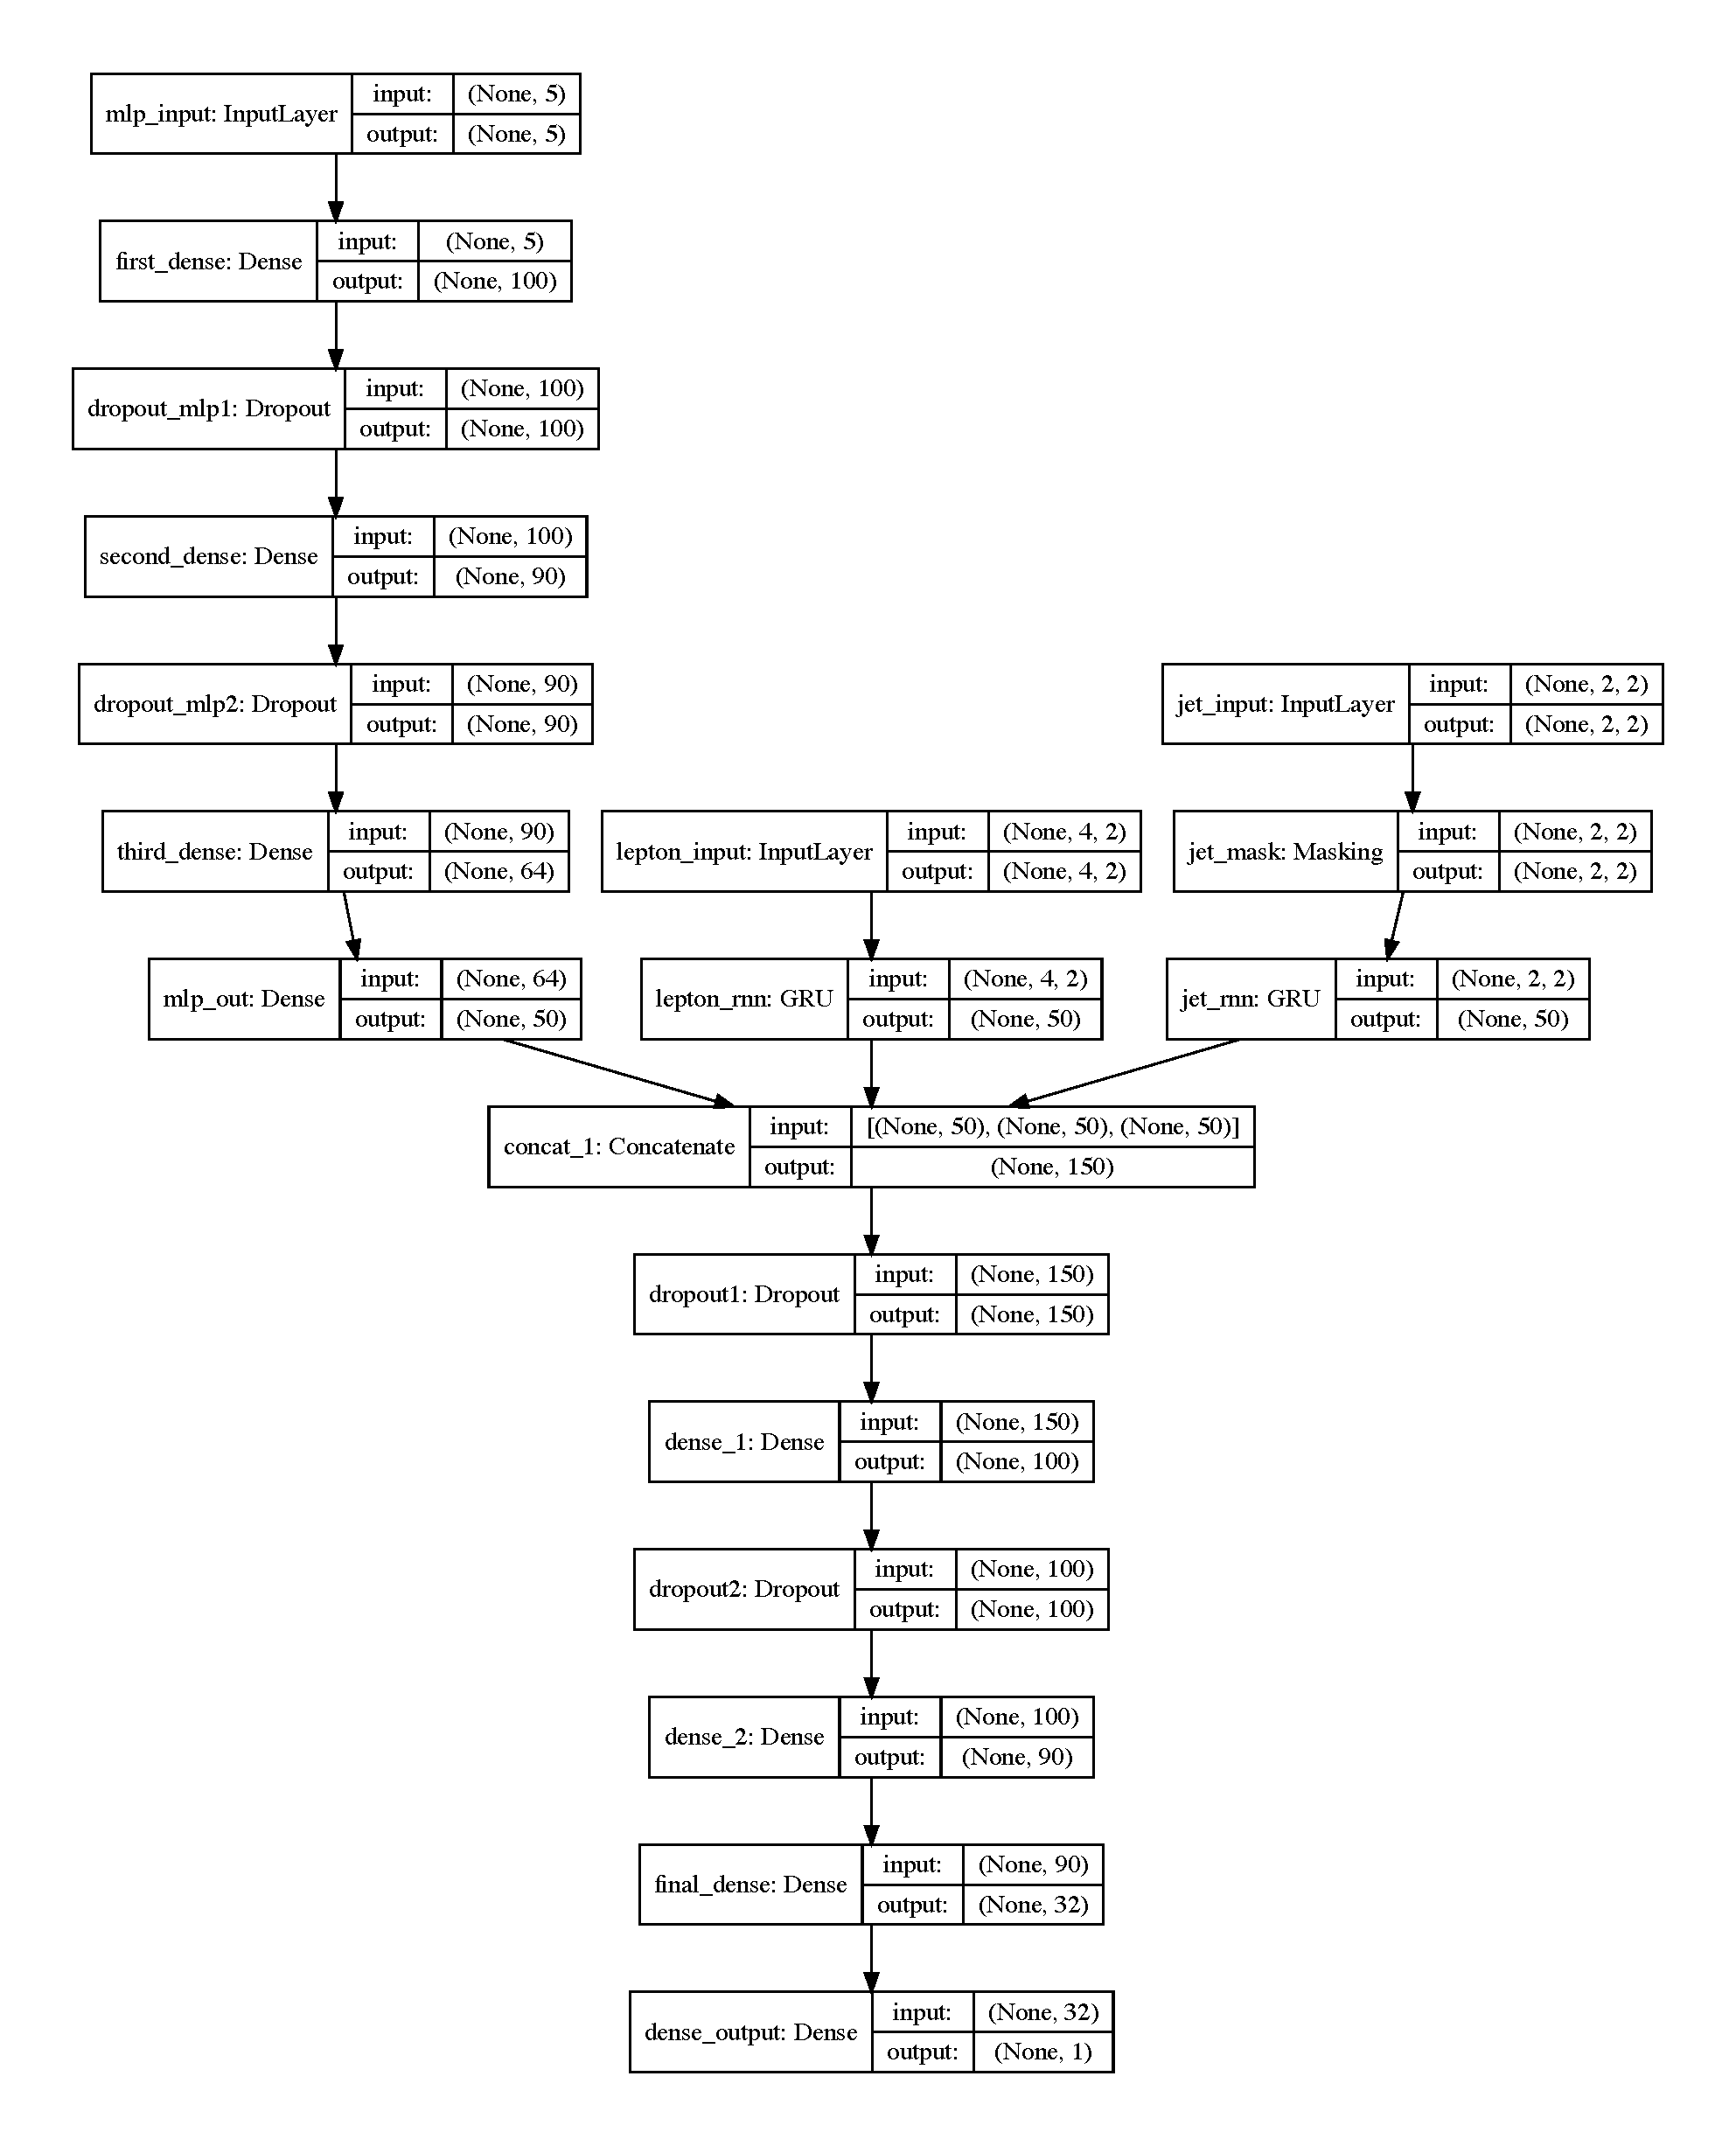
\includegraphics[width=0.49\textwidth]{figures/HMHZZ/selection/model_vbf_architecture.pdf}}
        \subfloat[]{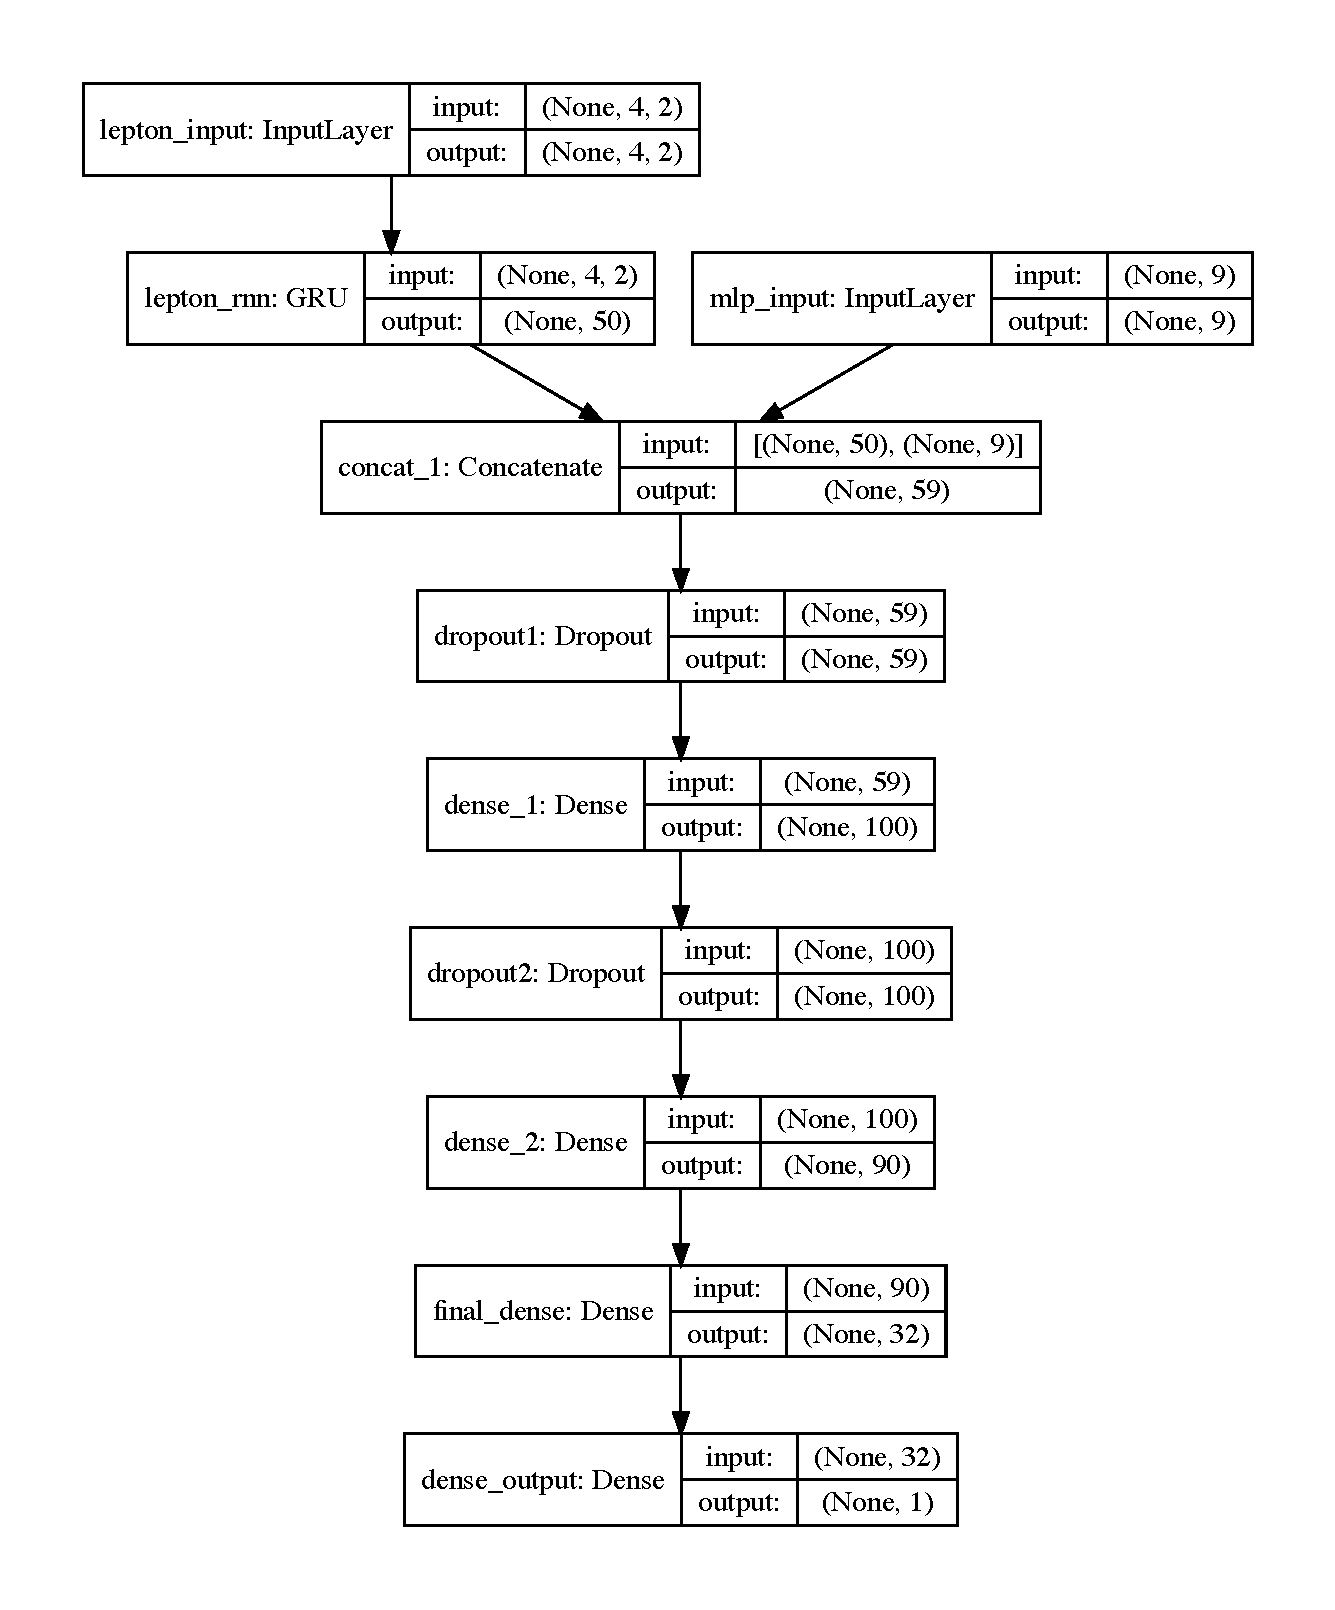
\includegraphics[width=0.49\textwidth]{figures/HMHZZ/selection/model_ggf_architecture.pdf}}
        \caption{(a) VBF DNN architecture diagram. (b) ggF DNN architecture.}
        \label{fig:dnn_arch}
\end{figure}

For training, the VBF and ggF signal samples at the masses of 200, 300, 400, 500, 600, 700, 800, 900, 1000, 1200, 1400~\gev~ are used with positive label.
The VBF (ggF) signals are only used for VBF (ggF) classifier.
The background including simulated samples of QCD and EW \qqZZ processes as well as \ggZZ process summed according to their cross section are assigned with negative labels.
In addition to the selections described in section~\ref{sec:hmhzz_eventsel}, the events used for VBF network are required to have $N_\mathrm{jets} \geq 2$, while $N_\mathrm{jets} < 2$ is required for events in ggF network,
so the training events for two network are independent.

In order to assign equivalent importance to signals with different mass assumptions, during the training, signal events are reweighted to follow the \mfl distribution from background (idea from Ref.~\cite{Baldi:2016fzo} with a modified reweighting procedure), 
as shown in figure~\ref{fig:dnn_rwt_vbf} (figure~\ref{fig:dnn_rwt_ggf}) before and after reweighting for VBF (ggF) samples.

\begin{figure}[htbp]
        \centering
        \subfloat[]{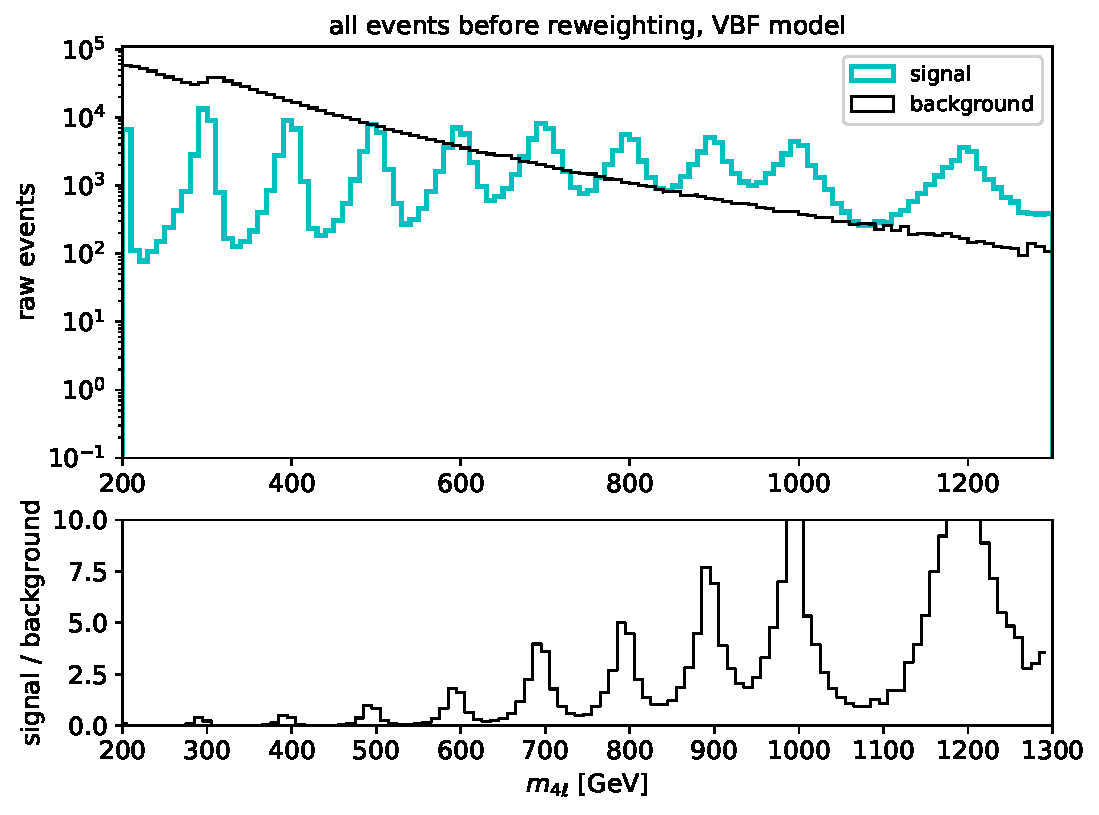
\includegraphics[width=0.48\textwidth]{{figures/HMHZZ/selection/vbf_input/m4l_before_reweighting.pdf}}}
        \subfloat[]{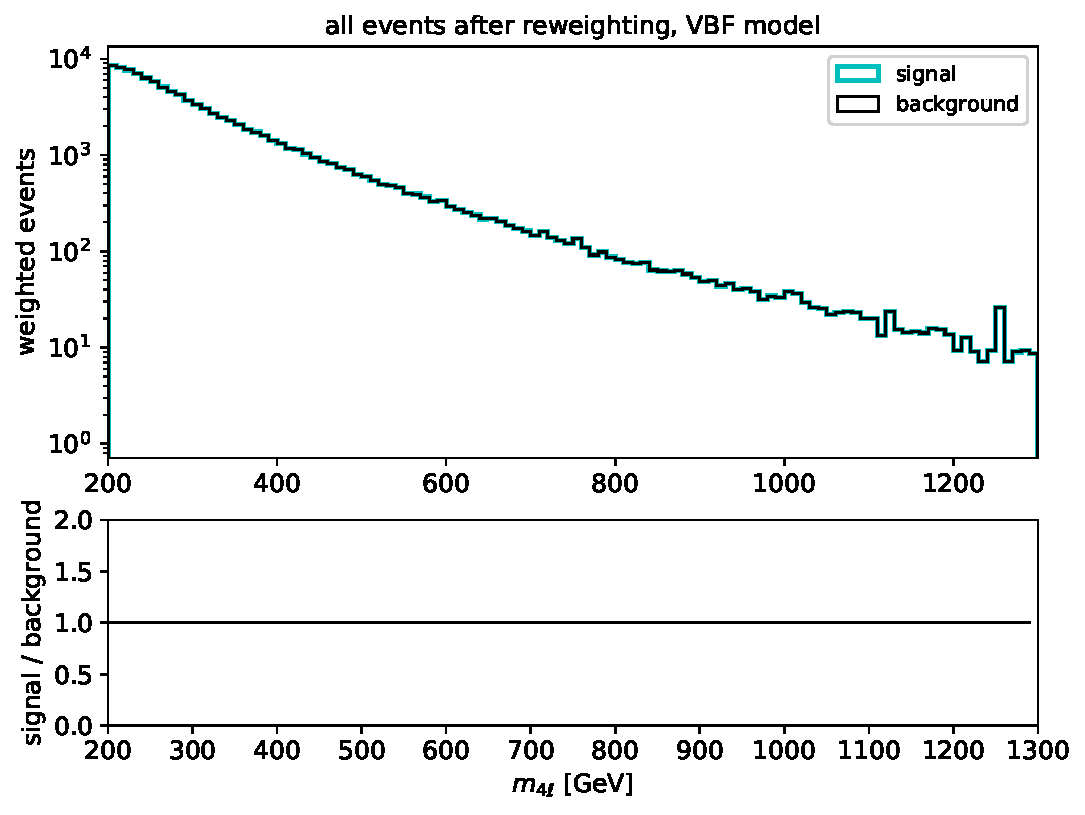
\includegraphics[width=0.48\textwidth]{{figures/HMHZZ/selection/vbf_input/m4l_after_reweighting.pdf}}}
        \caption{(a) \mfl distribution of raw (unweighted) training events for VBF signal (blue) and background (black); (b) \mfl distribution of weighted VBF signal (blue) and background (black) used at training time.}
        \label{fig:dnn_rwt_vbf}
\end{figure}

\begin{figure}[htbp]
        \centering
        \subfloat[]{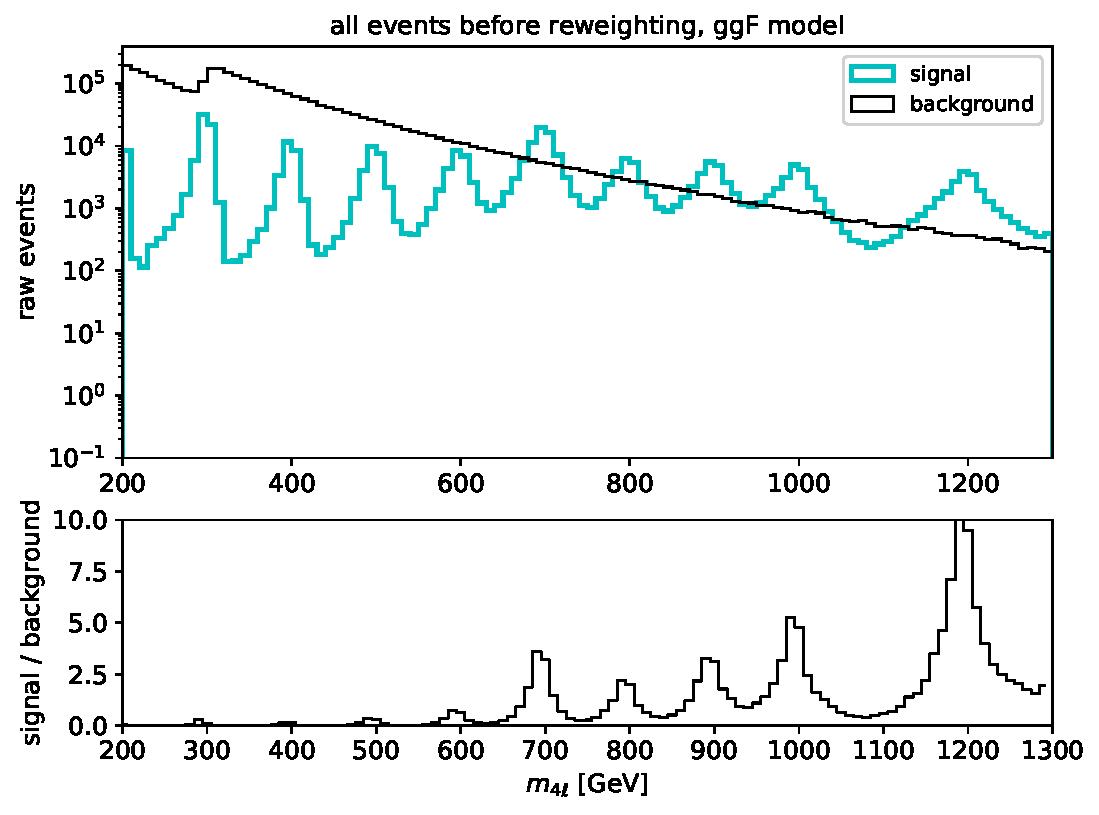
\includegraphics[width=0.48\textwidth]{{figures/HMHZZ/selection/ggf_input/m4l_all_before_reweighting.pdf}}}
        \subfloat[]{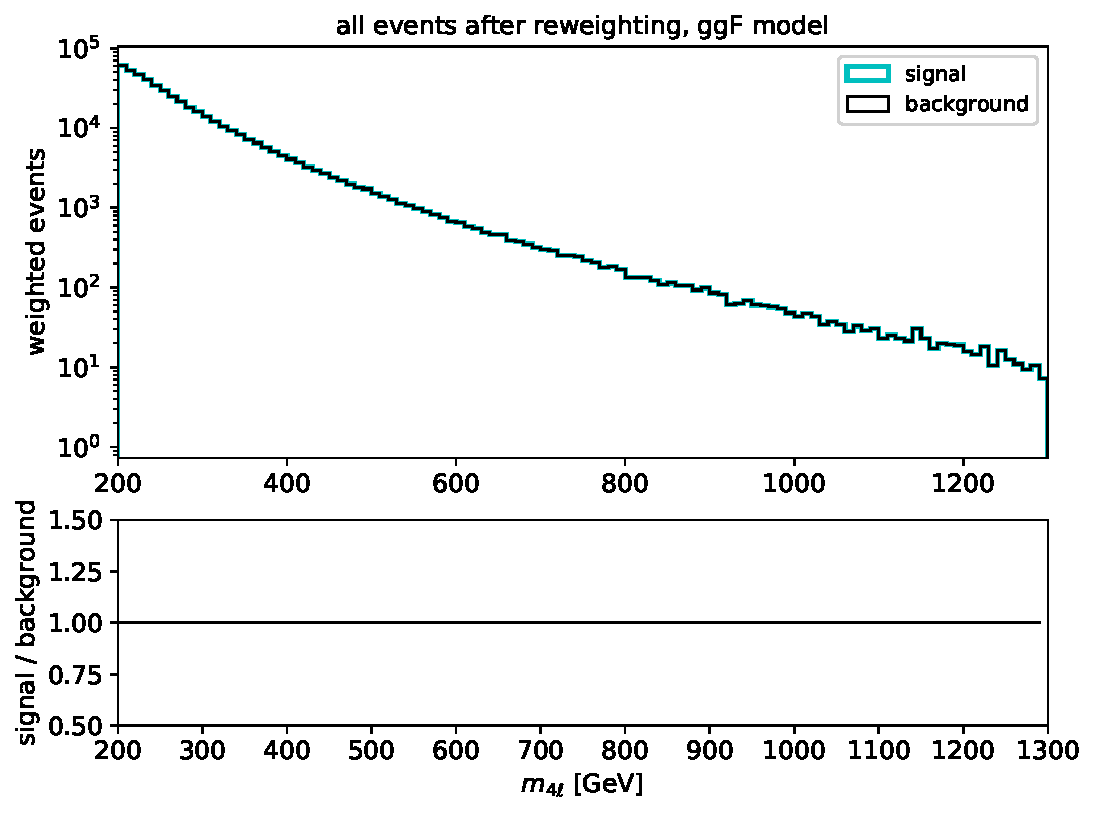
\includegraphics[width=0.48\textwidth]{{figures/HMHZZ/selection/ggf_input/m4l_all_after_reweighting.pdf}}}
        \caption{(a) \mfl distribution of raw (unweighted) training events for ggF signal (blue) and background (black); (b) \mfl distribution of weighted ggF signal (blue) and background (black) used at training time.}
        \label{fig:dnn_rwt_ggf}
\end{figure}

%After all these preparation, then the training is performed over 20 epochs with batch size of 512 (256) for VBF (ggF) network.


\textbf{Input features}

Table~\ref{tab:dnn_features_VBF} (table~\ref{tab:dnn_features_ggF}) lists the input features used for VBF (ggF) network during the training.
For VBF network, one RNN (the other one) takes the \pt and $\eta$ of \pt-ordered four leptons (two leading jets) as input features, which intends to study the time relationship from particle decay between leptons (jets).
For ggF network, the only one RNN model takes the \pt and $\eta$ of \pt-ordered four leptons as inputs.

\begin{table}
\caption{
Input features used in the ``VBF-classifier'' for the \llll analysis.
The RNN stands for the recurrent neural network and MLP for the multilayer perceptron.
\label{tab:dnn_features_VBF}}
\centering
\begingroup
\setlength{\tabcolsep}{10pt}
\renewcommand{\arraystretch}{1.0}
\begin{tabularx}{\textwidth}{ccX}
\toprule
Model &    Inputs                                & Description \\ \hline
\multirow{4}{*}{RNN}    & $\pt^{\text{j0}, \text{j1}}$            & transverse momenta of the two leading jets \\
                        & $\eta^{\text{j0}, \text{j1}}$           & pseudorapidity of the two leading jets \\
                        & $\pt^{\ell0, \ell1, \ell2, \ell3}$      & transverse momenta of the four leptons \\
                        & $\eta^{\ell0, \ell1, \ell2, \ell3}$     & pseudorapidity of the four leptons \\
                        \midrule
\multirow{5}{*}{MLP}    & \mfl                          & invariant mass of the four lepton system \\
                        & \mjj                          & invariant mass of the two leading jet system \\
                        & $\pt^{\text{jj}}$             & transverse momentum of the two leading jet system \\
                        & $\Delta\eta_{\text{H,j}}$     & difference in pseudorapidity between the four lepton system and the leading jet \\
                        & min$\Delta R_{\text{jZ}}$     & minimum distance between one of the two lepton pairs and a jet \\

\bottomrule
\end{tabularx}
\endgroup
\end{table}

\begin{table}
    \caption{
    Input features used in the ``ggF-classifier'' for the \llll analysis.
    The RNN stands for the recurrent neural network and MLP for the multilayer perceptron.
    \label{tab:dnn_features_ggF}}
    \centering
\begingroup
\setlength{\tabcolsep}{10pt}
\renewcommand{\arraystretch}{1.0}
\begin{tabularx}{\textwidth}{ccX}
\toprule
Model & Inputs                                & Description \\ \hline
\multirow{2}{*}{RNN}    & $\pt^{\ell0, \ell1, \ell2, \ell3}$      & transverse momenta of the four leptons \\
                        & $\eta^{\ell0, \ell1, \ell2, \ell3}$     & pseudorapidity of the four leptons \\
\midrule
\multirow{9}{*}{MLP}    & \mfl                & invariant mass of the four lepton system \\
                        & $\pt^{4\ell}$       & transverse momentum of the four lepton system \\
                        & $\eta^{4\ell}$      & pseudorapidity of the four lepton system \\
                        & $\cos\theta^*$      & production angle of the leading $Z$ defined in the four lepton rest frame \\
                        & $\cos\theta_{1}$    & angle between the negative final state lepton and the direction of flight of leading $Z$ in the $Z$ rest frame \\
                        & $\cos\theta_{2}$    & angle between the negative final state lepton and the direction of flight of sub-leading $Z$ in the $Z$ rest frame \\
                        & $\Phi$              & angle between the decay planes of the four final state leptons expressed in the four lepton rest frame \\
                        & $\pt^{\text{j0}}$   & transverse momentum of the leading jet \\
                        & $\eta^{\text{j0}}$  & pseudorapidity of the leading jet \\

\bottomrule
    \end{tabularx}
    \endgroup
    \end{table}


%Figure~\ref{fig:dnn_vbf_distribution} (figure~\ref{fig:dnn_ggf_distribution}) shows the distributions of input features with events before training reweighting for VBF (ggF) network of background and 4 signal samples at mass points of 300, 700, 1400 and 2000~\gev.
%
%\begin{figure}[htbp]
%        \captionsetup[subfigure]{labelformat=empty}
%        \centering
%        \subfloat[]{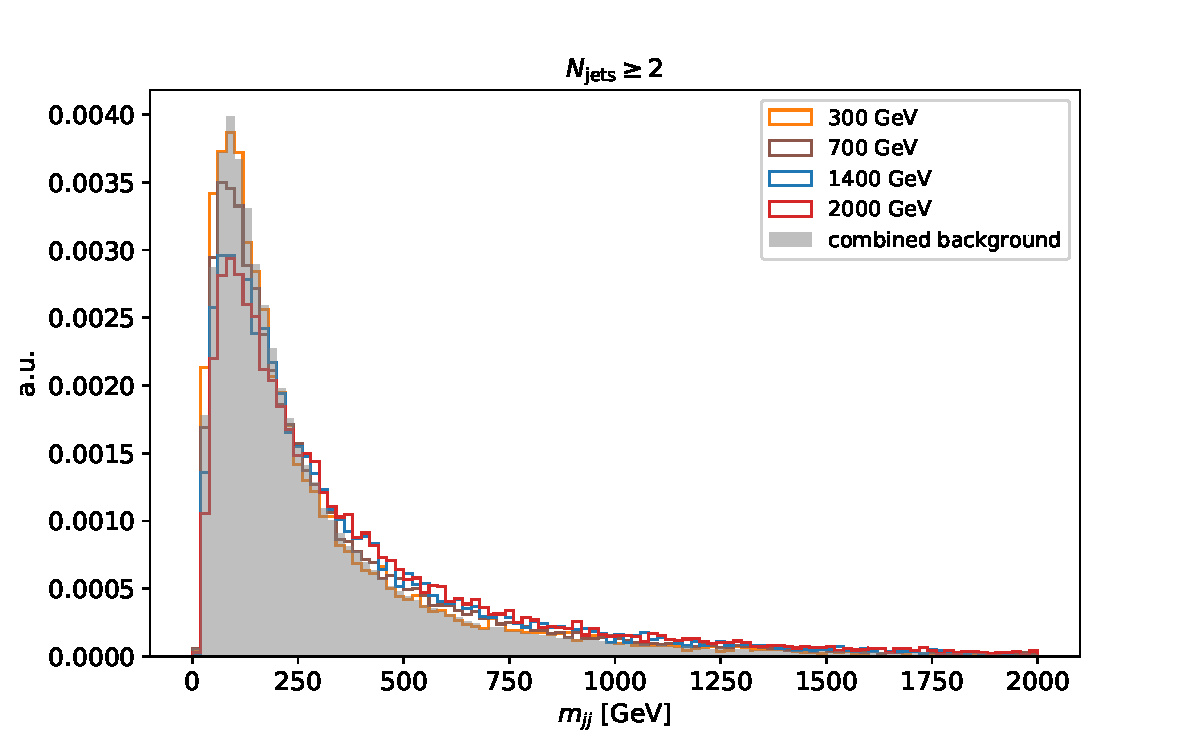
\includegraphics[width=0.19\textwidth]{figures/HMHZZ/selection/vbf_input/input_comparison_300_to_2000_0_score_dijet_invmass}}
%        \subfloat[]{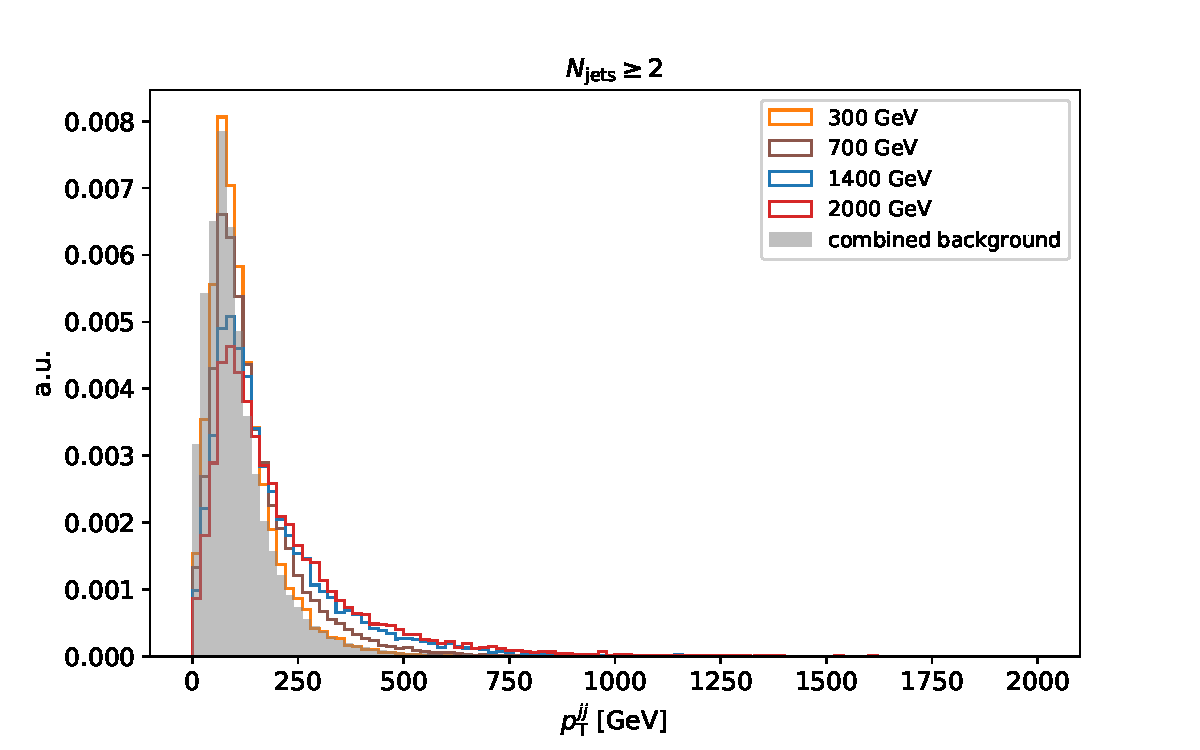
\includegraphics[width=0.19\textwidth]{figures/HMHZZ/selection/vbf_input/input_comparison_300_to_2000_2_score_dijet_pt}}
%        \subfloat[]{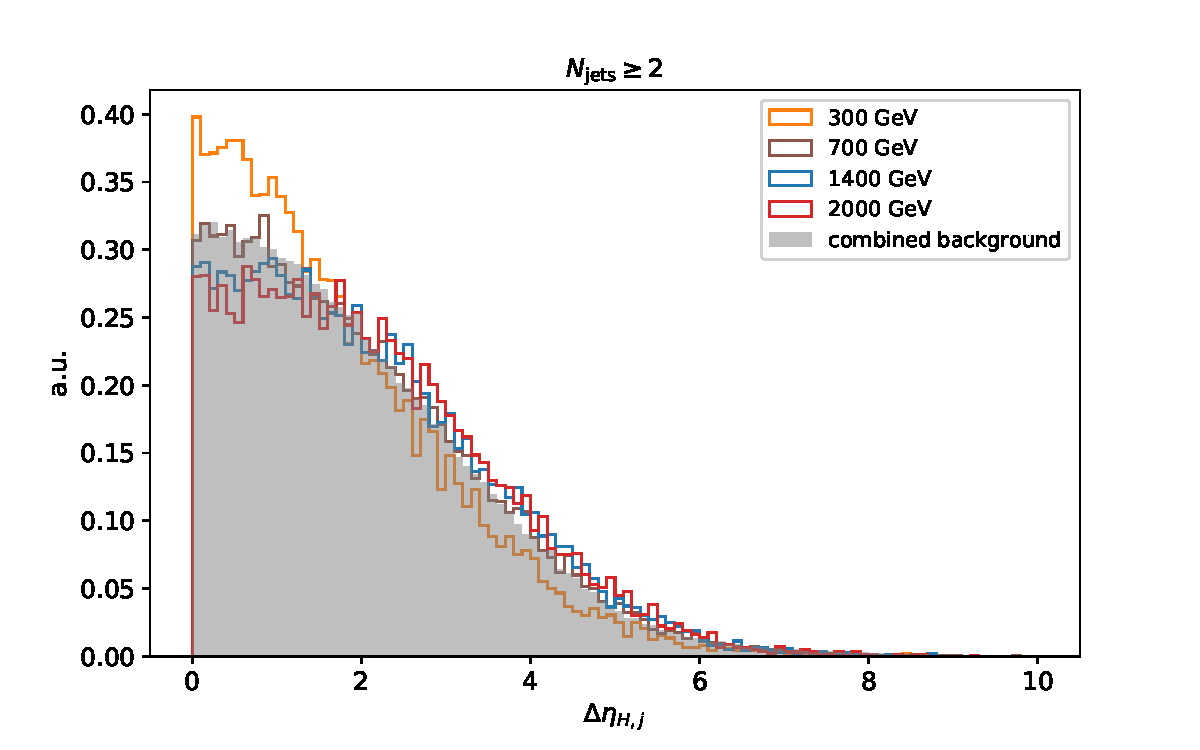
\includegraphics[width=0.19\textwidth]{figures/HMHZZ/selection/vbf_input/input_comparison_300_to_2000_3_score_eta_zepp_ZZ}}
%        \subfloat[]{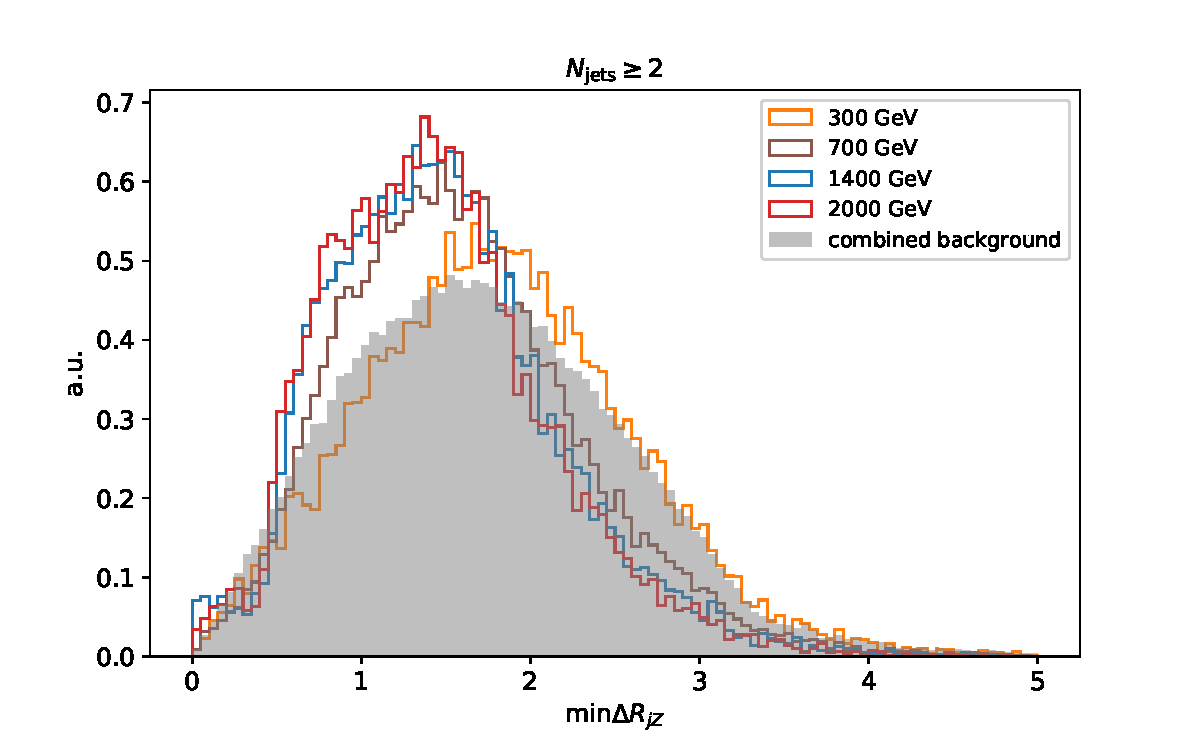
\includegraphics[width=0.19\textwidth]{figures/HMHZZ/selection/vbf_input/input_comparison_300_to_2000_4_score_min_dR_jZ}}
%        \subfloat[]{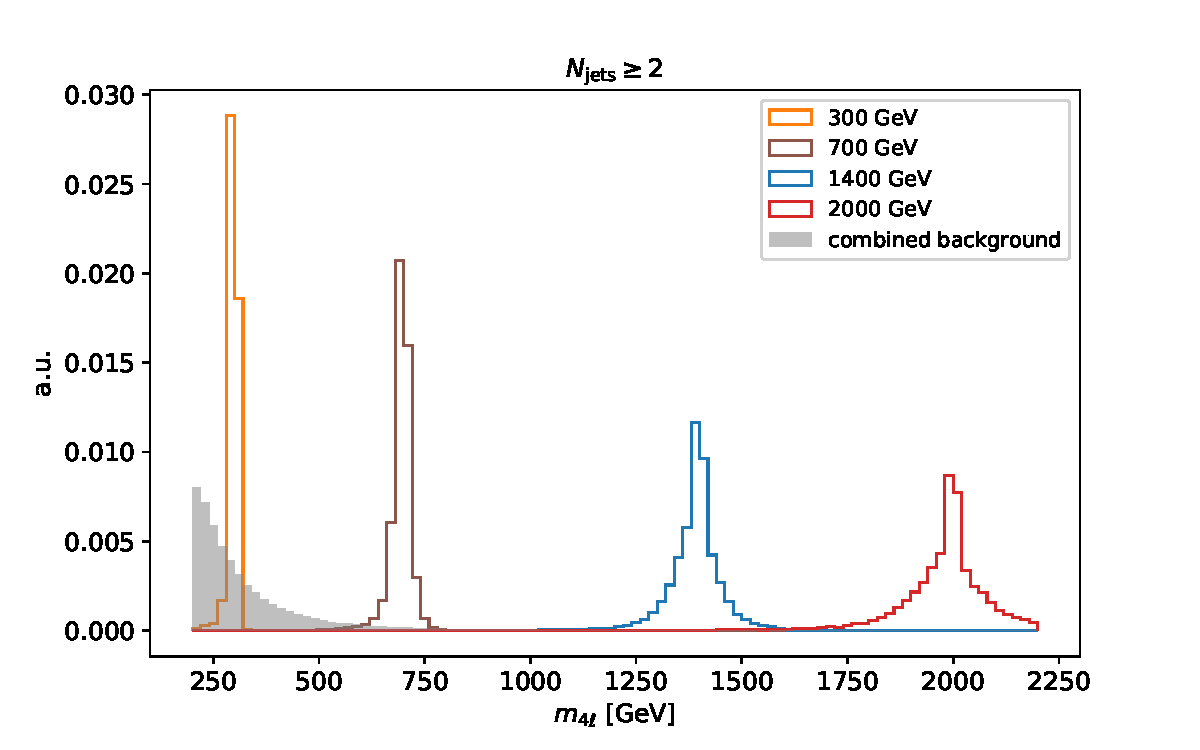
\includegraphics[width=0.19\textwidth]{figures/HMHZZ/selection/vbf_input/input_comparison_300_to_2000_5_score_m4l_unconstrained}}\\
%
%        \subfloat[]{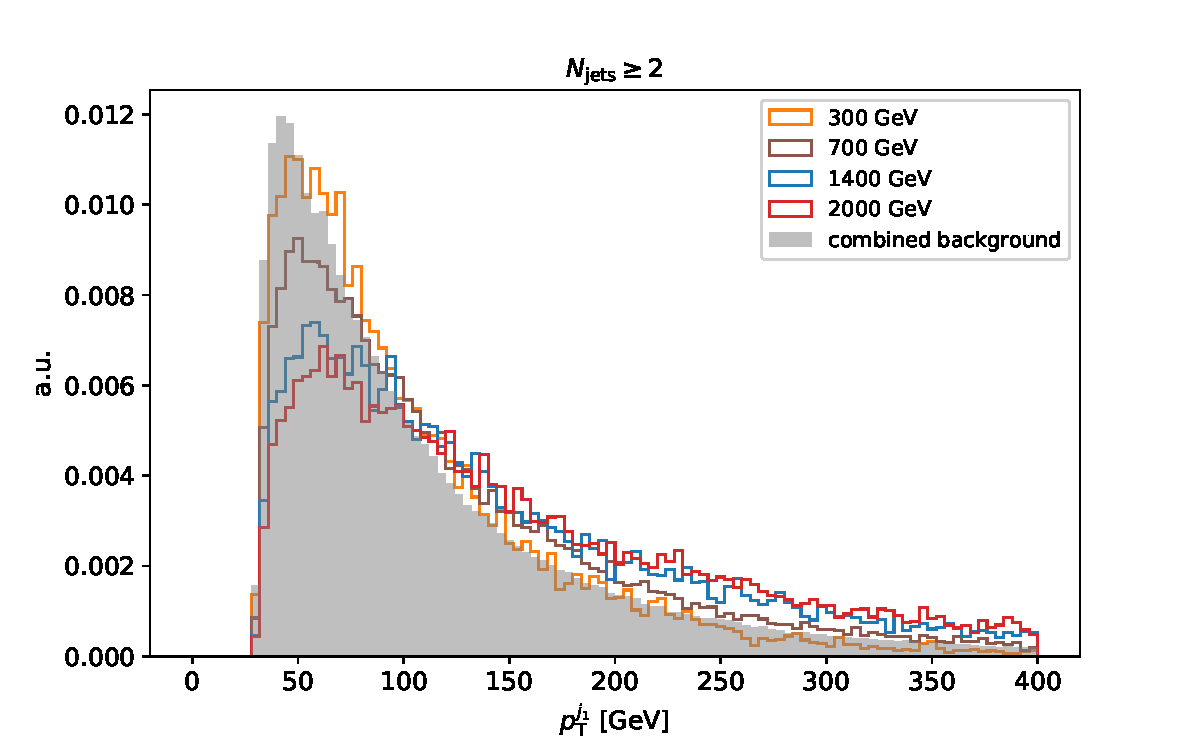
\includegraphics[width=0.24\textwidth]{figures/HMHZZ/selection/vbf_input/input_comparison_300_to_2000_23_score_j_1_pt}}
%        \subfloat[]{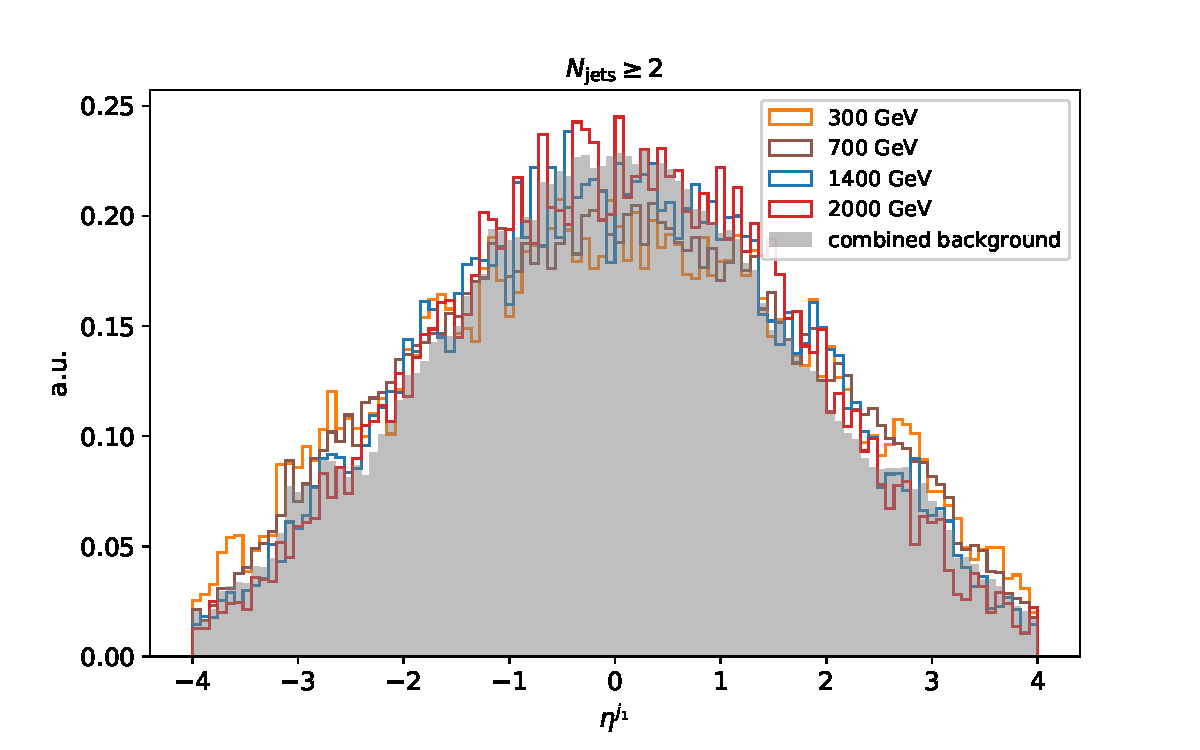
\includegraphics[width=0.24\textwidth]{figures/HMHZZ/selection/vbf_input/input_comparison_300_to_2000_24_score_j_1_eta}}
%        \subfloat[]{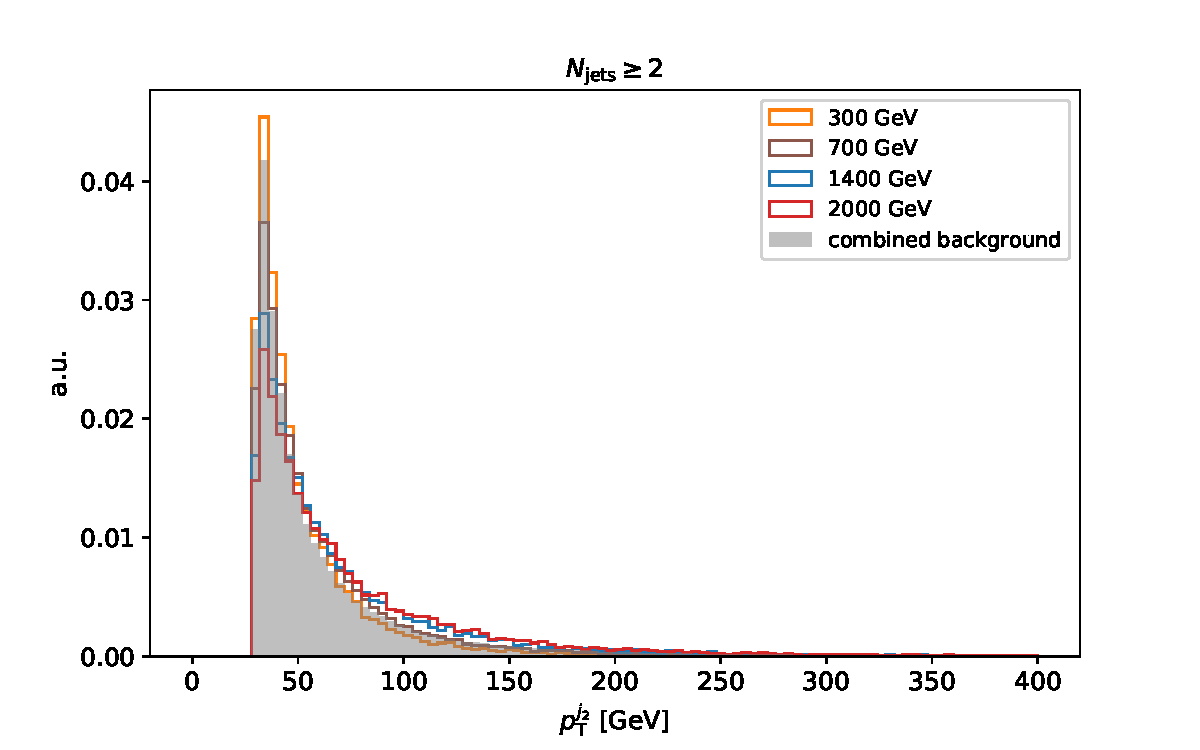
\includegraphics[width=0.24\textwidth]{figures/HMHZZ/selection/vbf_input/input_comparison_300_to_2000_25_score_j_2_pt}}
%        \subfloat[]{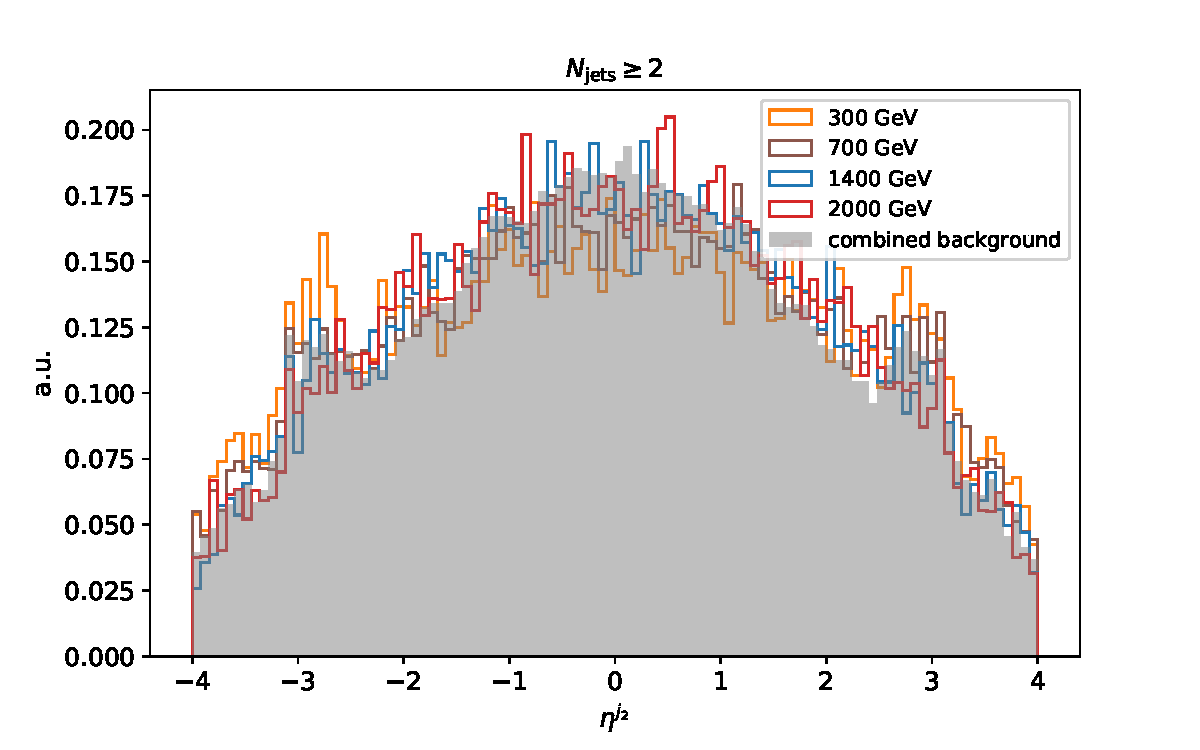
\includegraphics[width=0.24\textwidth]{figures/HMHZZ/selection/vbf_input/input_comparison_300_to_2000_26_score_j_2_eta}}\\
%
%        \subfloat[]{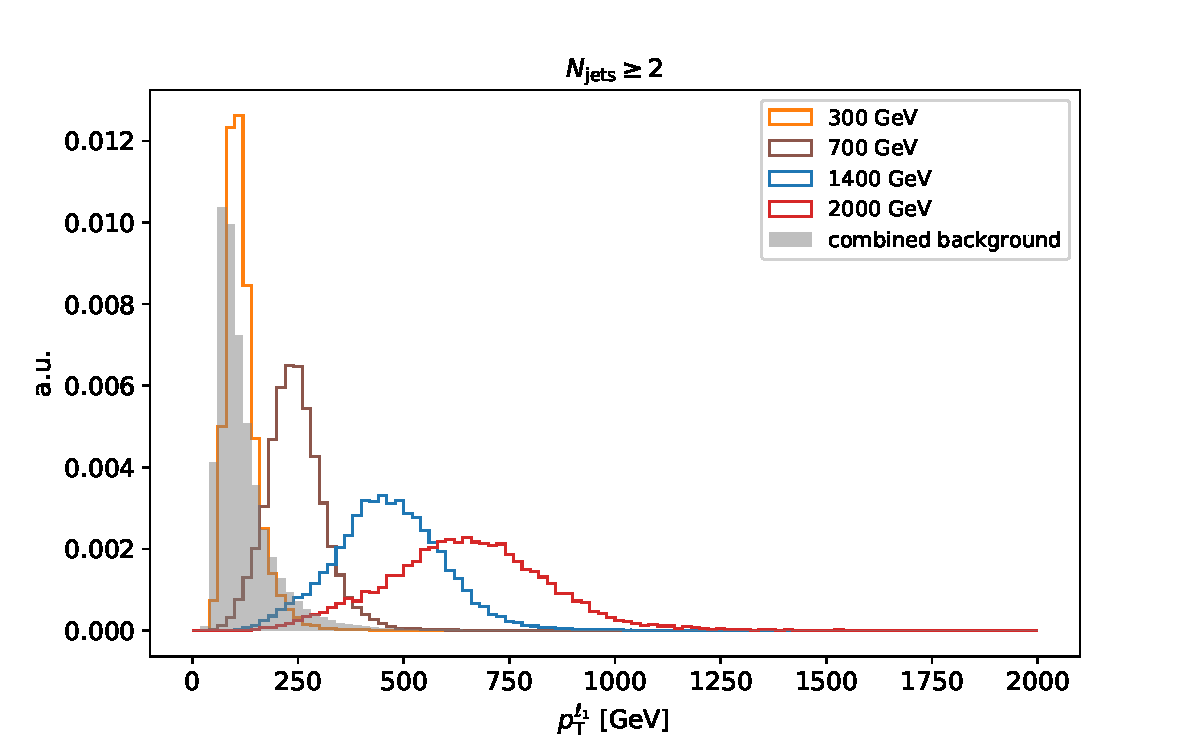
\includegraphics[width=0.24\textwidth]{figures/HMHZZ/selection/vbf_input/input_comparison_300_to_2000_15_score_lep_1_pt}}
%        \subfloat[]{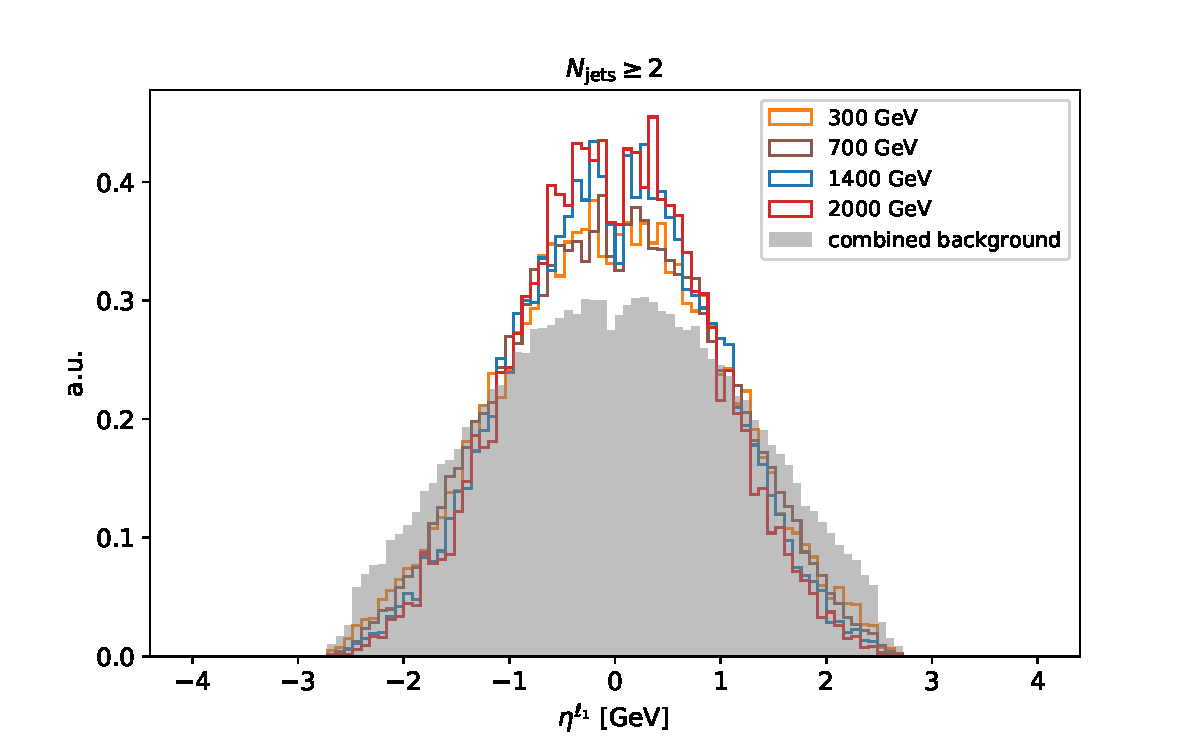
\includegraphics[width=0.24\textwidth]{figures/HMHZZ/selection/vbf_input/input_comparison_300_to_2000_16_score_lep_1_eta}}
%        \subfloat[]{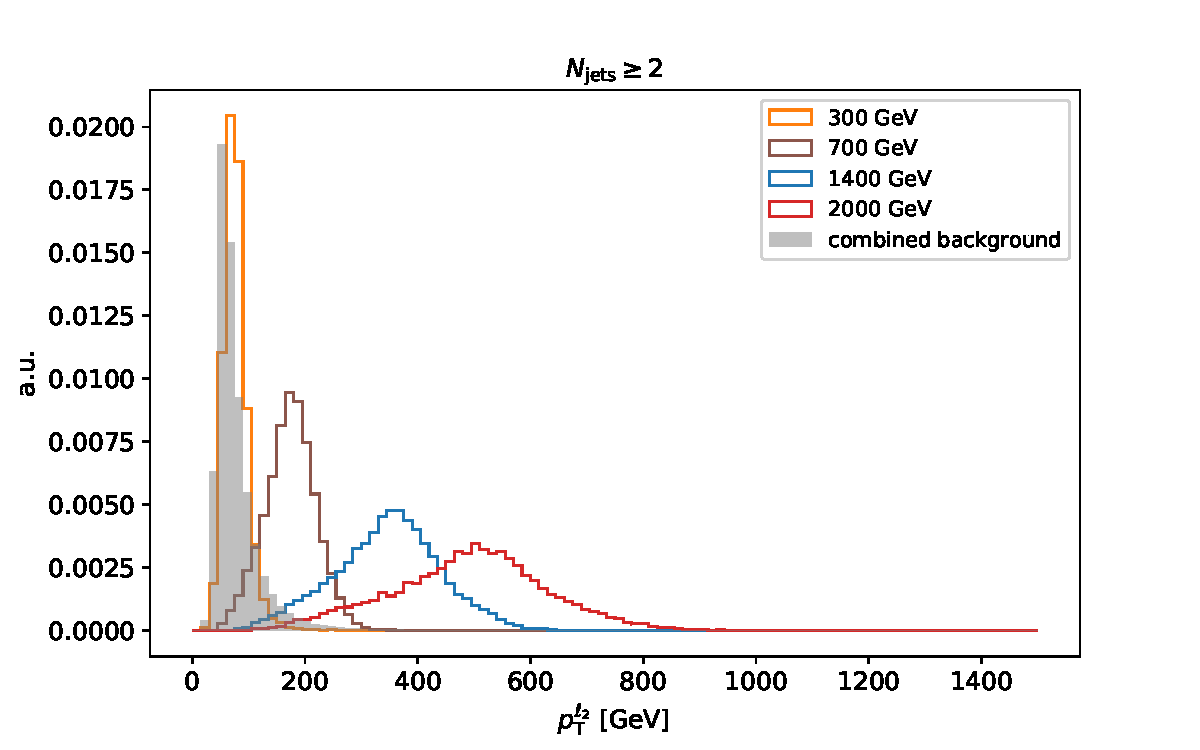
\includegraphics[width=0.24\textwidth]{figures/HMHZZ/selection/vbf_input/input_comparison_300_to_2000_17_score_lep_2_pt}}
%        \subfloat[]{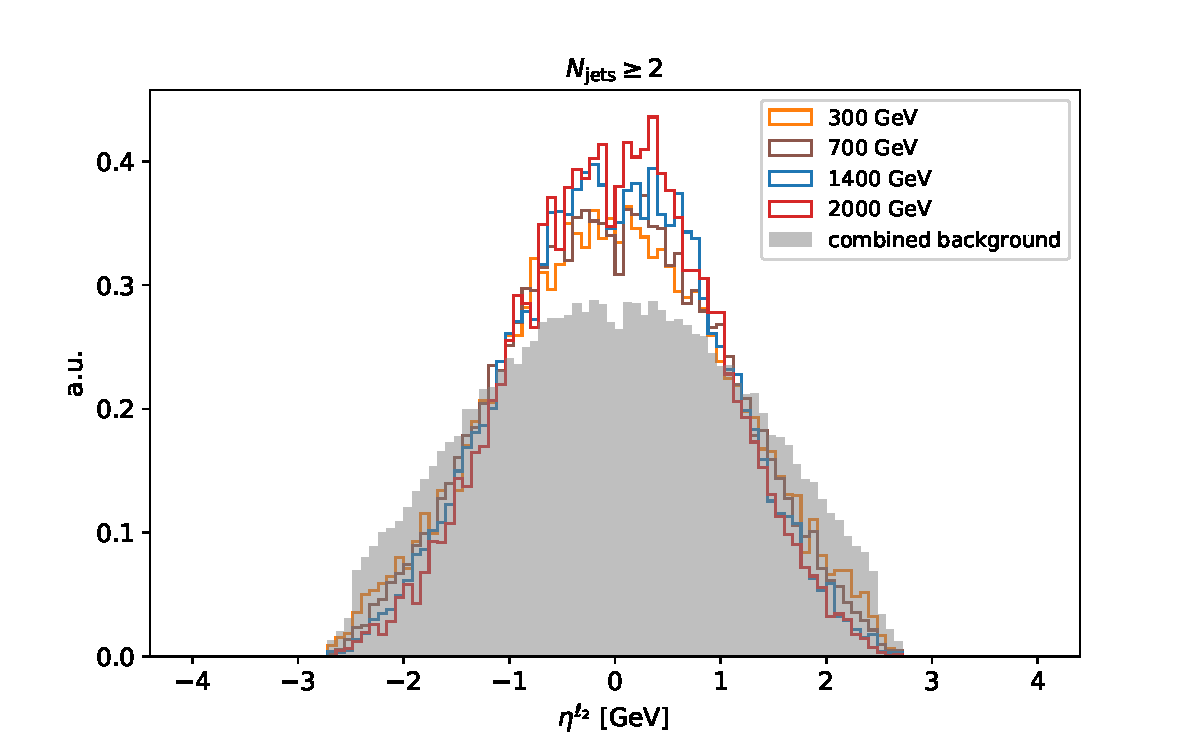
\includegraphics[width=0.24\textwidth]{figures/HMHZZ/selection/vbf_input/input_comparison_300_to_2000_18_score_lep_2_eta}}\\
%
%        \subfloat[]{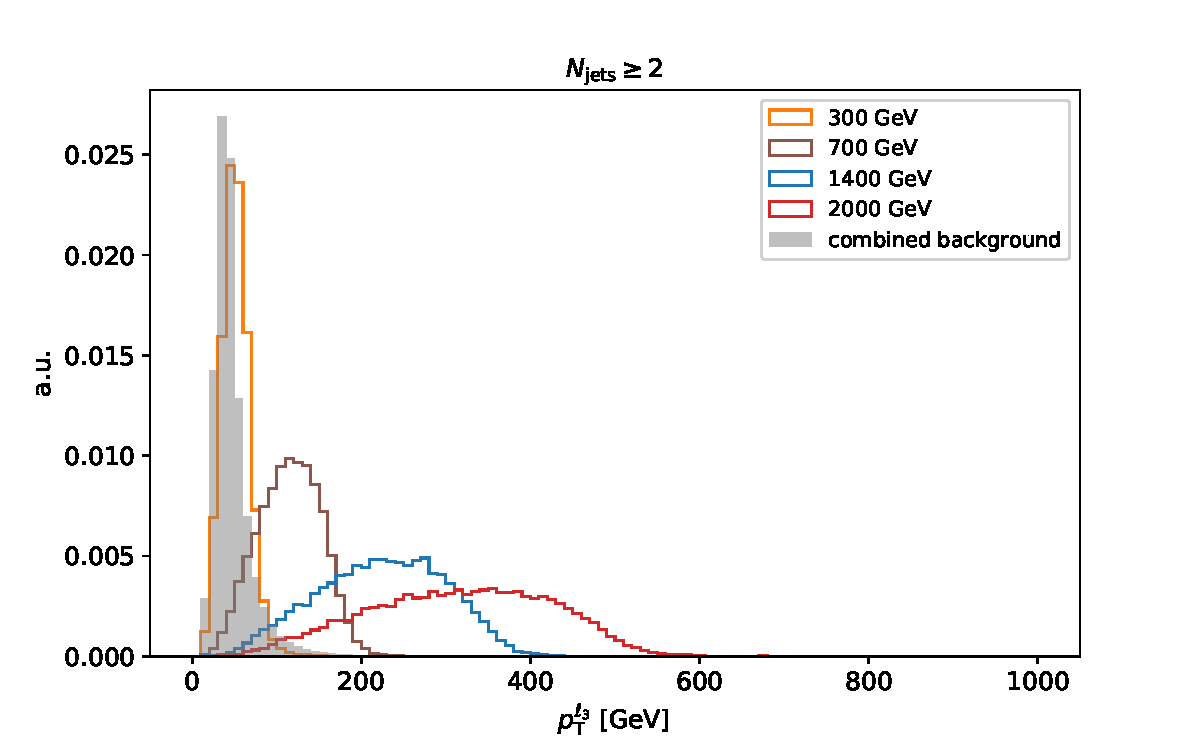
\includegraphics[width=0.24\textwidth]{figures/HMHZZ/selection/vbf_input/input_comparison_300_to_2000_19_score_lep_3_pt}}
%        \subfloat[]{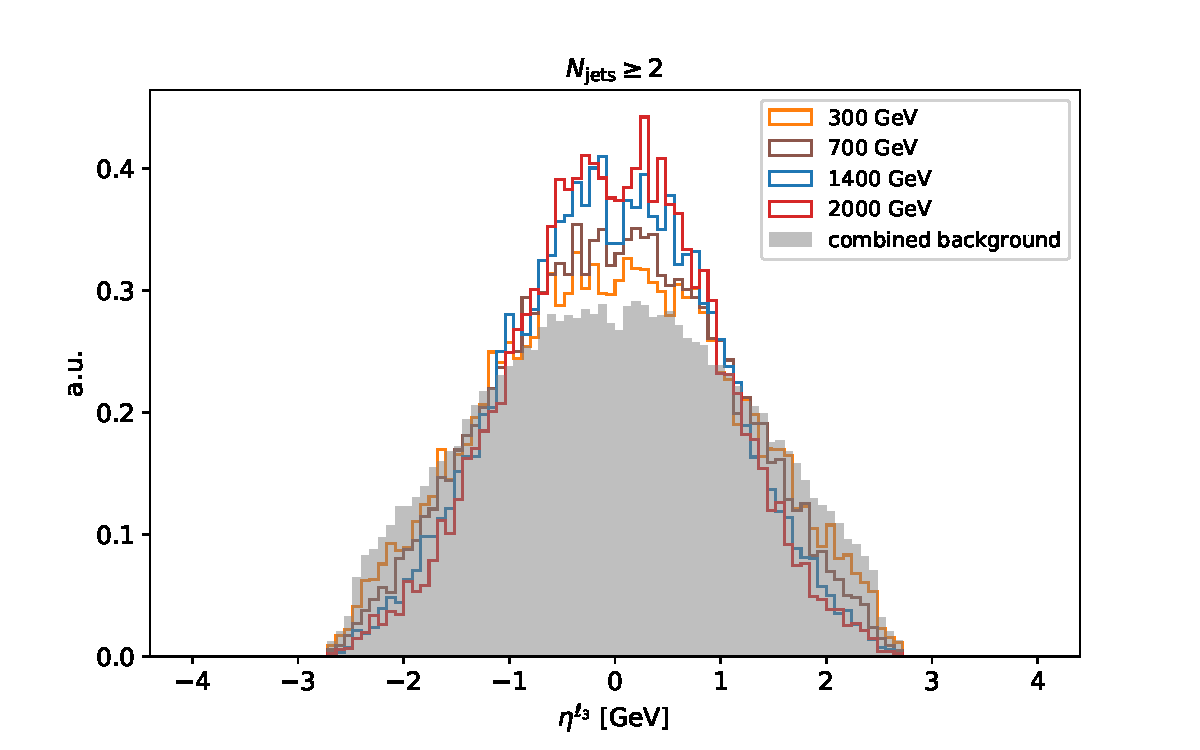
\includegraphics[width=0.24\textwidth]{figures/HMHZZ/selection/vbf_input/input_comparison_300_to_2000_20_score_lep_3_eta}}
%        \subfloat[]{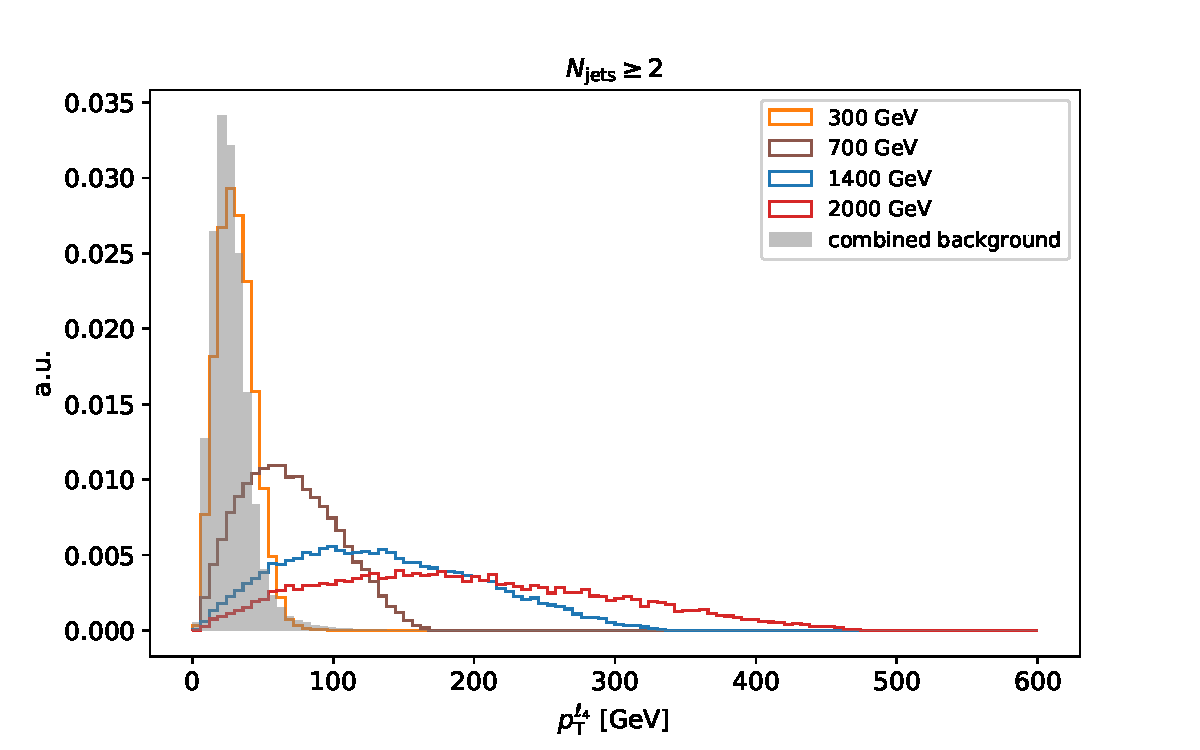
\includegraphics[width=0.24\textwidth]{figures/HMHZZ/selection/vbf_input/input_comparison_300_to_2000_21_score_lep_4_pt}}
%        \subfloat[]{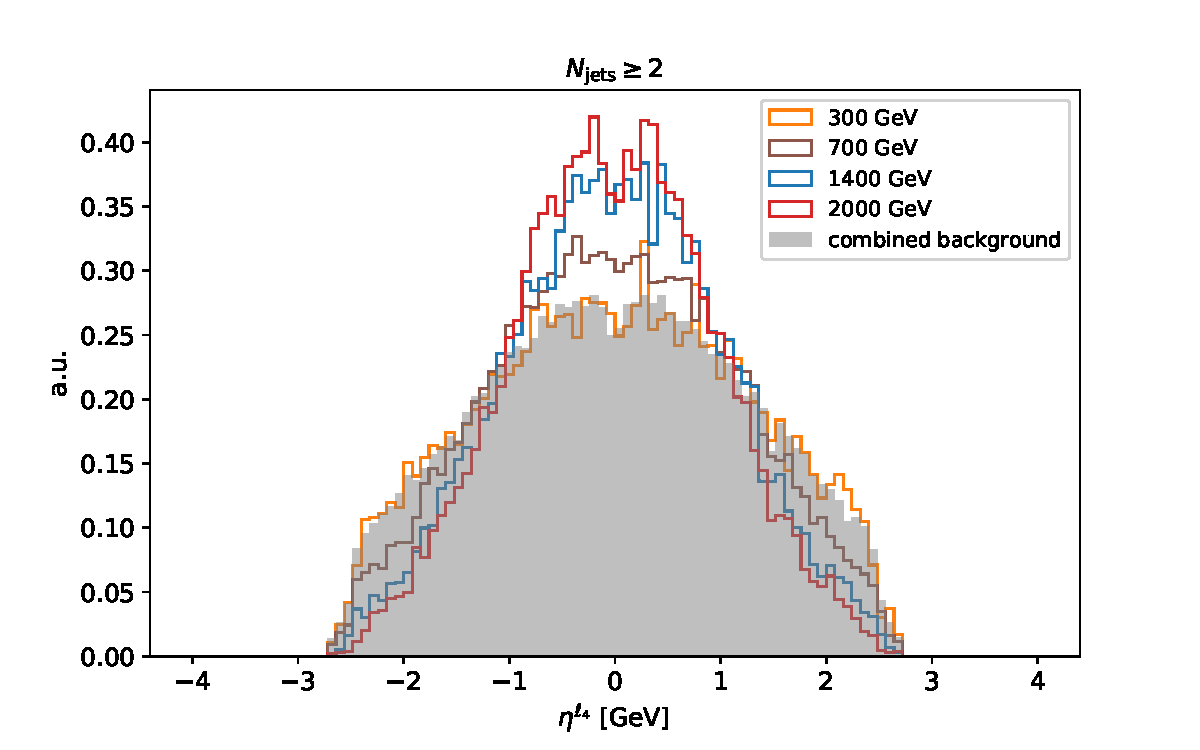
\includegraphics[width=0.24\textwidth]{figures/HMHZZ/selection/vbf_input/input_comparison_300_to_2000_22_score_lep_4_eta}}\\
%        \caption{Distributions of input features as listed in table~\ref{tab:dnn_features_vbf} for the VBF network of signals at mass points of 300, 700, 1400, 2000~\gev (coloured) and the background (grey). Only events satisfying the training selection of $N_\mathrm{jets}\geq2$ are shown.}
%        \label{fig:dnn_vbf_distribution}
%\end{figure}

%\begin{figure}[htbp]
%        \centering
%        \captionsetup[subfigure]{labelformat=empty}
%        \subfloat[]{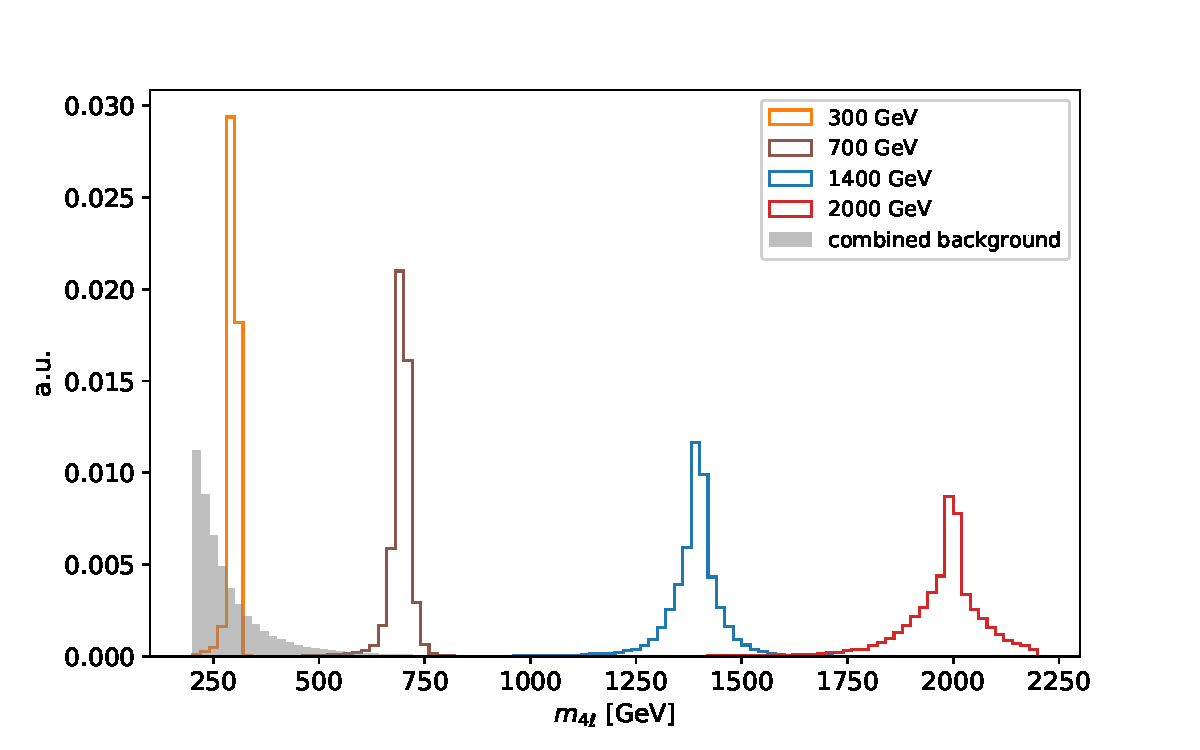
\includegraphics[width=0.24\textwidth]{figures/HMHZZ/selection/ggf_input/input_comparison_300_to_2000_5_score_m4l_unconstrained}}
%        \subfloat[]{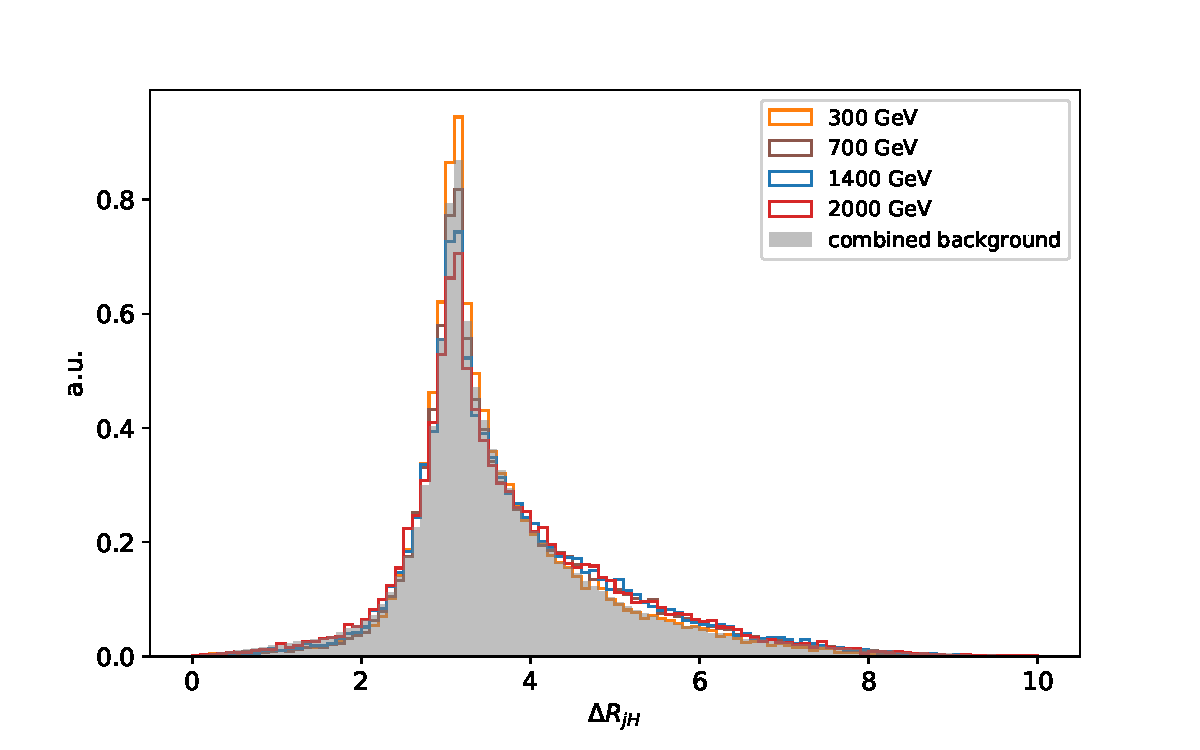
\includegraphics[width=0.24\textwidth]{figures/HMHZZ/selection/ggf_input/input_comparison_300_to_2000_6_score_dR_jH}}
%        \subfloat[]{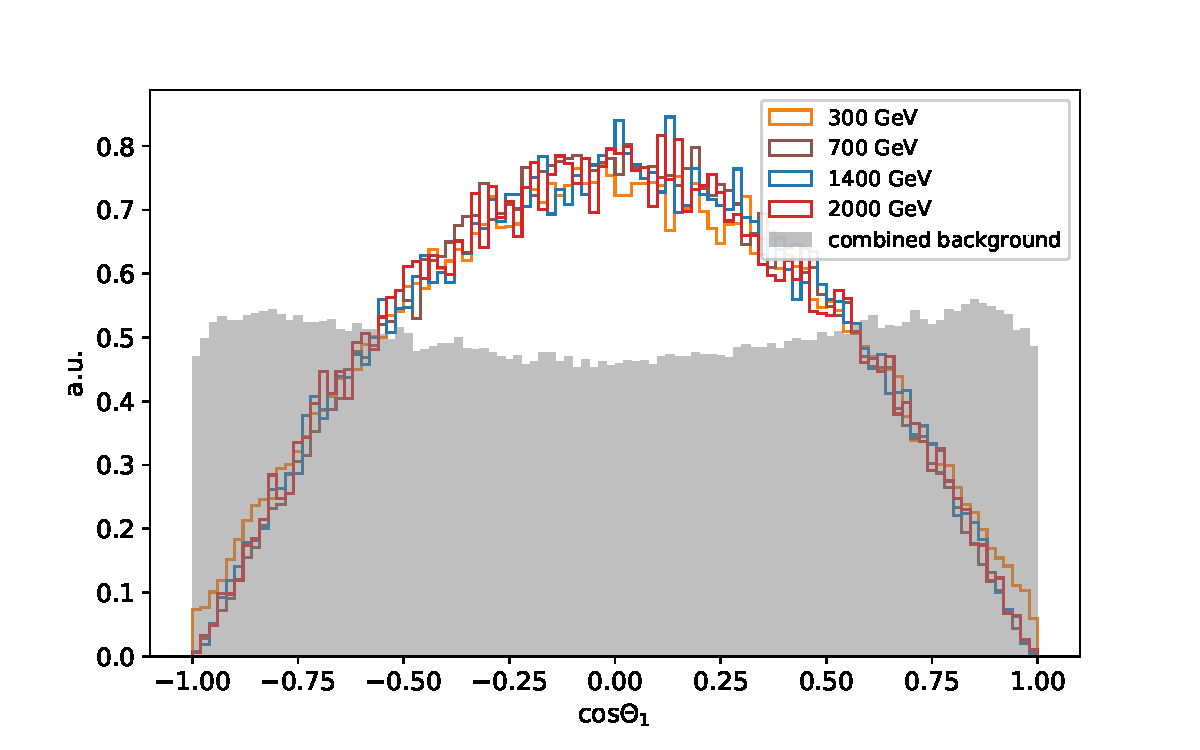
\includegraphics[width=0.24\textwidth]{figures/HMHZZ/selection/ggf_input/input_comparison_300_to_2000_7_score_cth1_unconstrained}}
%        \subfloat[]{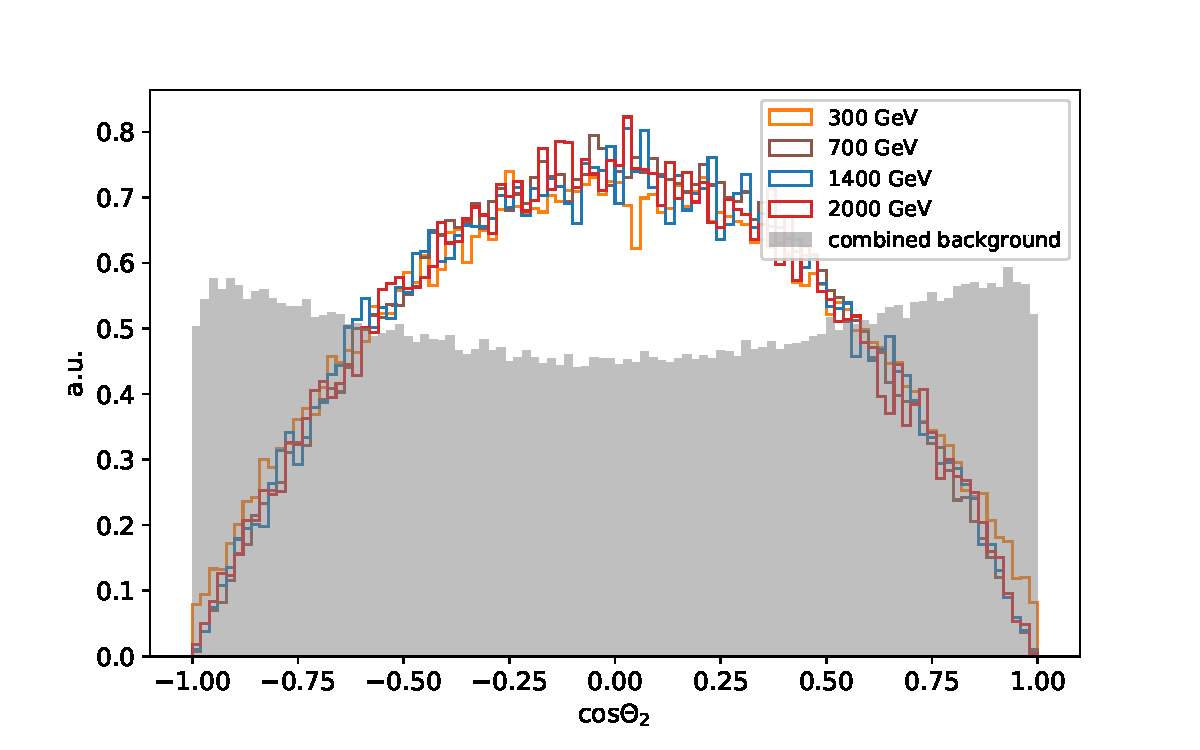
\includegraphics[width=0.24\textwidth]{figures/HMHZZ/selection/ggf_input/input_comparison_300_to_2000_8_score_cth2_unconstrained}}\\
%
%        \subfloat[]{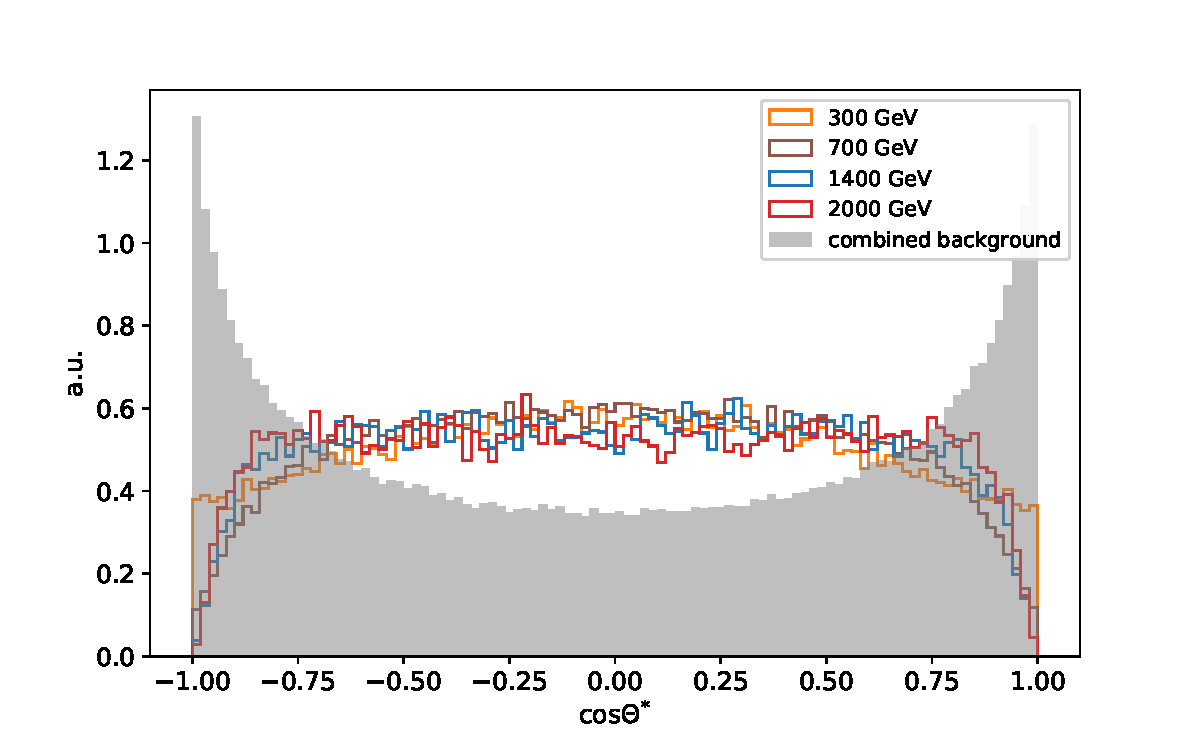
\includegraphics[width=0.24\textwidth]{figures/HMHZZ/selection/ggf_input/input_comparison_300_to_2000_9_score_cthstr_unconstrained}}
%        \subfloat[]{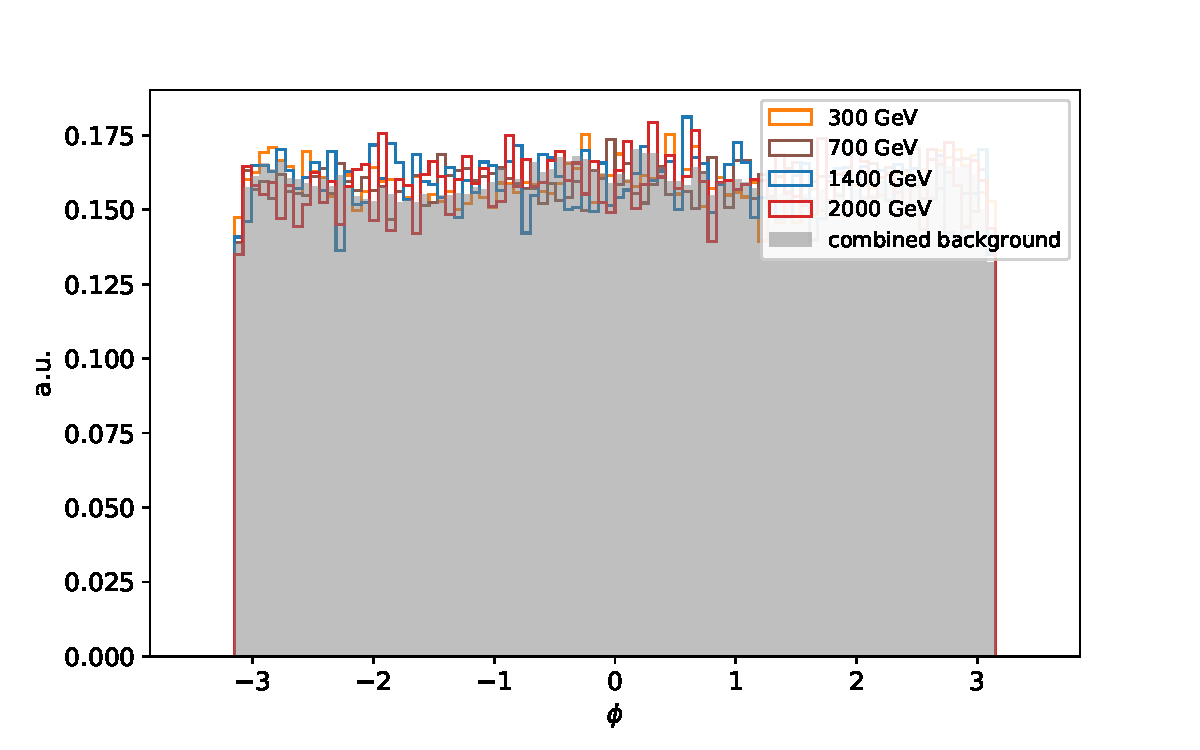
\includegraphics[width=0.24\textwidth]{figures/HMHZZ/selection/ggf_input/input_comparison_300_to_2000_10_score_phi_unconstrained}}
%        \subfloat[]{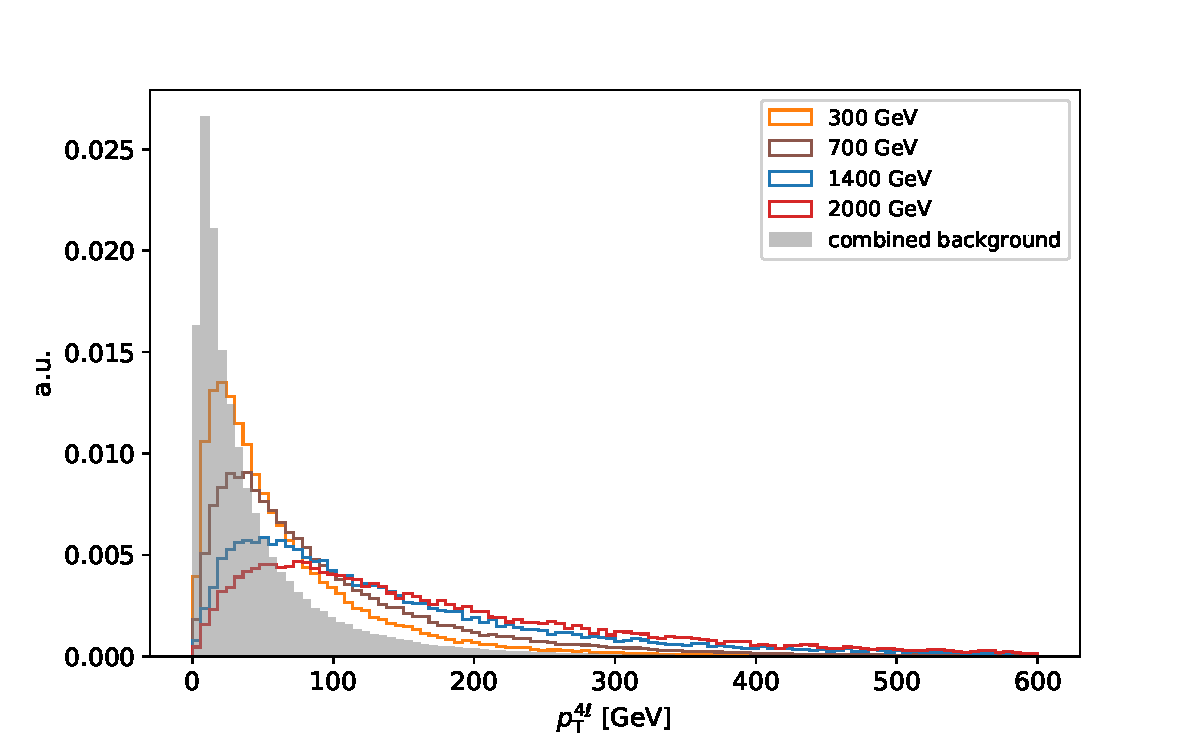
\includegraphics[width=0.24\textwidth]{figures/HMHZZ/selection/ggf_input/input_comparison_300_to_2000_11_score_pt4l_unconstrained}}
%        \subfloat[]{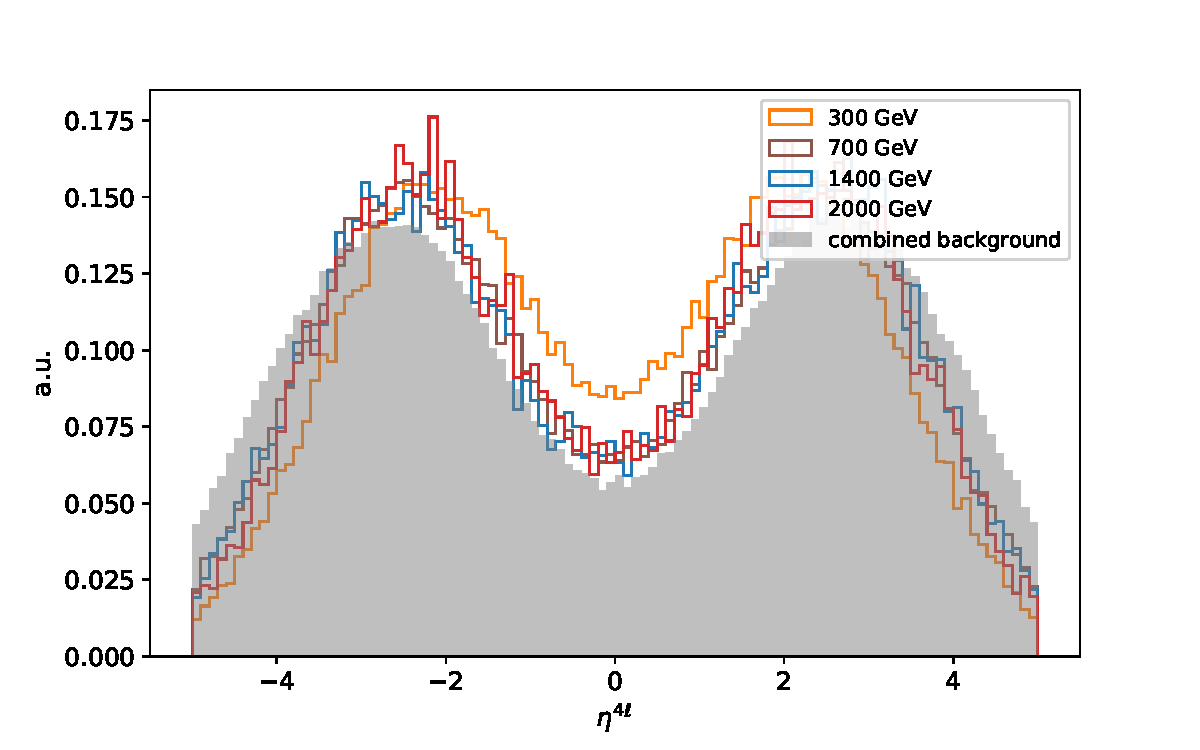
\includegraphics[width=0.24\textwidth]{figures/HMHZZ/selection/ggf_input/input_comparison_300_to_2000_12_score_eta4l_unconstrained}}\\
%
%        \subfloat[]{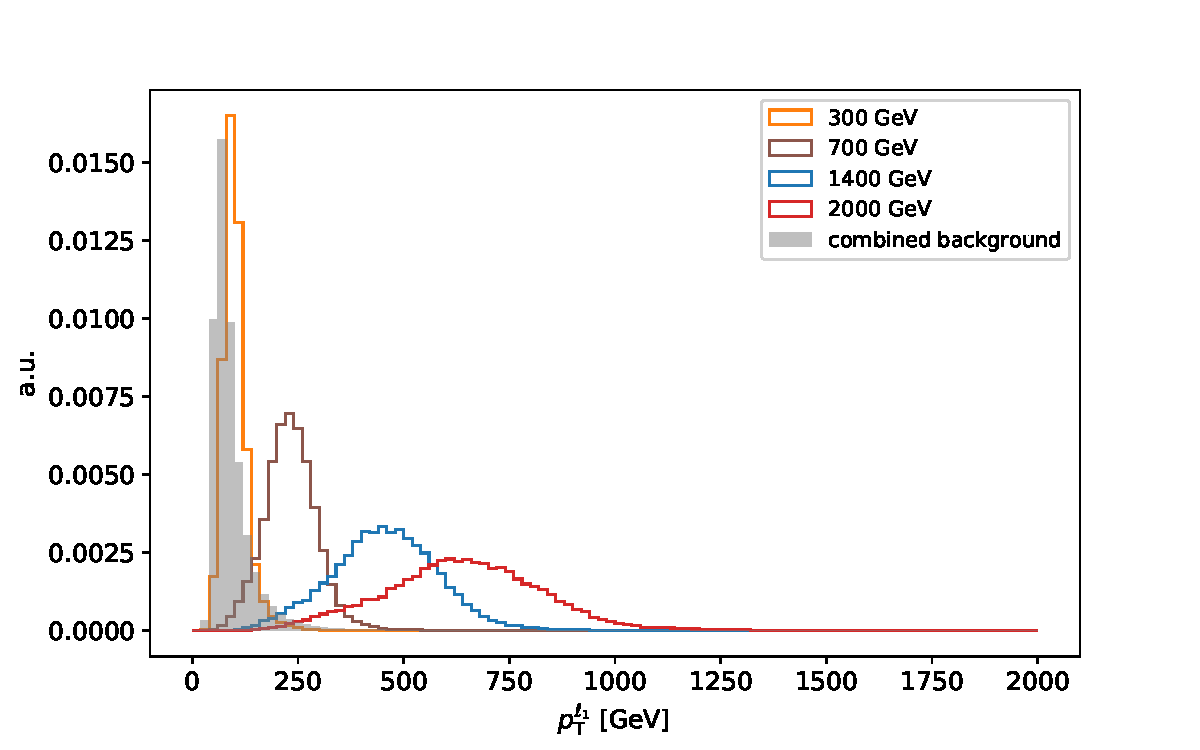
\includegraphics[width=0.24\textwidth]{figures/HMHZZ/selection/ggf_input/input_comparison_300_to_2000_15_score_lep_1_pt}}
%        \subfloat[]{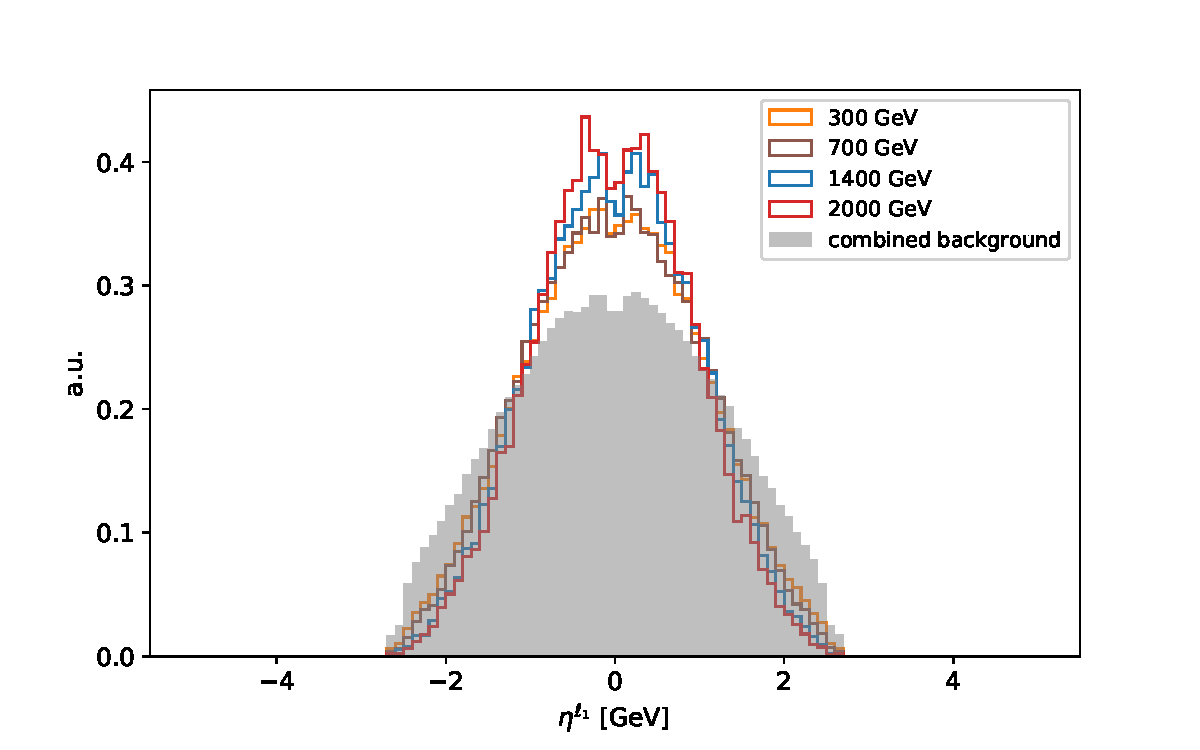
\includegraphics[width=0.24\textwidth]{figures/HMHZZ/selection/ggf_input/input_comparison_300_to_2000_16_score_lep_1_eta}}
%        \subfloat[]{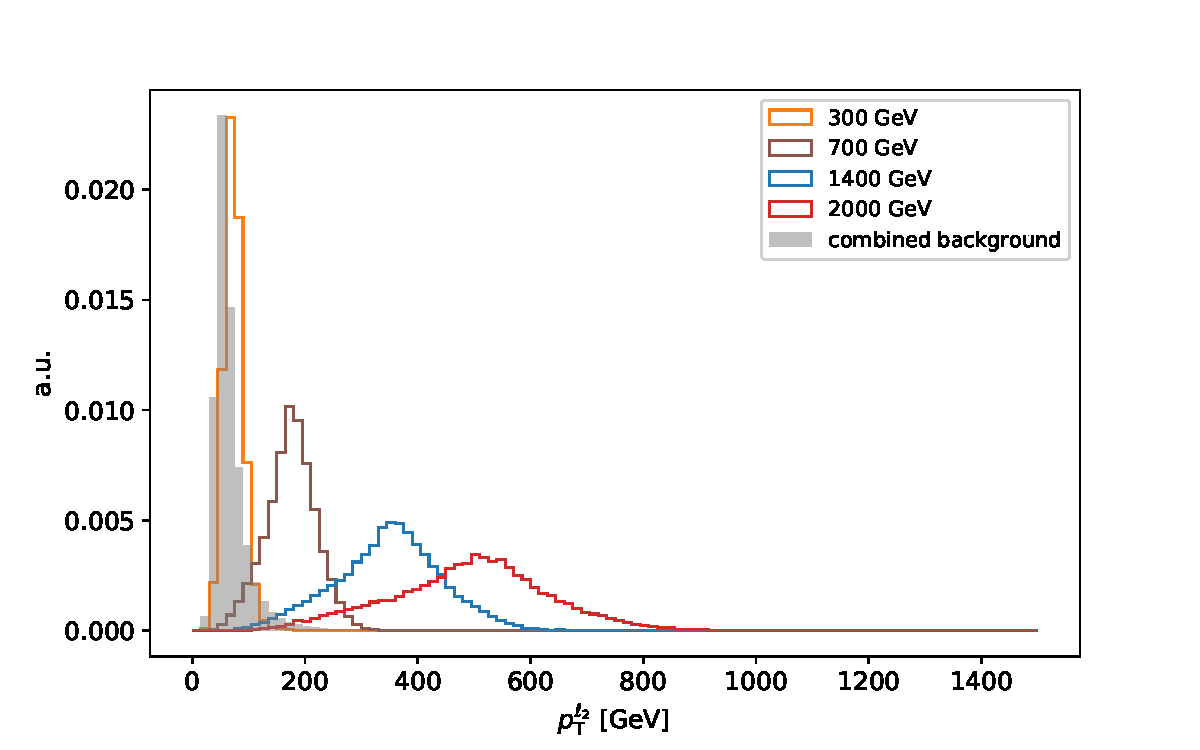
\includegraphics[width=0.24\textwidth]{figures/HMHZZ/selection/ggf_input/input_comparison_300_to_2000_17_score_lep_2_pt}}
%        \subfloat[]{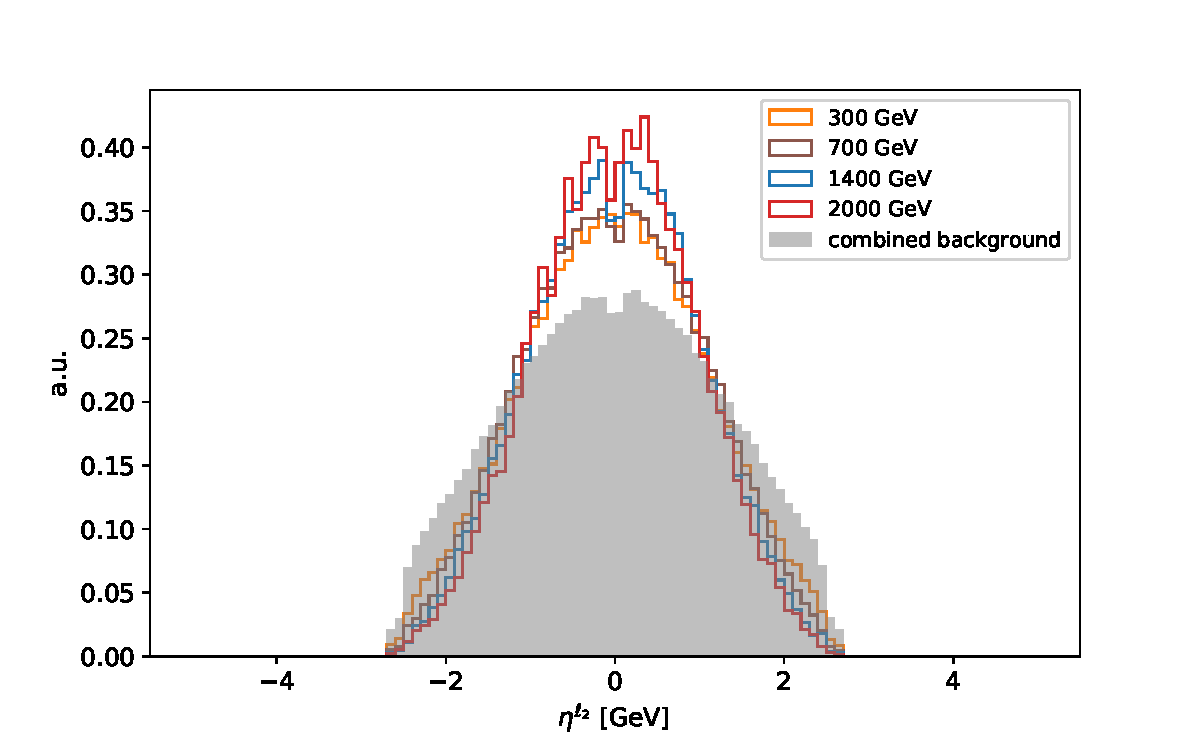
\includegraphics[width=0.24\textwidth]{figures/HMHZZ/selection/ggf_input/input_comparison_300_to_2000_18_score_lep_2_eta}}\\
%
%        \subfloat[]{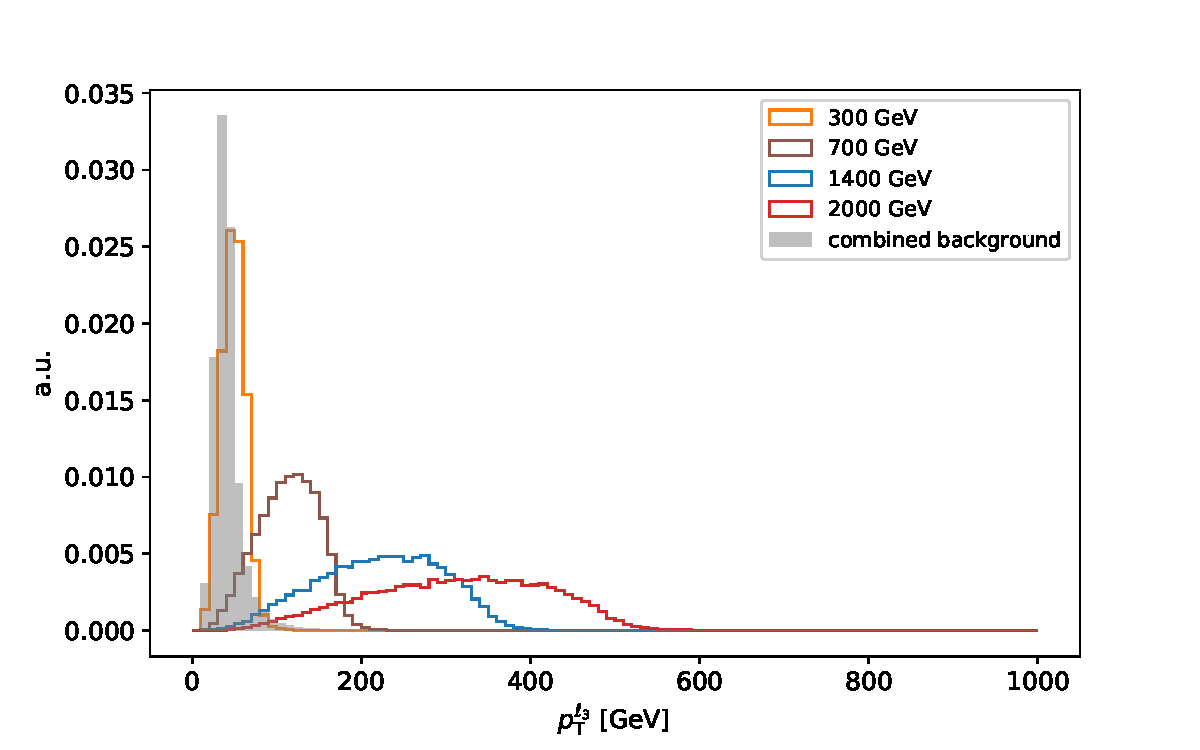
\includegraphics[width=0.24\textwidth]{figures/HMHZZ/selection/ggf_input/input_comparison_300_to_2000_19_score_lep_3_pt}}
%        \subfloat[]{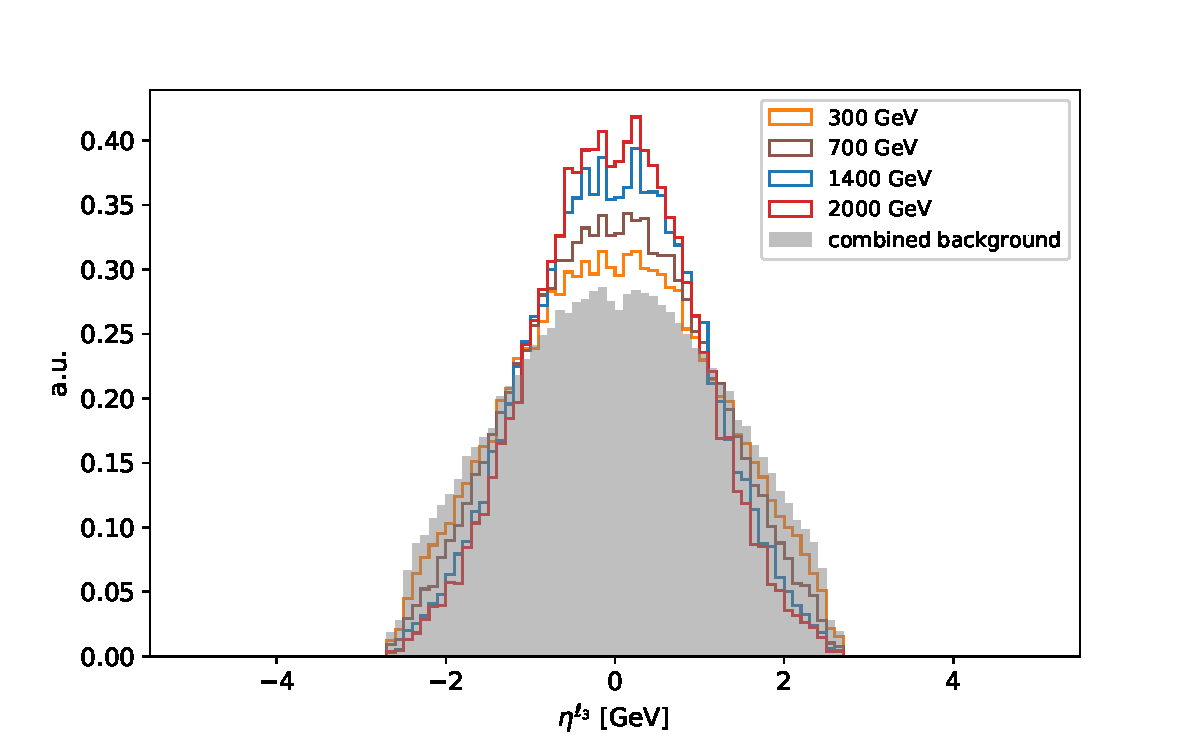
\includegraphics[width=0.24\textwidth]{figures/HMHZZ/selection/ggf_input/input_comparison_300_to_2000_20_score_lep_3_eta}}
%        \subfloat[]{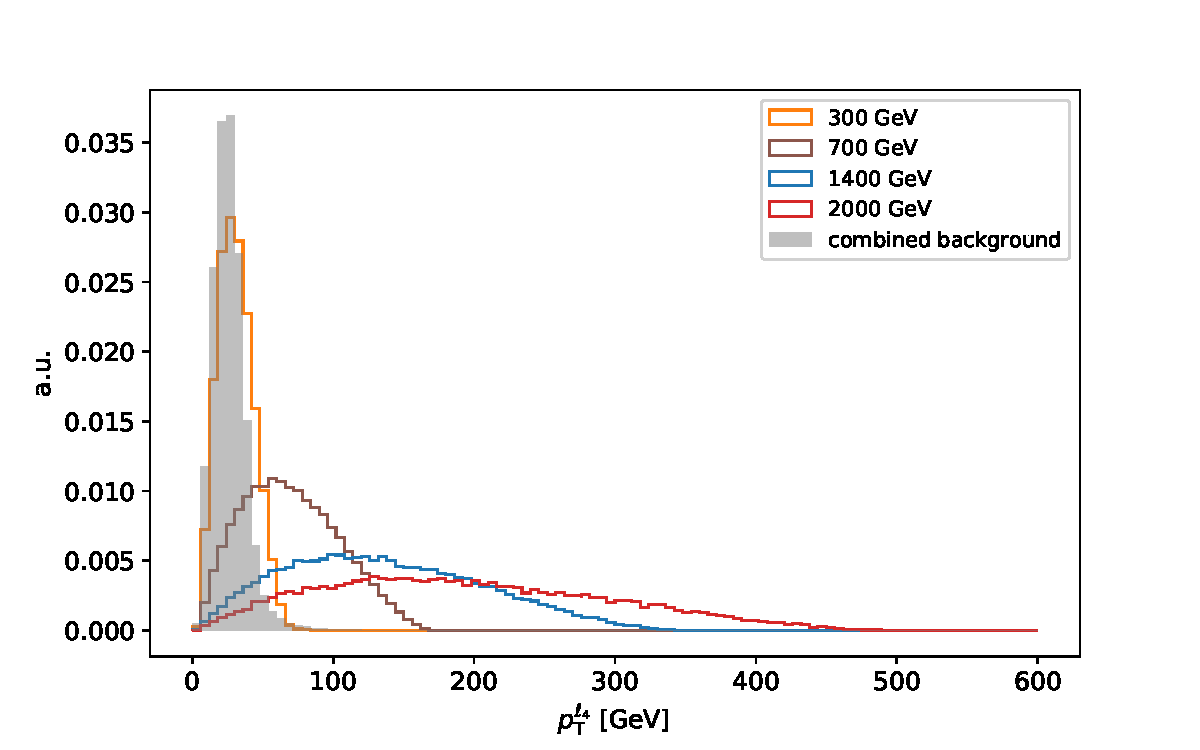
\includegraphics[width=0.24\textwidth]{figures/HMHZZ/selection/ggf_input/input_comparison_300_to_2000_21_score_lep_4_pt}}
%        \subfloat[]{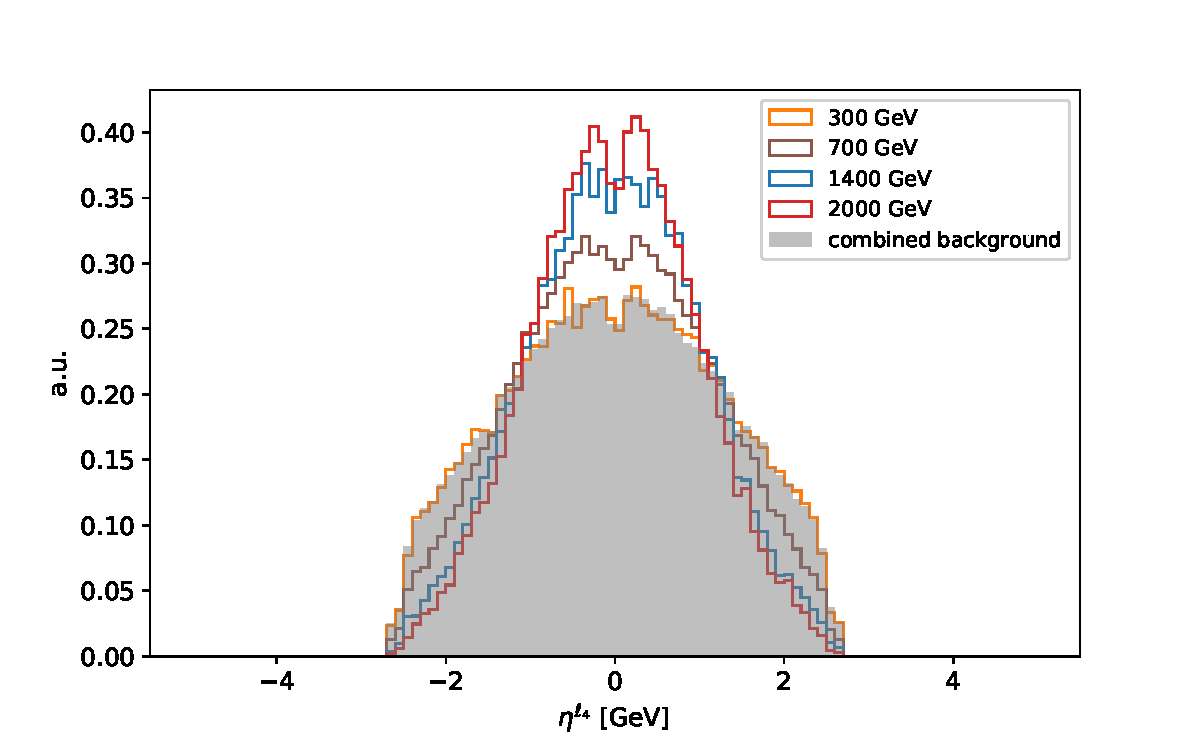
\includegraphics[width=0.24\textwidth]{figures/HMHZZ/selection/ggf_input/input_comparison_300_to_2000_22_score_lep_4_eta}}\\
%
%        \caption{Distributions of input features as listed in table~\ref{tab:dnn_features_ggf} for the ggF network of signals at mass points of 300, 700, 1400, 2000~\gev (coloured) and the background (grey). Events with any jet multiplicity are shown, as this model is evaluated in both $N_\mathrm{jets}\geq2$ and $N_\mathrm{jets}<2$.}
%        \label{fig:dnn_ggf_distribution}
%\end{figure}

\textbf{Evaluation of models} 

Figure~\ref{fig:dnn_output_score} shows the output of ``ggF-classifier'' and ``VBF-classifier'' for data, SM backgrounds and an example signal at 600~\gev.
The ggF and VBF signals cross section are set to be 100 times of their observed upper limit described in section~\ref{sec:hmhzz_spin0nwa} for ggF output
and 30 times of the observed upper limit for VBF output for best visibility.

\begin{figure}[htbp]
        \subfloat[]{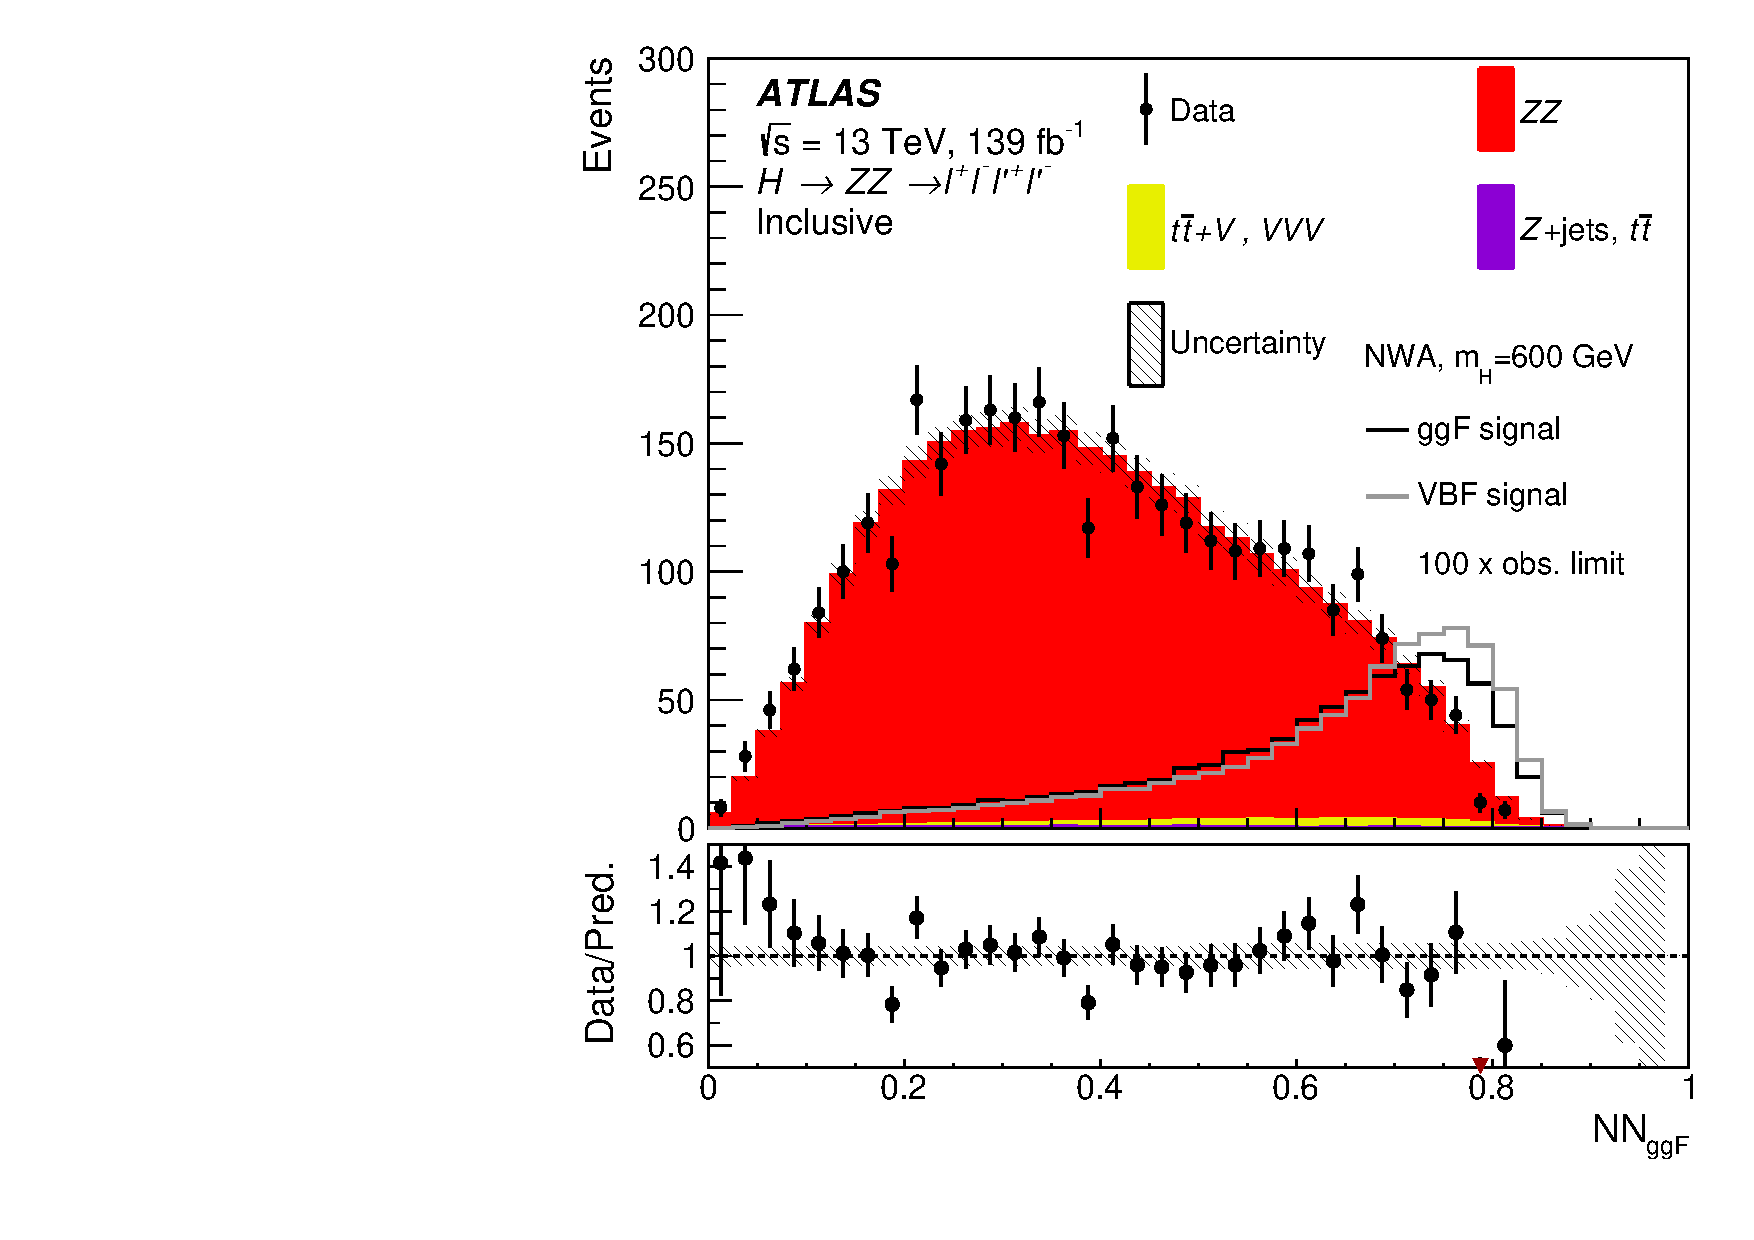
\includegraphics[width=0.48\textwidth]{figures/HMHZZ/results/4l_DNN_scores_ggF_incl.pdf}}
        \subfloat[]{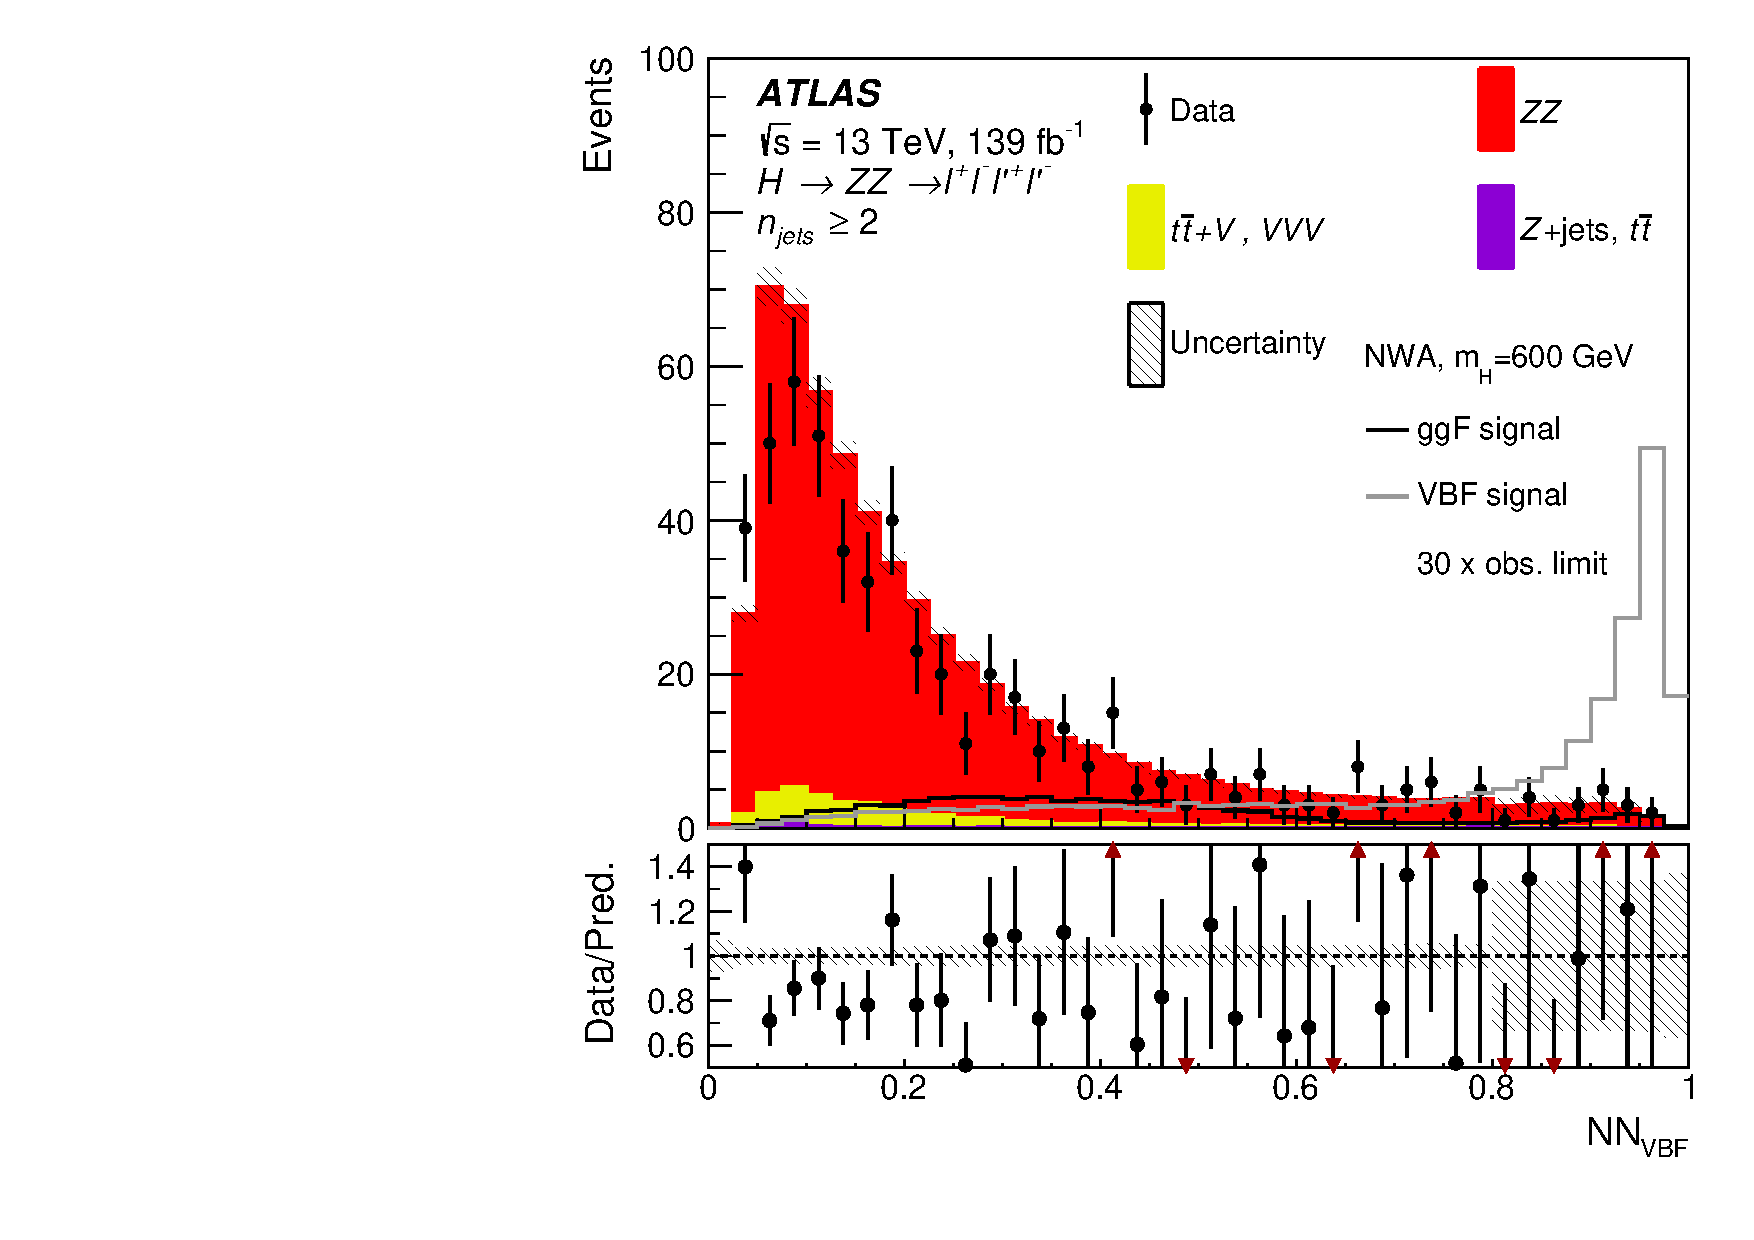
\includegraphics[width=0.48\textwidth]{figures/HMHZZ/results/4l_DNN_scores_VBF_incl.pdf}}
        \centering
        \caption{The output score of ``ggF-classifier'' (a) and  ``VBF-classifer'' (b) with the events passing the common event selections  
        for the data, the SM backgrounds and an example of a NWA signal with a mass of $600~\gev{}$.
        For the ``VBF-classifier'', an additional requirement of at least two jets in the event is applied.
        The signals cross section are set to 100 times of the observed limit for the ``ggF-classifier'' 
        and 30 times of the observed limit for the ``VBF~-classifer''.
        The $ZZ$ backgrounds are scaled by the normalisation factors shown in Table~\ref{tab:muZZ_bonly_dnn}.
        The lower panels show the ratio of data to prediction.
        Statistical and experimental systematic uncertainties are included.}
        \label{fig:dnn_output_score}
\end{figure}

Then the optimal cut at output score from each classifier is chosen based on an overall good performance of classifier to have a large significance improvement while retaining a high signal efficiency.
Figure~\ref{fig:dnn_significance} shows the significance improvements of MVA-based cuts when comparing with cut-based one at different VBF (left) and ggF (right) mass samples,
where the significance is calculated from an asymptotic approximation~\cite{2008NIMPA.595..480C}:
\begin{equation}
Z = \sqrt{2\left(n\ln \left[ \frac{nb+\sigma_b^2}{b^2+n\sigma_b^2}\right]
        - \frac{b^2}{\sigma_b^2}\ln\left[1+\frac{\sigma_b^2(n-b)}{b(b+\sigma_b^2)}\right]\right)}
\end{equation}
where n denotes to the sum of expected signal and background, b is the background, and $\sigma_b$ is the uncertainty of background.
Cut at 0.5 (0.8) for VBF (ggF) classifier is chosen as shown in solid lines.

\begin{figure}[htbp]
        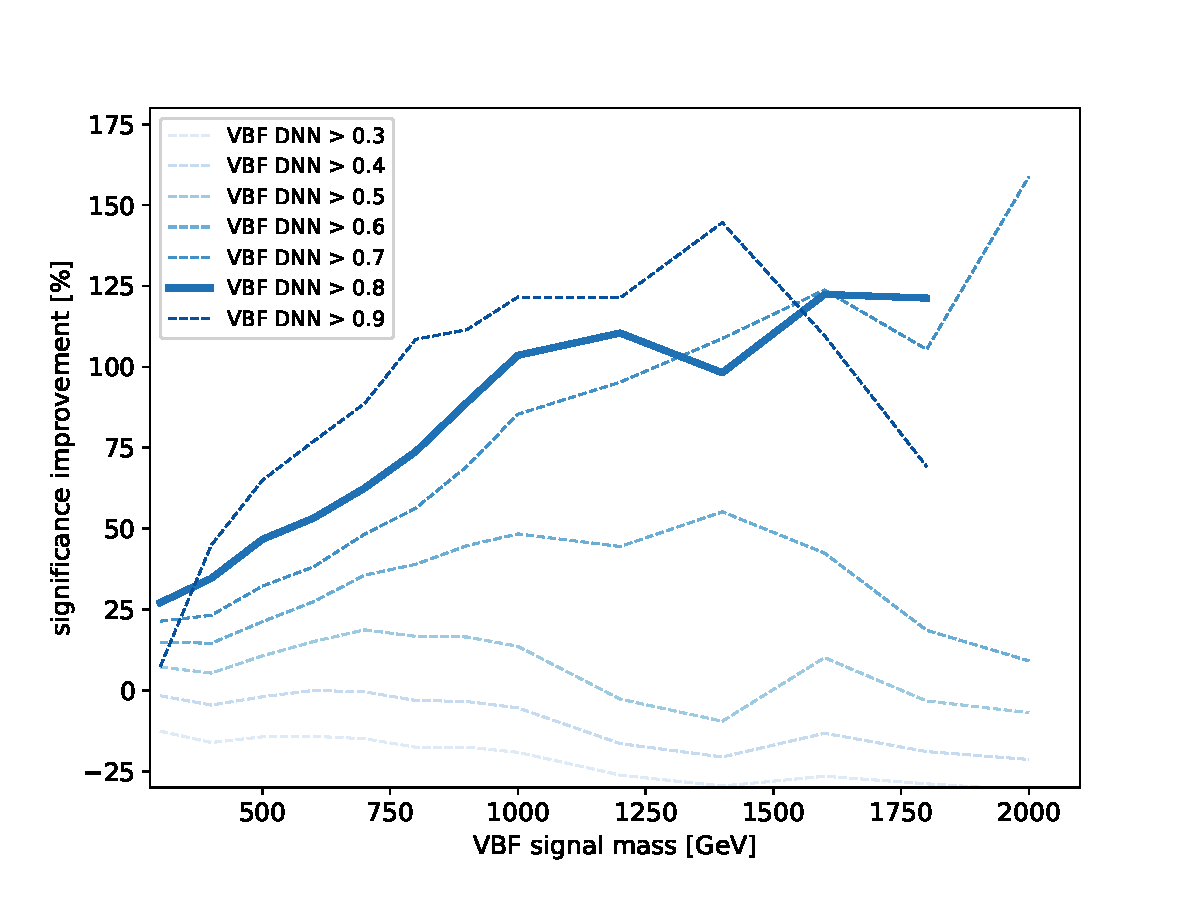
\includegraphics[width=0.48\textwidth]{figures/HMHZZ/selection/VBF_significance_improvement.pdf}
        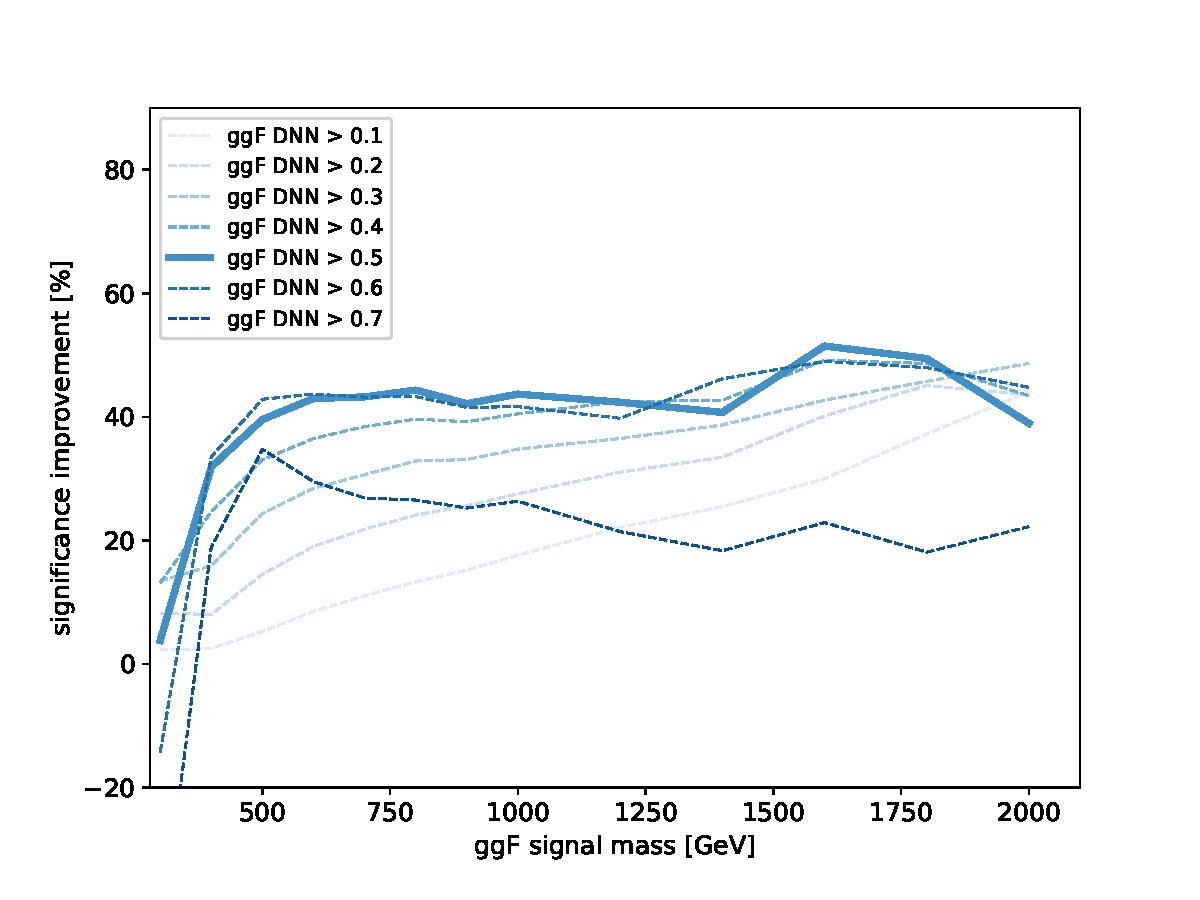
\includegraphics[width=0.48\textwidth]{figures/HMHZZ/selection/ggf_significance_improvement.pdf}
        \centering
        \caption{Significance improvements of the MVA-based over the cut-based categorization of the VBF (ggF) category for VBF (ggF) signal samples from 300 to 2000~\gev~ for seven different cuts on the VBF (ggF) output score. 
	The optimal cut of 0.8 (0.5) for VBF (ggF) score is chosen as the solid line, while other alternative cuts are plotted with dashed lines. 
	For VBF category, results at 2000~\gev~ for cuts of 0.8 and 0.9 are missing due to a lack of background events passing this tight selection.}
        \label{fig:dnn_significance}
\end{figure}

Then the events passing VBF classifier are categorized into VBF-MVA-enriched category.
Otherwise, the events failing VBF classifier but passing ggF classifier are categorized into ggF-MVA-high category, which is further split into 3 channels based on their lepton flavor.
All remaining events are sorted into one additional ggF-MVA-low category.
Thus there are five categories defined in MVA-based categorization.
In summary, cuts applied in categorization are defined as follow, and these different phase spaces are also illustrated in figure~\ref{fig:hmhzz_dnncate}.

\begin{itemize}
	\item VBF-MVA-enriched category: Events have at least two selected jets ($\Njets \geq 2$), and with \DNNVBF > 0.8;
	\item ggF-MVA-high categories: $(\Njets \geq 2 \:\&\&\: \DNNVBF \leq 0.8 \:\&\&\: \DNNggF > 0.5) \:||\: (\Njets < 2 \:\&\&\: \DNNggF > 0.5)$; 
	\item ggF-MVA-low category: All remaining events that fail VBF and ggF cuts mentioned above.
\end{itemize}

\begin{figure}[h]
\centering
\subfloat[]{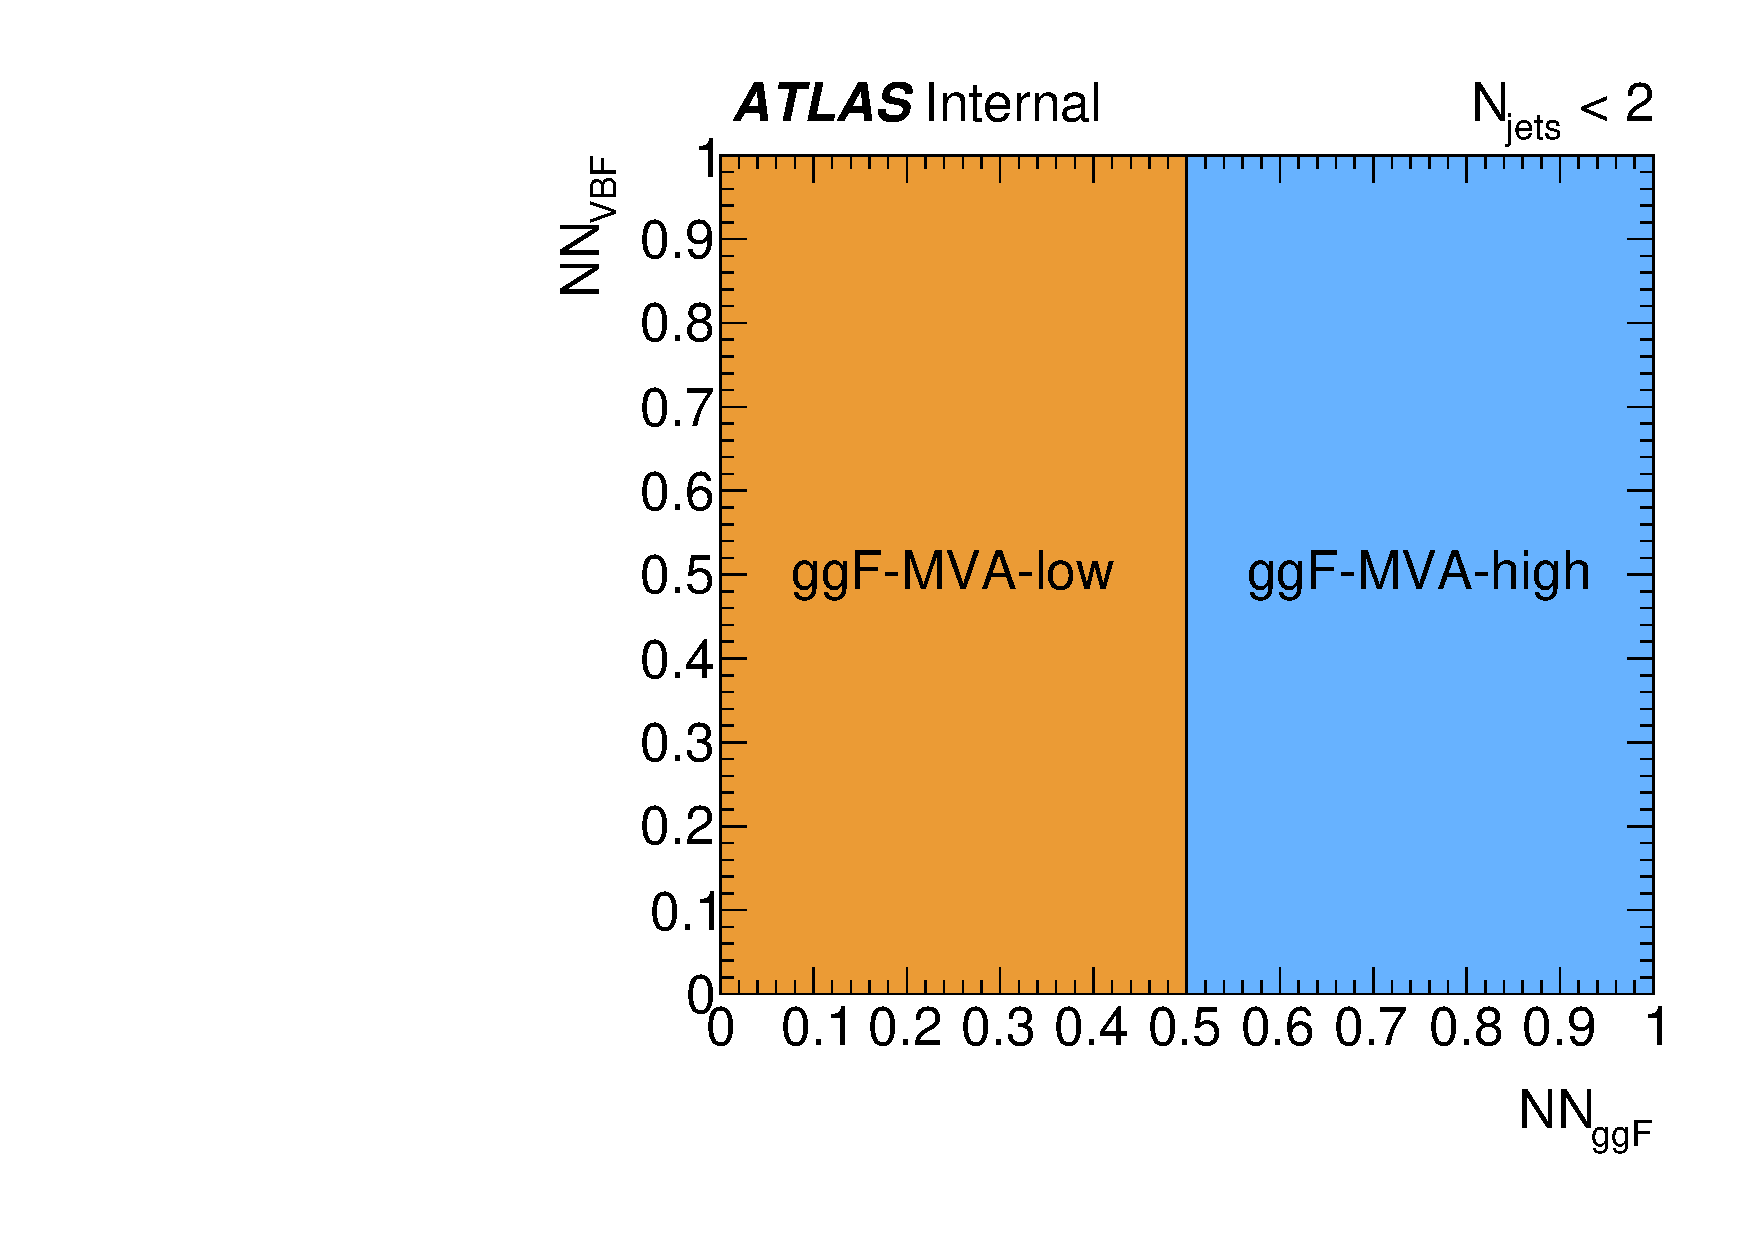
\includegraphics[width=0.43\textwidth]{figures/HMHZZ/selection/classifier_diagram_c1_njets_lt2.pdf}}
\subfloat[]{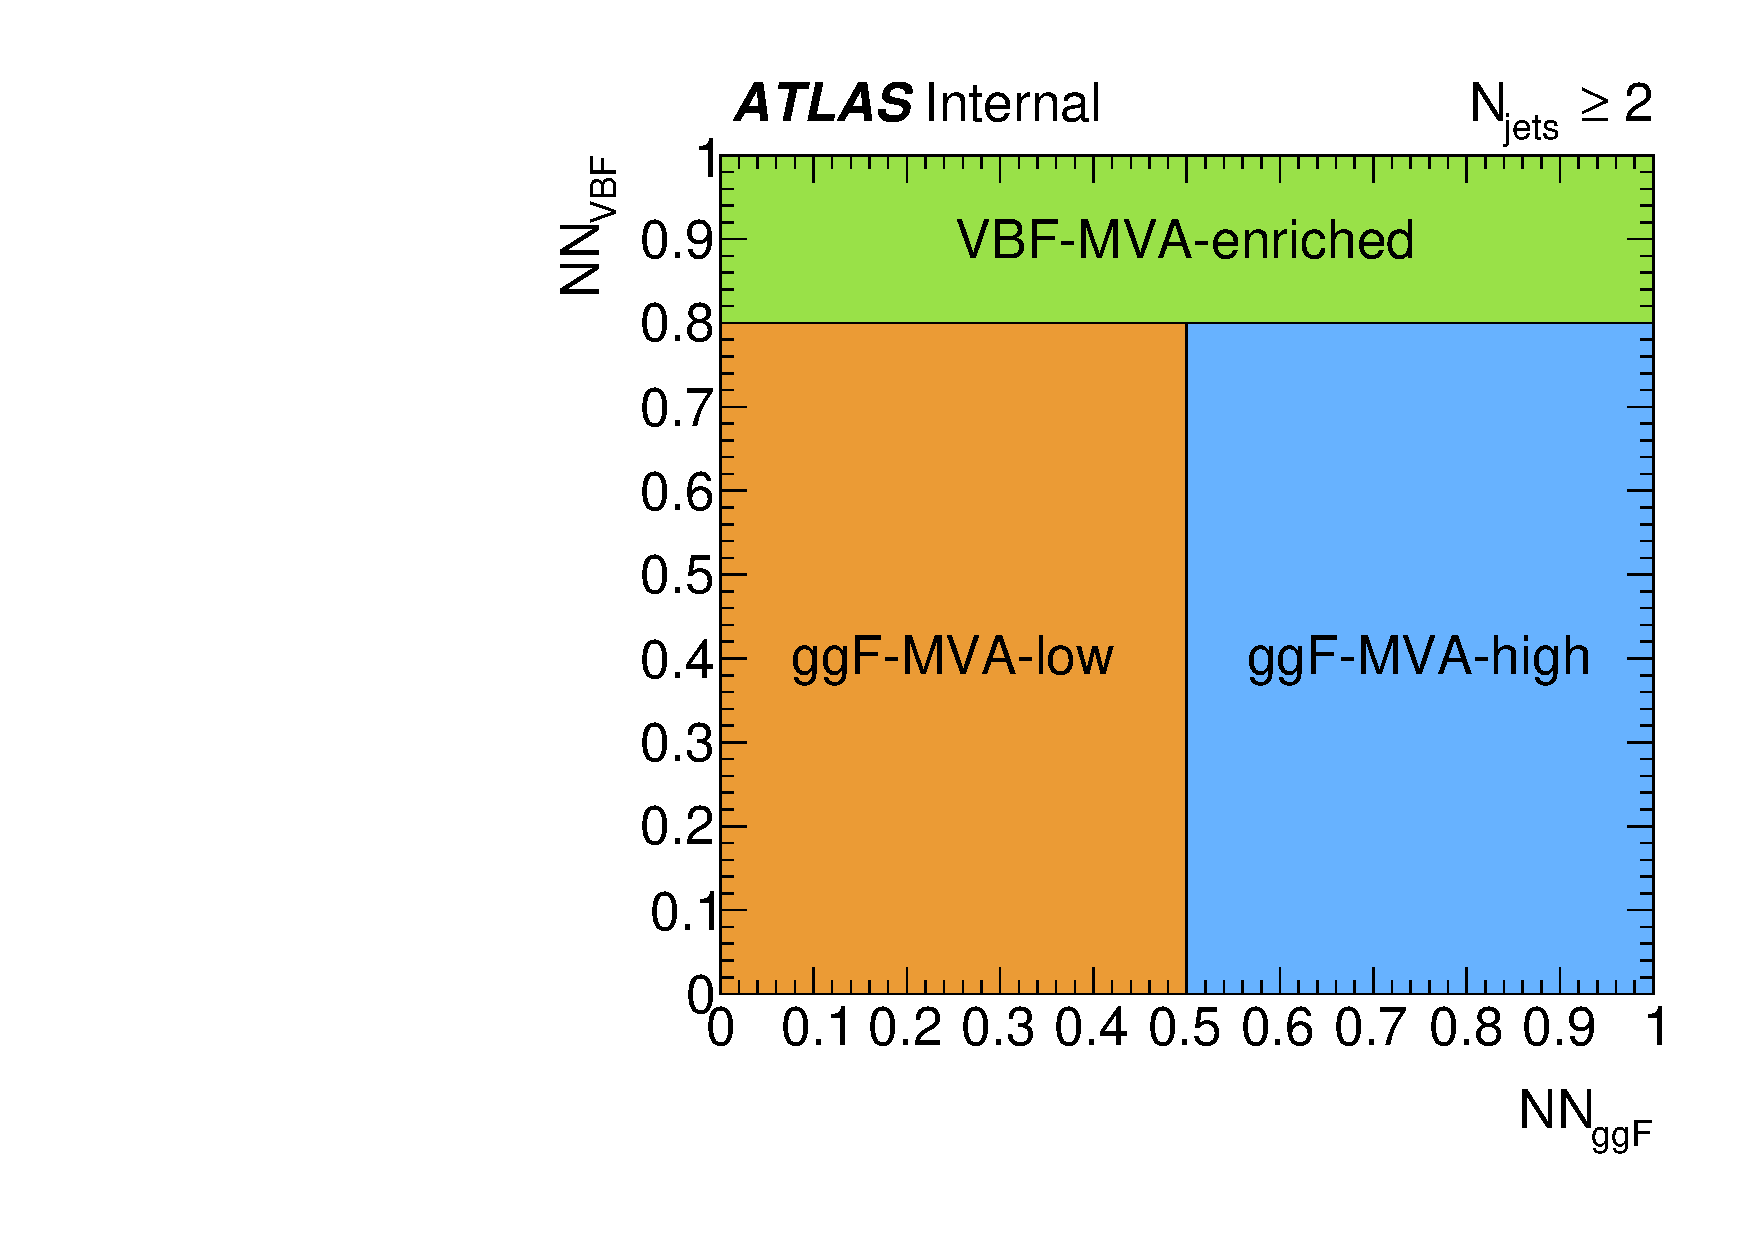
\includegraphics[width=0.43\textwidth]{figures/HMHZZ/selection/classifier_diagram_c1_njets_gt2.pdf}}\\
\caption{Illustration of the MVA-based VBF and ggF event classification for events with (a) $\Njets < 2$ and (b) $\Njets \geq 2$.}
\label{fig:hmhzz_dnncate}
\end{figure}

\subsection{Signal acceptance} 
\label{sec:hmhzz_signal_acc}
The signal acceptance is defined as the ratio of events passing all analysis selection in each category to the total number of simulated events in whole phase space.
In denominator, the events with $\tau$ final states are not taken into account.
And the contribution of $\tau$-lepton decay to electrons and muons final states is found to be negligible.

Figure~\ref{fig:hmhzz_acc_dnn} and ~\ref{fig:hmhzz_acc_cut} show the acceptance of NWA signals in DNN- and Cut- based categorization, estimated by merging the three signal MC campaigns, mc16a, mc16d and mc16e.
A 3-rd order polynomial fit is applied for each category.

\begin{figure}[h]
\centering
\subfloat[]{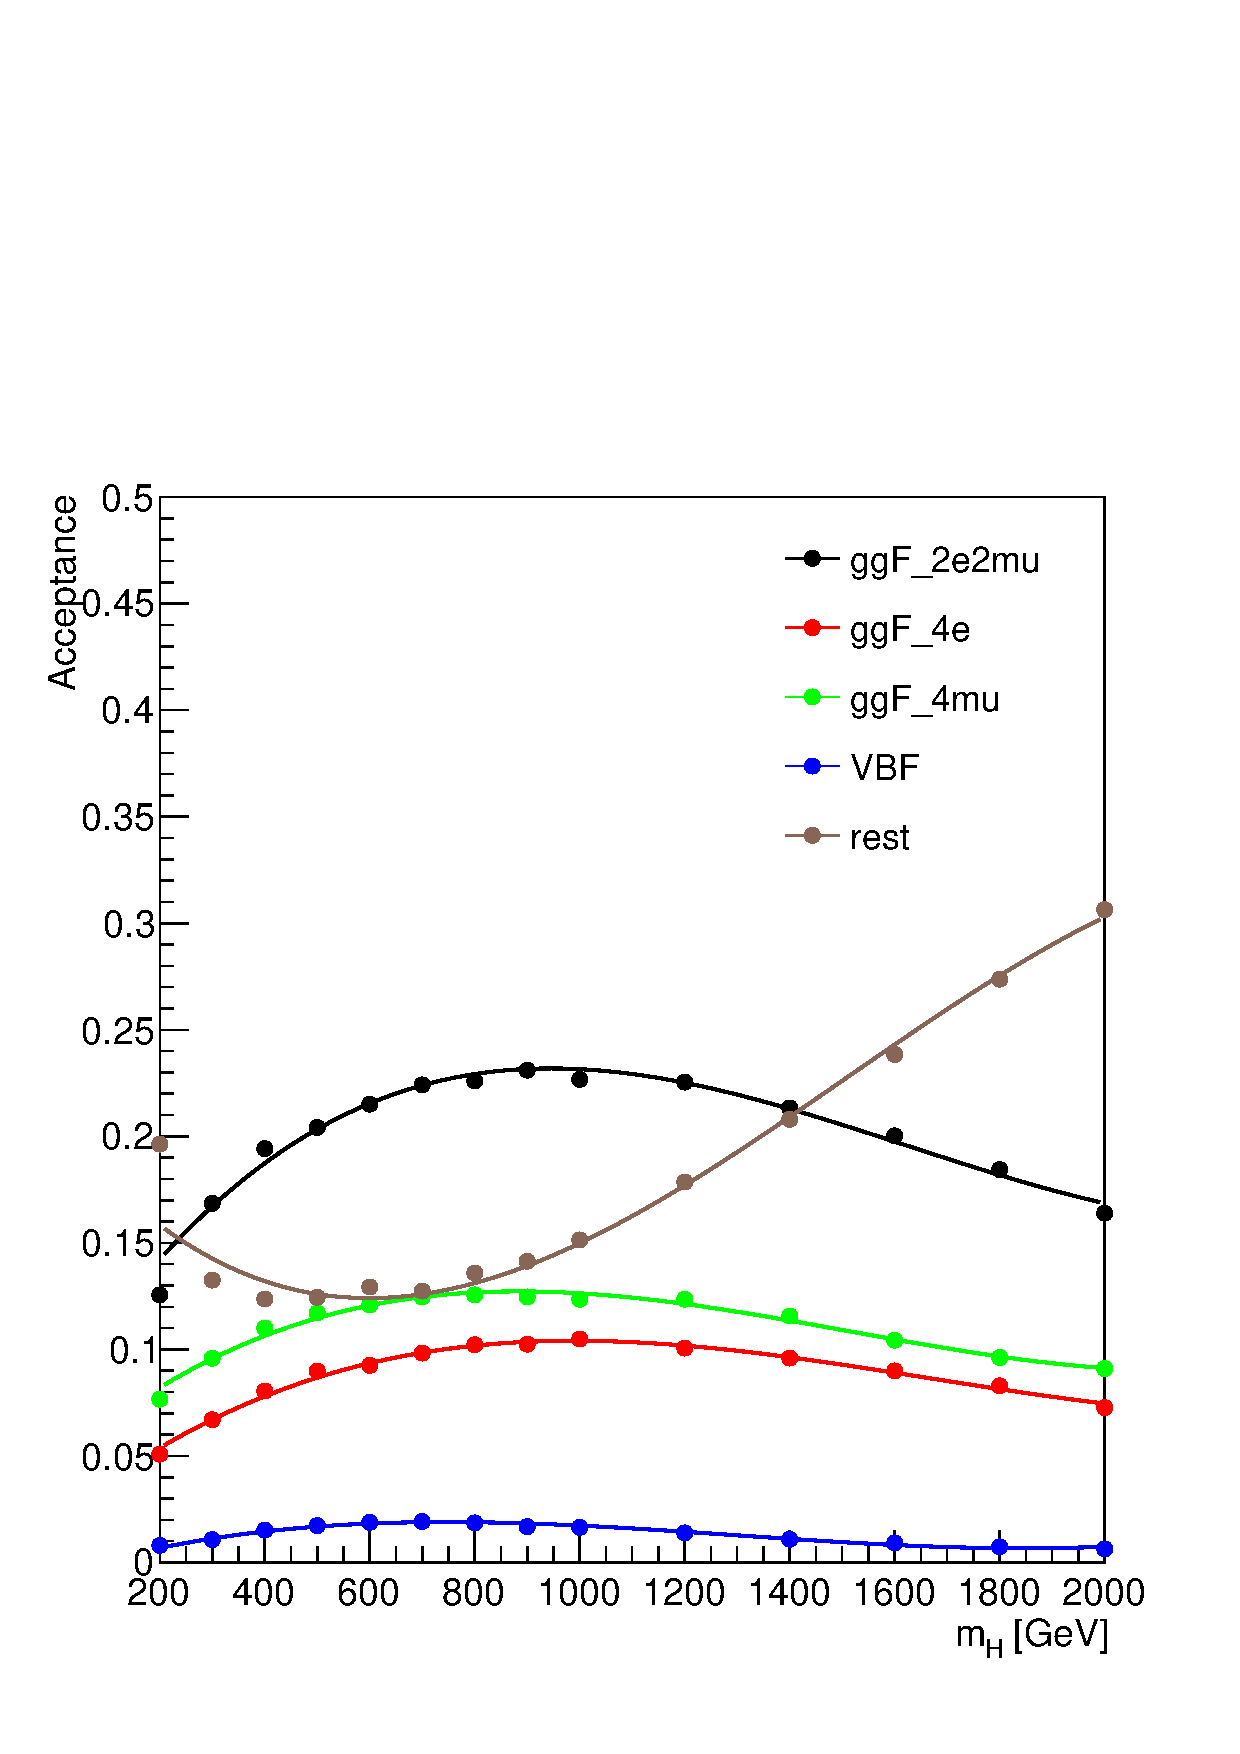
\includegraphics[width=0.43\textwidth]{figures/HMHZZ/selection/acc_dnn_ggF.pdf}}
\subfloat[]{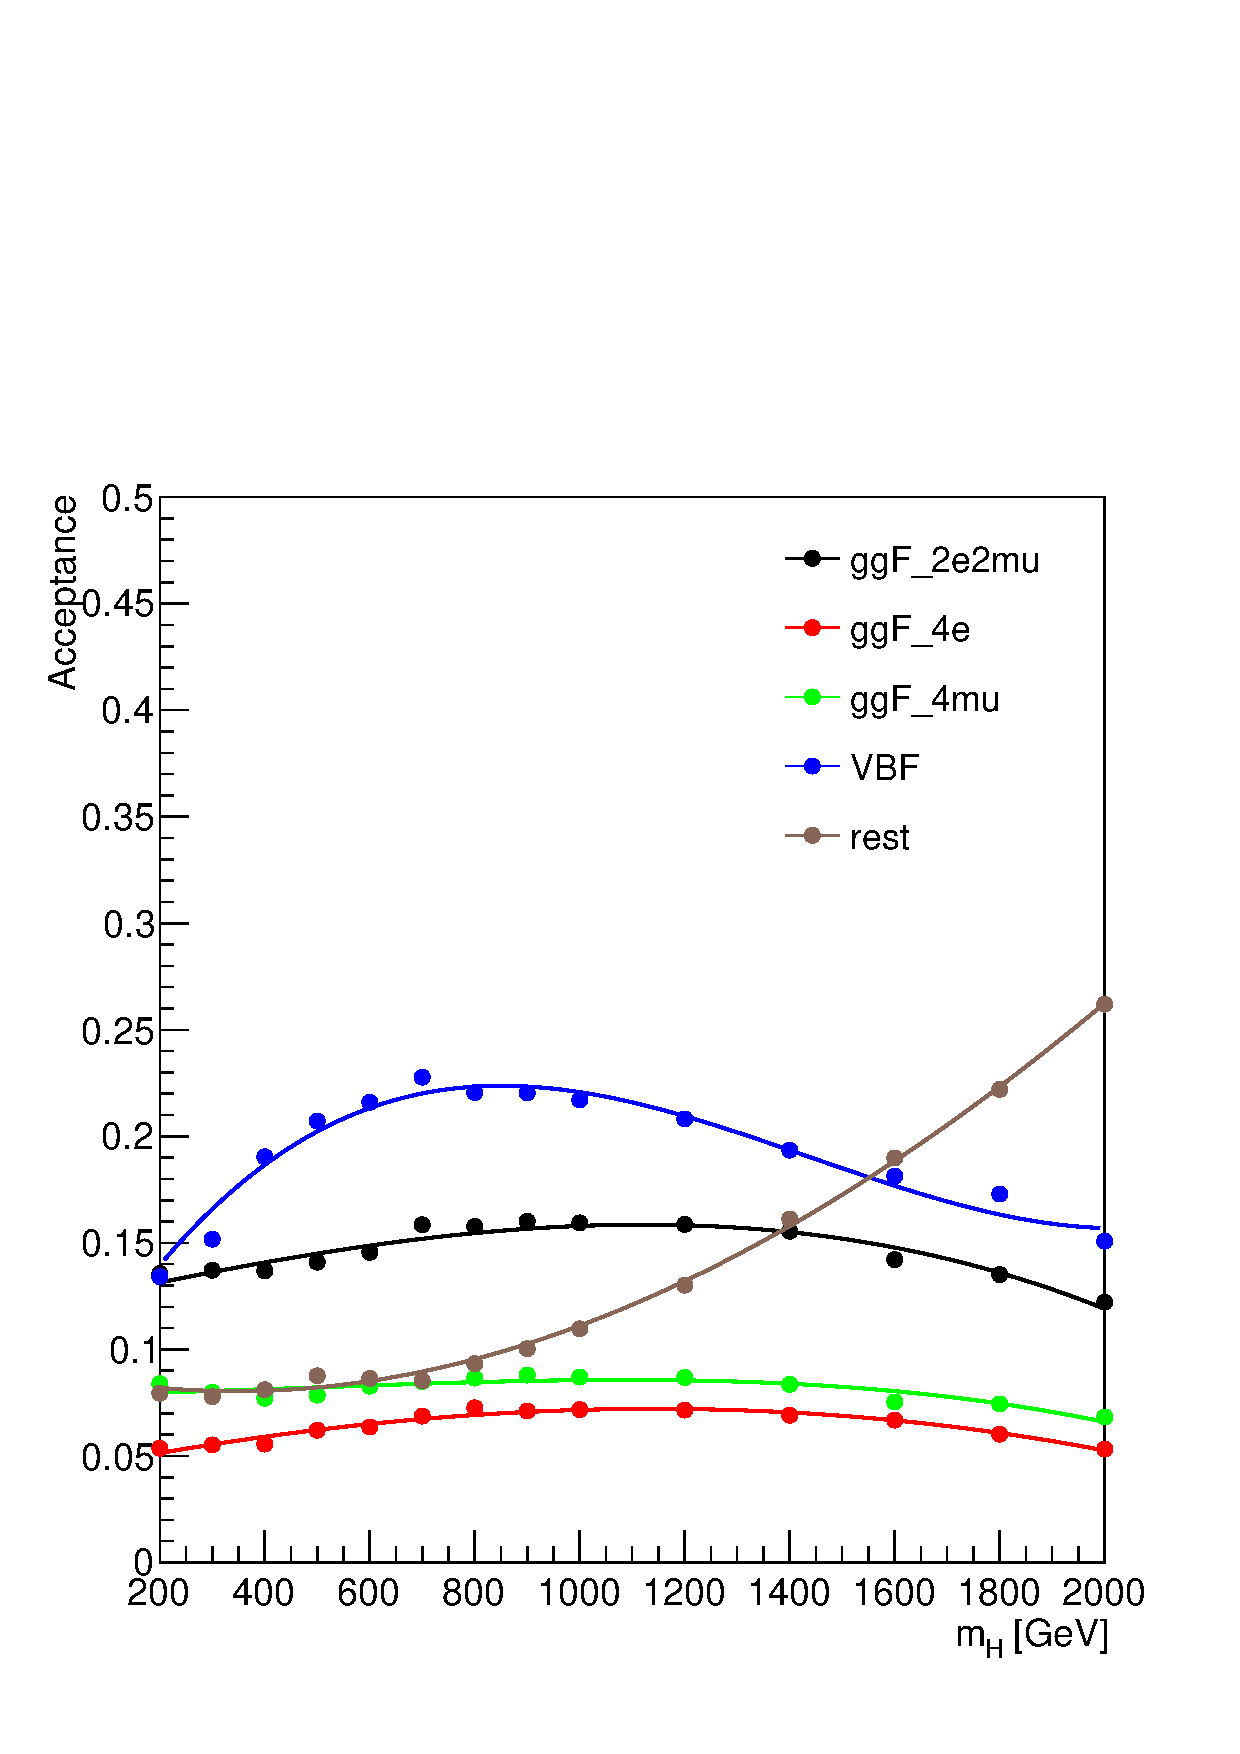
\includegraphics[width=0.43\textwidth]{figures/HMHZZ/selection/acc_dnn_VBF.pdf}}\\
\caption{NWA acceptance as a function of $m_{H}$ for the MVA-based categorization for the samples of
(a) ggF production;
(b) VBF production. 
}
\label{fig:hmhzz_acc_dnn}
\end{figure}

\begin{figure}[h]
\centering
\subfloat[]{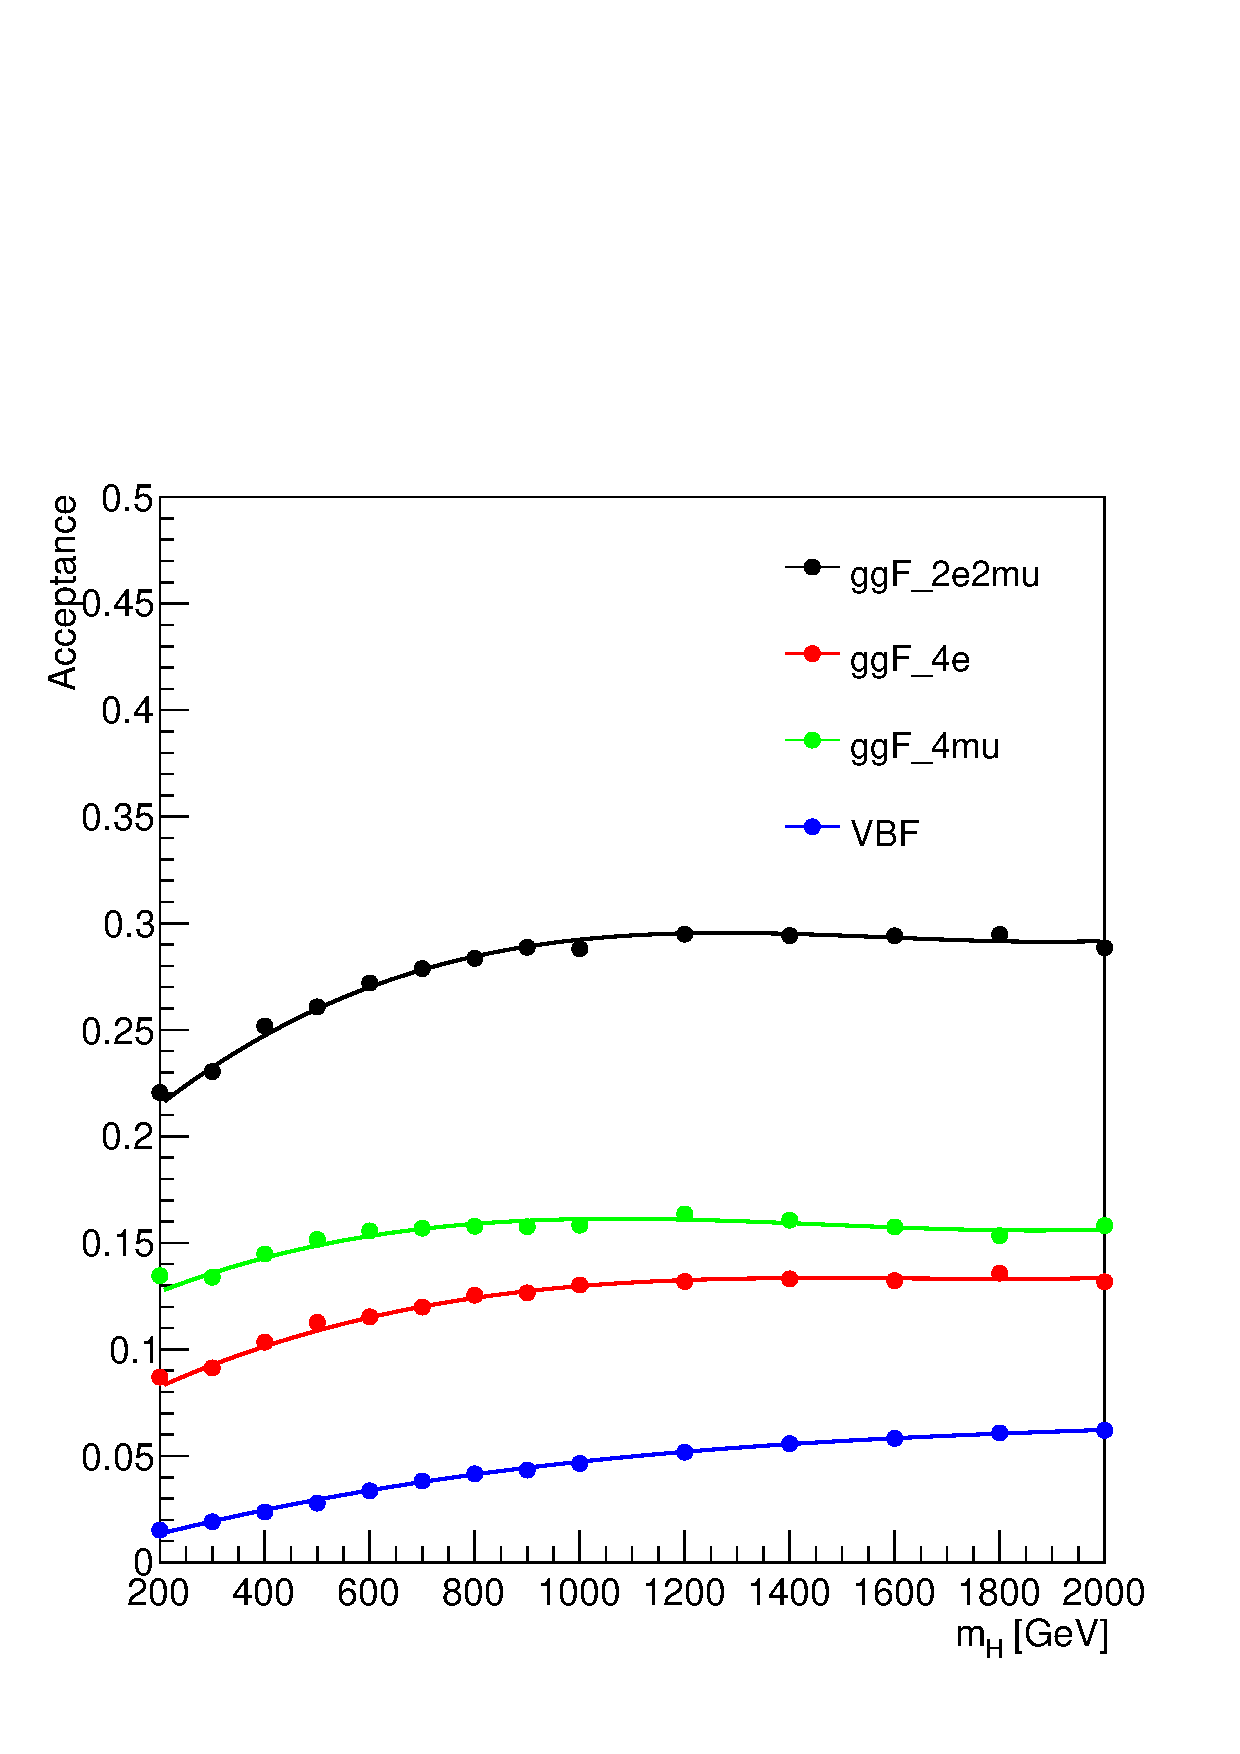
\includegraphics[width=0.43\textwidth]{figures/HMHZZ/selection/acc_cut_ggF.pdf}}
\subfloat[]{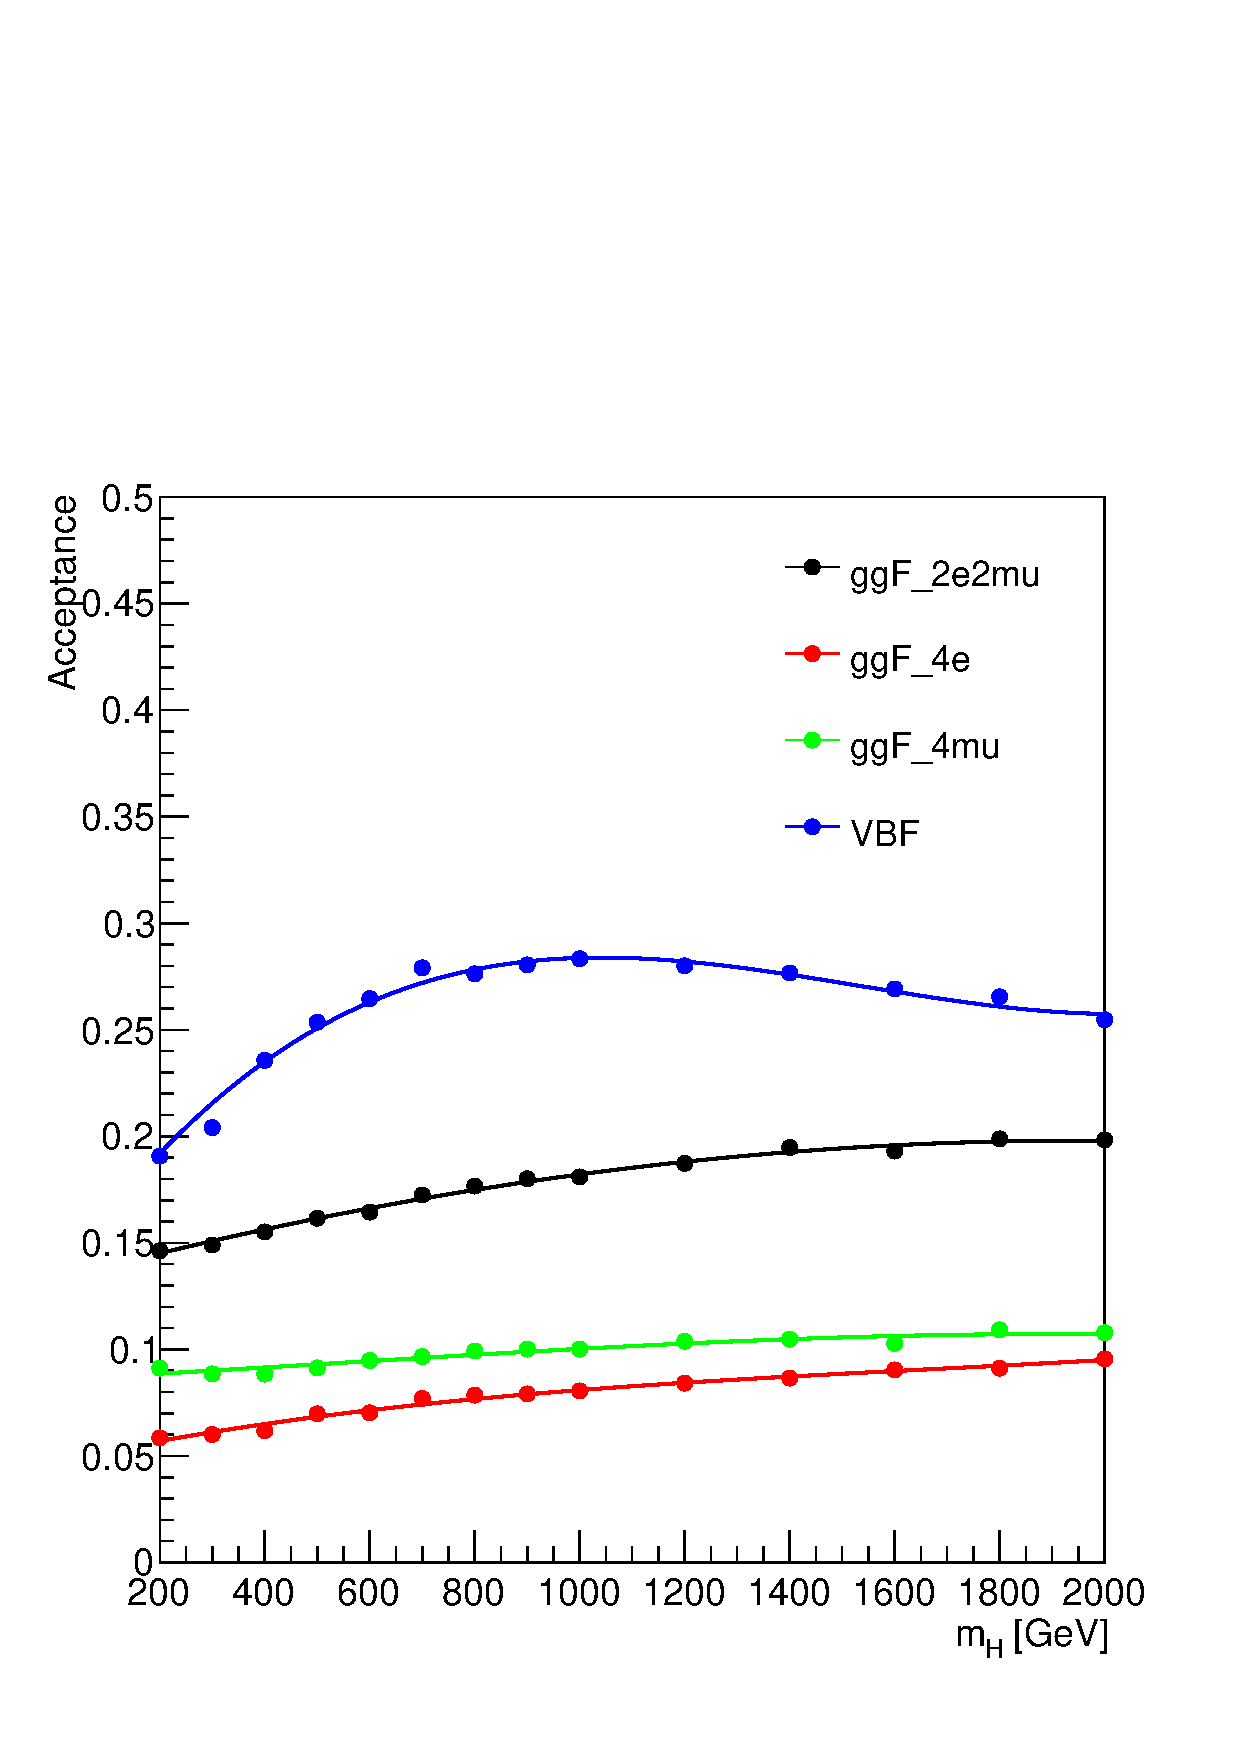
\includegraphics[width=0.43\textwidth]{figures/HMHZZ/selection/acc_cut_VBF.pdf}}\\
\caption{NWA acceptance as a function of $m_{H}$ for the Cut-based categorization for the samples of
(a) ggF production mode;
(b) VBF production mode. }
\label{fig:hmhzz_acc_cut}
\end{figure}

